\section{Experimental Results}
\label{sec:pmc-results}

This section presents comprehensive results for predicting memory consumption in seismic workloads based on their \ac{3D} input shapes.
We organize the findings into four main categories:
(i) memory and execution-time profiling,
(ii) model performance overview,
(iii) feature selection experiments,
and (iv) data reduction studies.
Each category reveals different facets of how shape parameters affect resource requirements, model behavior, and prediction robustness.
All code, scripts, and output files that underlie these analyses reside in the \texttt{experiment} directory of the project repository~\cite{delucca2025experiment2results}.

\subsection{Experiment Outputs Overview}
\label{subsec:pmc-results-experiment-outputs-overview}

This subsection briefly outlines the three seismic operators examined (Envelope, \ac{GST3D}, and the 3D Gaussian Filter), underscores the main experimental objectives, and describes the key \ac{CSV} files generated during the final stages of the pipeline.
These \ac{CSV} artifacts are the foundation for the analyses presented in the following subsections.

\vspace{1em}
\noindent
\textbf{Operators and Experimental Goals.}
We investigated three commonly used seismic processing operators:
\begin{itemize}
    \item \emph{Envelope}: Computes instantaneous amplitude along seismic traces. 
    \item \emph{\ac{GST3D}}: Highlights discontinuities or faults using structural tensors.
    \item \emph{3D Gaussian Filter}: Applies a smoothing operation across volumes to reduce high-frequency noise.
\end{itemize}
All three involve memory-intensive operations on potentially large \ac{3D} volumes.
Our primary goal was to build regression models that predict each operator’s peak memory usage as a function of shape parameters (\textit{inlines}, \textit{xlines}, and \textit{samples}), enabling more accurate \ac{HPC} job submissions.

\vspace{1em}
\noindent
\textbf{Data Artifacts.}
During the final stage of the pipeline, five main \ac{CSV} outputs were generated:
\begin{enumerate}
    \item \emph{profile\_history.csv}: Stores time-series \ac{RSS} measurements and timestamps for each operator run. This file is useful for \EBRPD{detecting}{analyzing} moment-to-moment memory fluctuations.
    \item \emph{profile\_summary.csv}: Summarizes peak memory usage, execution time, and statistical descriptors (means, standard deviations, minima, and maxima) per volume configuration.
    \item \emph{model\_metrics.csv}: Captures regression model performances (\ac{RMSE}, \ac{MAE}, $R^2$, and accuracy metrics), along with arrays of predictions and residuals.
    \item \emph{feature\_selection.csv}: Documents experiments that limit the predictor set to specific features or transformations to assess their importance in predicting memory usage.
    \item \emph{data\_reduction.csv}: Compares how models behave when trained on progressively smaller subsets of the full dataset, providing insight into data requirements for stable predictions.
\end{enumerate}

\vspace{1em}
\noindent
\textbf{Shape Configurations.}
The synthetic seismic volumes encompassed a broad range of \ac{3D} shapes, from $100 \times 100 \times 100$ up to sizes near the system’s memory limits.
By spanning both small and large volumes, we could characterize memory usage trends across diverse problem scales.
Each operator was run on each shape variant, yielding a comprehensive grid of memory and runtime measurements.

\vspace{1em}
\noindent
\textbf{Chapter Roadmap.}
\EB{Acho que fica melhor remover o título "Chapter Roadmap." deste parágrafo.}
Section~\ref{sec:pmc-results-memory-and-execution-time-profiling} explores the memory-usage trends and execution-time patterns for each operator.
Subsequent sections delve into model performance, assessing how various feature sets and data volumes influence predictive accuracy.
We conclude by comparing Envelope, \ac{GST3D}, and Gaussian Filter side by side, identifying operator-specific nuances that can inform more reliable \ac{HPC} scheduling.
\section{Memory and Execution-Time Profiling}
\label{sec:pmc-results-memory-and-execution-time-profiling}

In this section, we focus on raw memory and execution-time measurements before discussing any modeling approach.
By examining usage patterns, run durations, and dimension-specific behaviors, we contextualize the challenges of predicting peak memory consumption in an \ac{HPC} setting.

\subsection{Linear Trends and Variability}
\label{subsec:linear-trends-and-variability}

Figure~\ref{fig:peak_memory_facet} shows how average peak memory usage tends to scale linearly with the overall volume (\(\text{inlines} \times \text{xlines} \times \text{samples}\)). 
\EB{Para refletir: Daniel, este gráfico por si só já mostra que existe uma relação quase linear entre a feature volume e o consumo de memória destes kernels. Fiquei na dúvida se faz sentido ter toda uma discussão sobre a relação entre as outras features e o consumo de memória depois de já concluir que há uma relação simples (linear) entre a feature volume e consumo de memória.}
The Envelope, \ac{GST3D}, and Gaussian Filter operators each display a relatively direct proportionality between volume and memory demand.
Interestingly, larger volumes produce consistently higher yet less variable memory consumption, whereas smaller volumes display higher \ac{CV}\EBRM{(coefficient of variation)}.

A possible explanation for this disparity is that smaller volumes involve shorter-run processes in which overheads (e.g., Python interpreter initialization, I/O buffering) can appear more prominently, thus creating variability.
As volumes grow, these overheads become negligible compared to the large data arrays and associated computations.
Consequently, memory usage “smooths out” and increasingly reflects the operator’s intrinsic workload characteristics.

\begin{figure*}[htbp]
    \centering
    \begin{subfigure}[t]{0.49\textwidth}
        \centering
        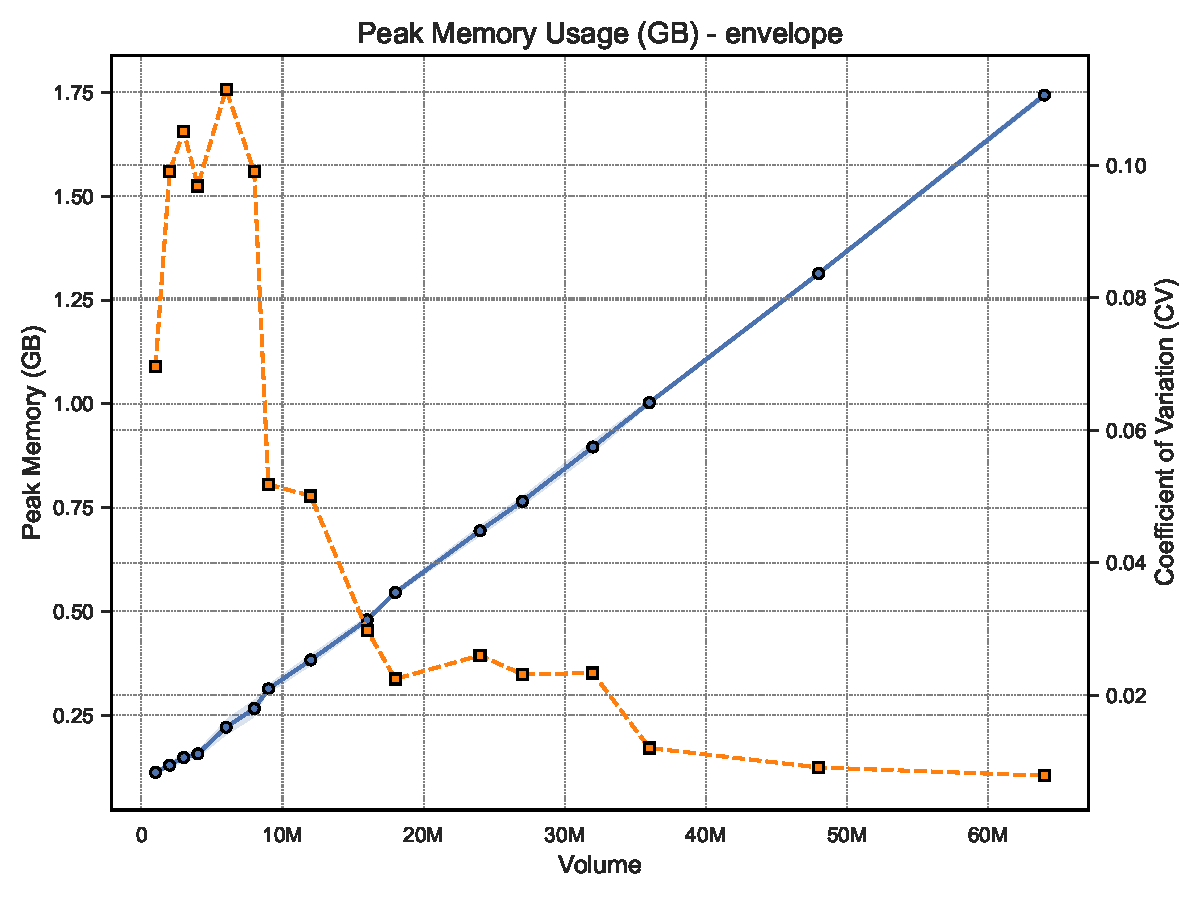
\includegraphics[width=\textwidth]{assets/images/05/peak_memory_by_volume_envelope}
        \caption{Envelope: Smaller volumes exhibit higher variability, while larger volumes show a consistent linear growth trend.}
    \end{subfigure}
    \hfill
    \begin{subfigure}[t]{0.49\textwidth}
        \centering
        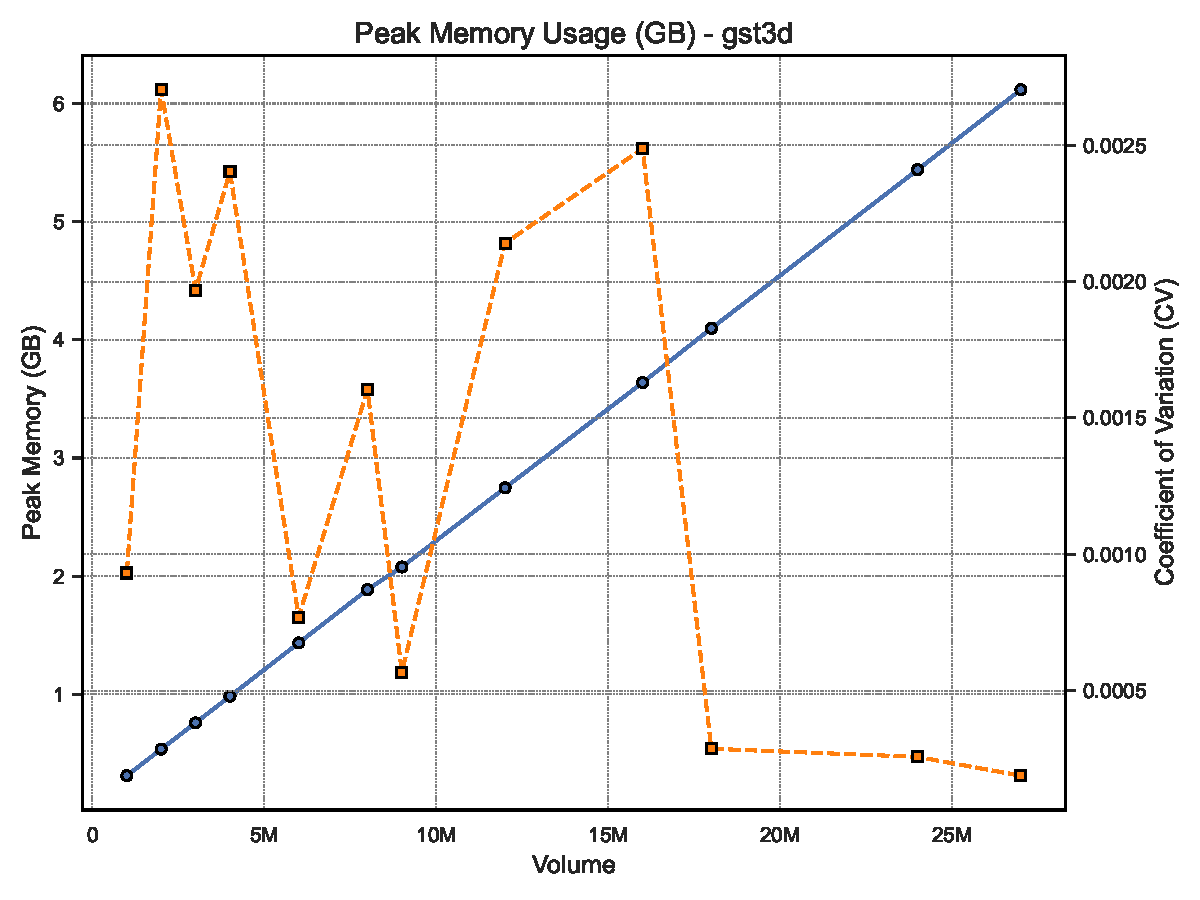
\includegraphics[width=\textwidth]{assets/images/05/peak_memory_by_volume_gst3d}
        \caption{\ac{GST3D}: This operator has a steeper slope compared to Envelope, reflecting more elaborate data structures.}
    \end{subfigure}
    \hfill
    \begin{subfigure}[t]{0.49\textwidth}
        \centering
        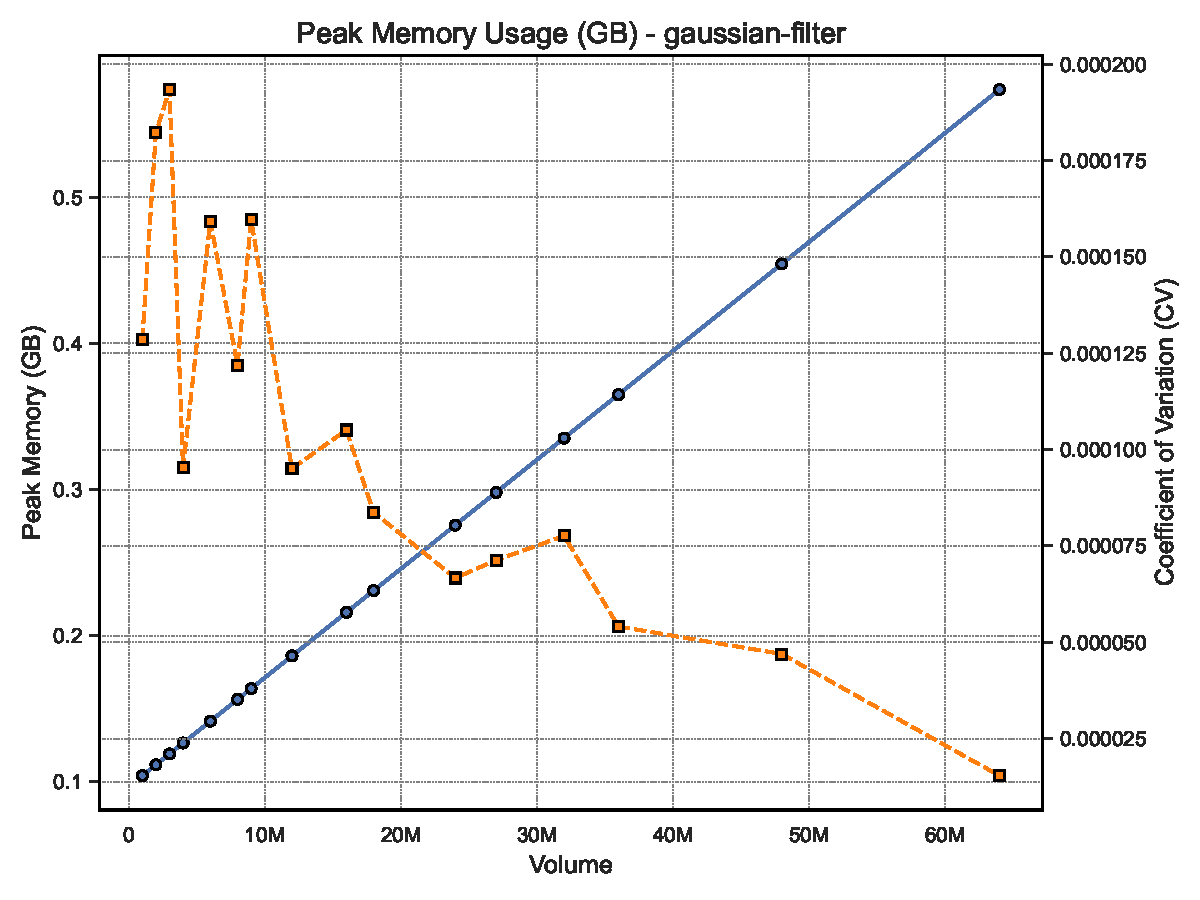
\includegraphics[width=\textwidth]{assets/images/05/peak_memory_by_volume_gaussian-filter}
        \caption{Gaussian Filter: Memory usage also scales linearly but with a gentler slope than \ac{GST3D}.}
    \end{subfigure}
    \caption{Peak memory usage by volume for Envelope, \ac{GST3D}, and Gaussian Filter. 
        Each operator shows an approximate linear growth rate as volume increases, but the slope and variability differ.
        \EB{Verifique se é possível usar o sw gerador de gráficos (matplotlib?) para colocar os três gráficos em uma única linha - um ao lado do outro. Dessa forma, você economizaria bastante espaço e talvez as figuras se encaixem melhor no fluxo do texto -- idealmente a figura deveria vir logo após o parágrafo que referencia ela.}
        \EB{Se possível, também acho que seria legal relembrar o leitor o que significa o termo Volume. Talez usar como rótulo do eixo-x o termo $Volume (inline \times xline \times samples)$}
    }
    \label{fig:peak_memory_facet}
\end{figure*}

In parallel with rising memory usage, Figure~\ref{fig:execution_time_by_volume_facet} (detailed below) confirms that execution times also follow a predominantly linear trajectory with volume.
These combined observations suggest that volume—and more broadly, input shape—acts as a dominant factor in resource demands for \EBRPD{seismic workloads}{these seismic processing kernels}.

\begin{figure*}[htbp]
    \centering
    \begin{subfigure}[t]{0.49\textwidth}
        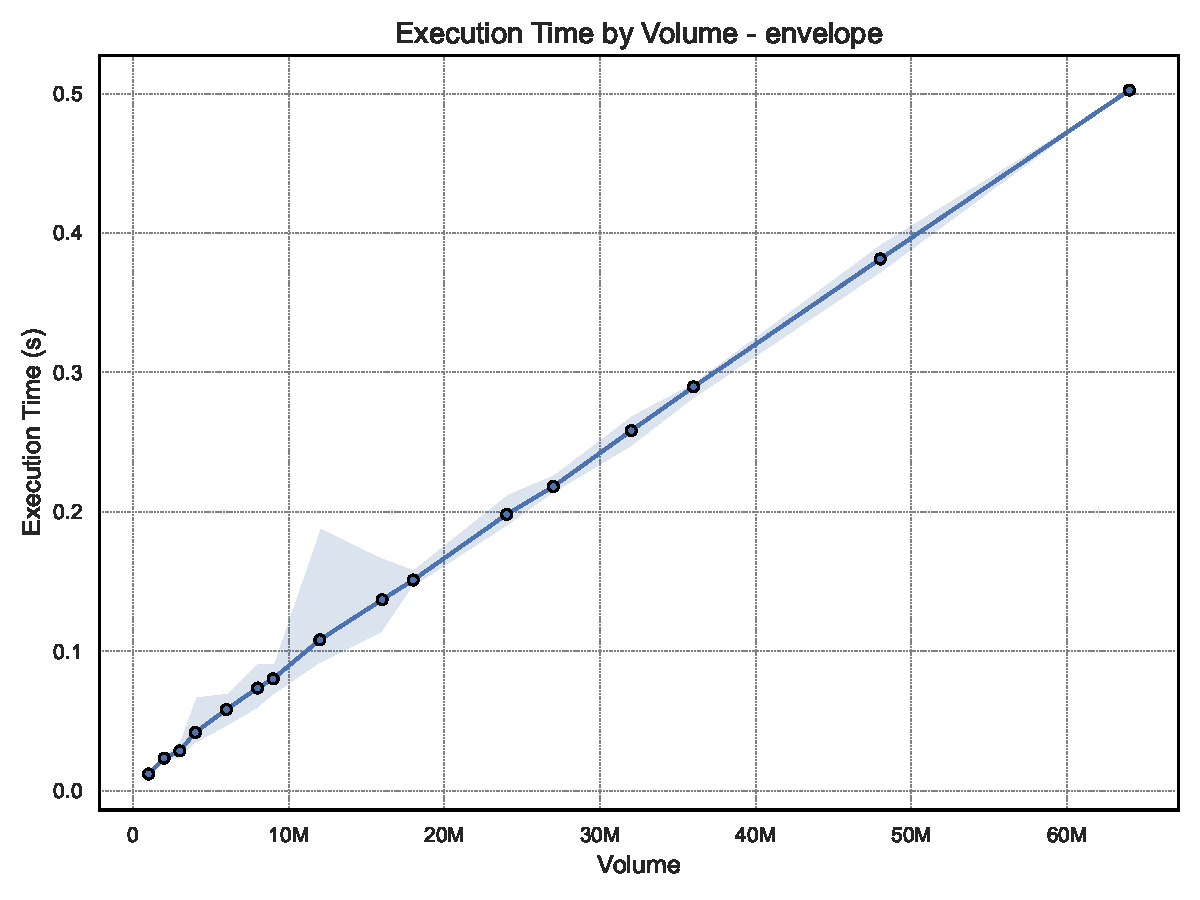
\includegraphics[width=\textwidth]{assets/images/05/execution_time_by_volume_envelope}
    \end{subfigure}
    \hfill
    \begin{subfigure}[t]{0.49\textwidth}
        \centering
        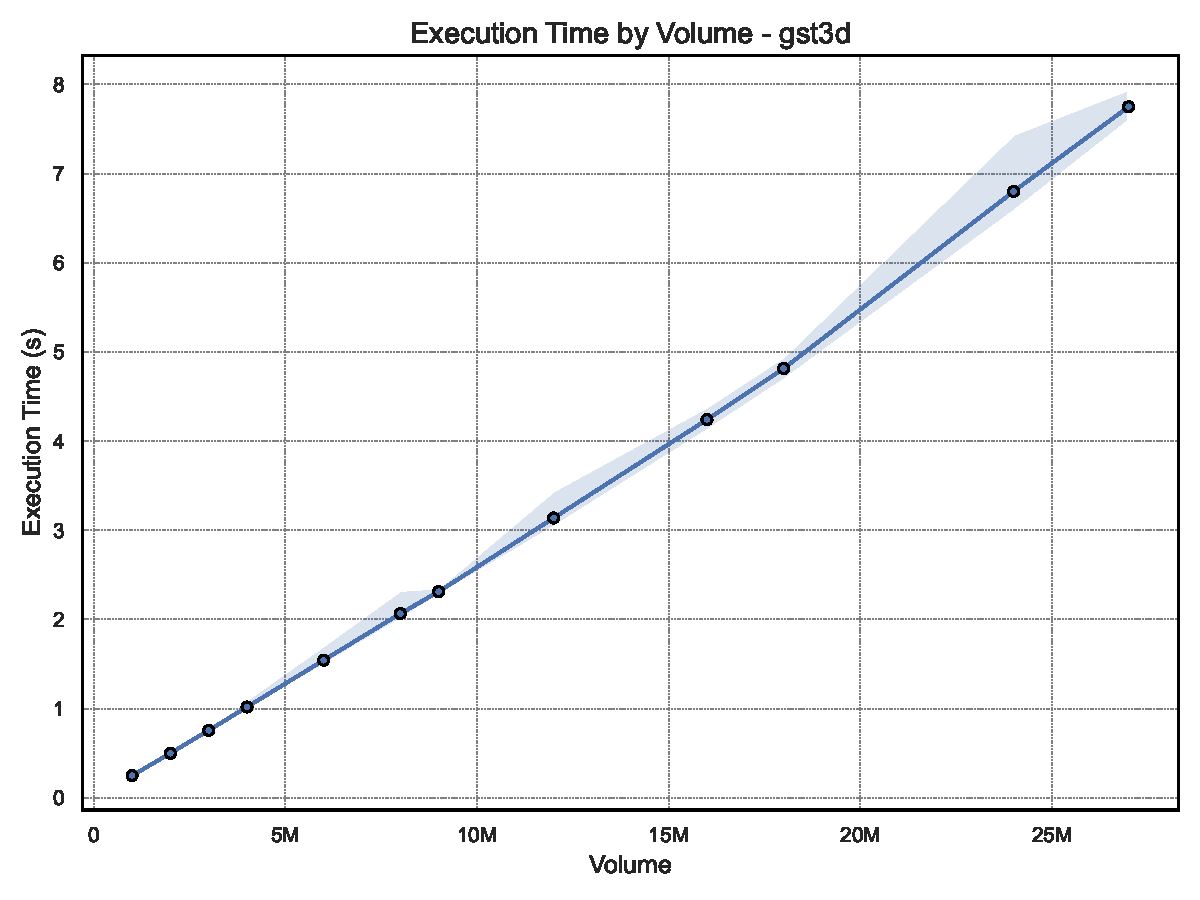
\includegraphics[width=\textwidth]{assets/images/05/execution_time_by_volume_gst3d}
    \end{subfigure}
    \hfill
    \begin{subfigure}[t]{0.49\textwidth}
        \centering
        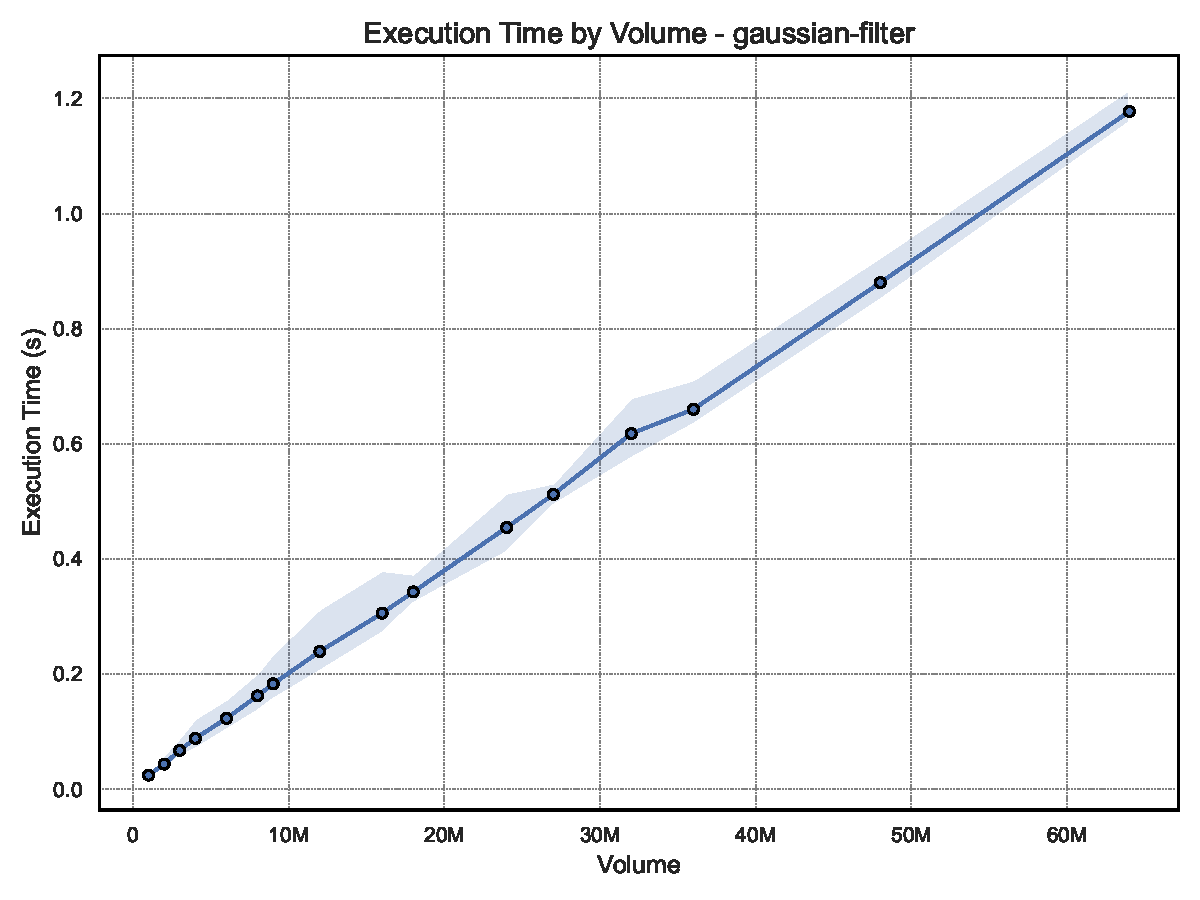
\includegraphics[width=\textwidth]{assets/images/05/execution_time_by_volume_gaussian-filter}
    \end{subfigure}
    \caption{
        Execution time by volume for Envelope, \ac{GST3D}, and Gaussian Filter. 
        All three operators show an increasing trend, reinforcing the impact of volume on processing duration. 
        \label{fig:execution_time_by_volume_facet}
    }
\end{figure*}

\subsection{Execution Time Distributions and Scaling Factor}
\label{subsec:execution-time-distributions-and-scaling}

To complement the volume-based analysis, Figures~\ref{fig:ex_peak_mu_facet}(a)--(b) compare execution time and peak memory usage across all operators.
Both metrics escalate in near-lockstep with input size.
Figure~\ref{fig:ex_peak_mu_facet}(c) then quantifies memory scaling slopes via linear-fits for each operator’s average peak \ac{RAM} usage. 
\EB{Acho que fica melhor mostrar o slope da regressão linear em uma tabela - você poderia mostrar o $R^2$ também. Isso tornadria o gráfico menor e talvez passível de inserção logo após o parágrafo que referencia ele.}
\ac{GST3D} stands out for having the highest slope, suggesting it holds more intermediate data structures during discontinuity detection.
Envelope lies in the middle, while Gaussian Filter’s slope is relatively smaller, implying that it processes data blocks \EBC{more incrementally}{o que quer dizer de forma mais incremental? seria por partes? Mas todos eles não realizam o cálculo por partes? i.e., por chunks?}.

\begin{figure*}[htbp]
    \centering
    \begin{subfigure}[t]{0.49\textwidth}
        \centering
        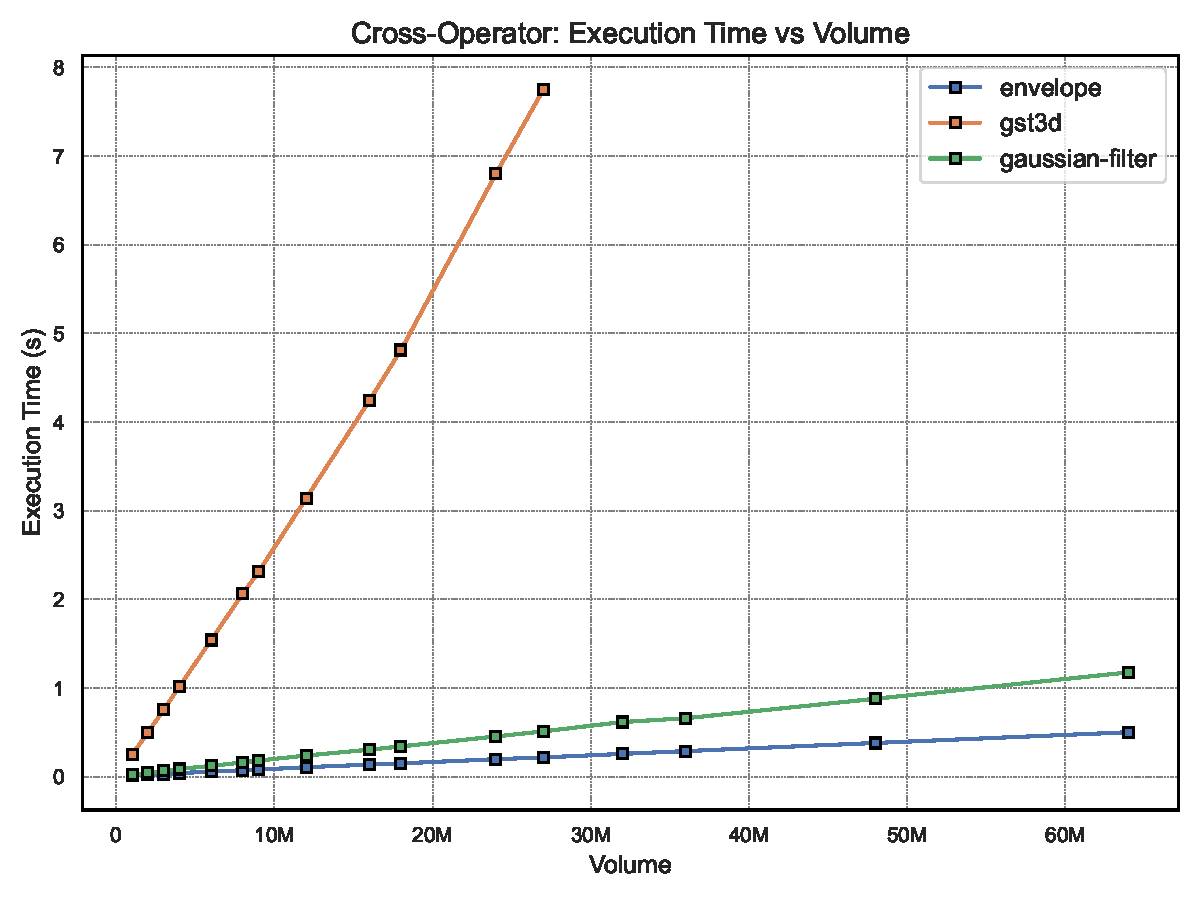
\includegraphics[width=\textwidth]{assets/images/05/cross_execution_time_by_volume}
        \caption{Execution time vs. volume for all three operators.}
    \end{subfigure}
    \hfill
    \begin{subfigure}[t]{0.49\textwidth}
        \centering
        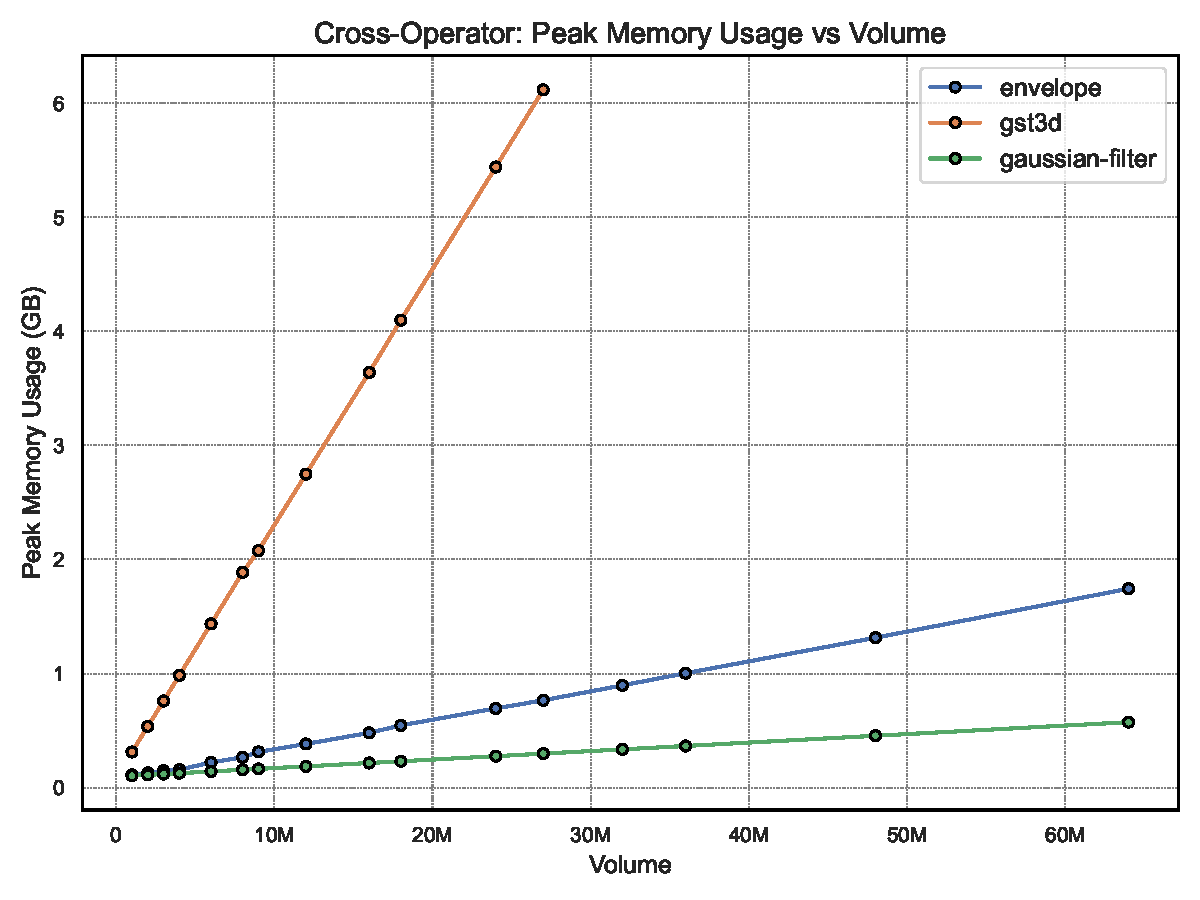
\includegraphics[width=\textwidth]{assets/images/05/cross_peak_memory_by_volume}
        \caption{Peak memory usage vs. volume for all three operators.}
    \end{subfigure}
    \hfill
    \begin{subfigure}[t]{0.49\textwidth}
        \centering
        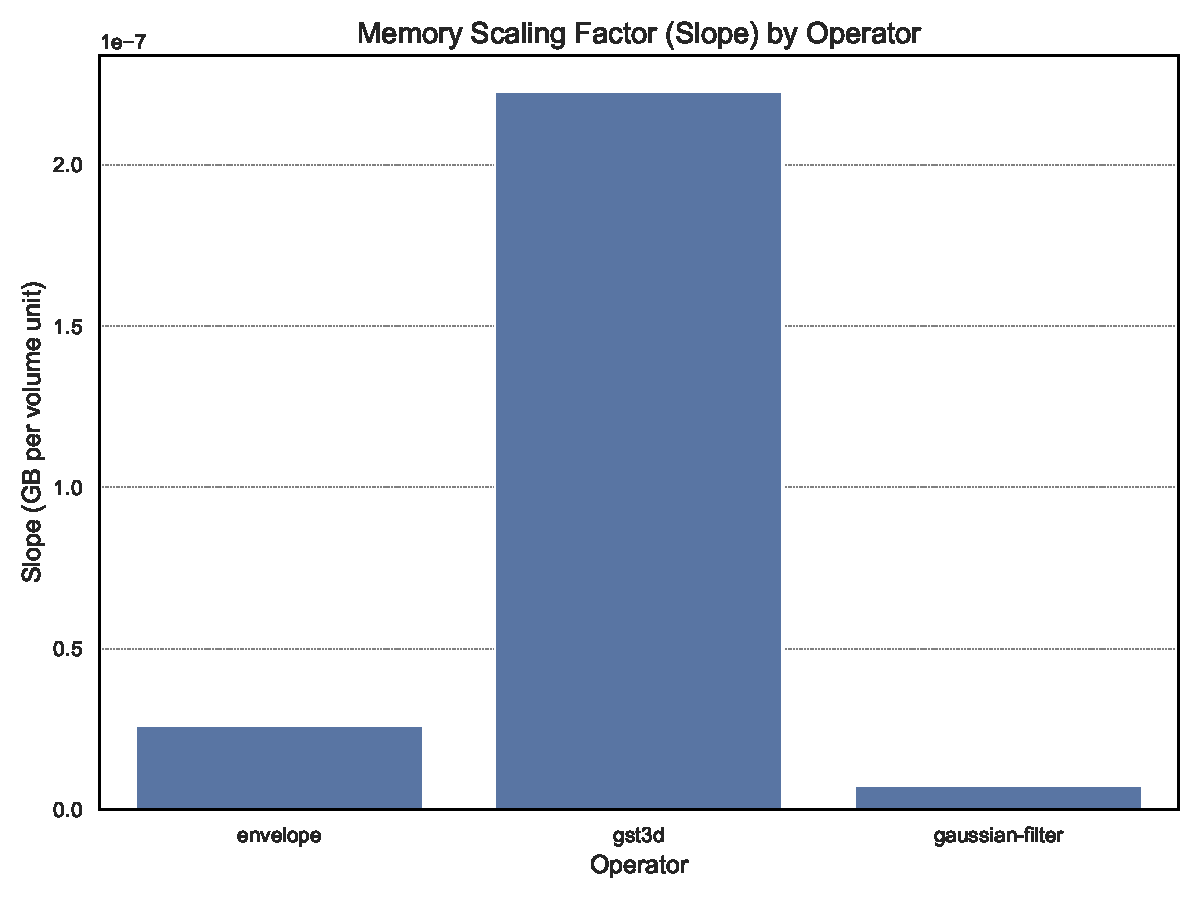
\includegraphics[width=\textwidth]{assets/images/05/cross_operator_memory_scaling_factor}
        \caption{
            Linear-fit slope values (GB/volume). Higher values indicate more pronounced memory growth.
            \EB{Como coloquei no texto, talvez fique melhor remover este gráfico daqui e colocar a informação em uma tabela.}
        }
    \end{subfigure}
    \caption{Combined view of execution time and peak memory usage by volume, and a bar chart revealing the linear-fit slopes for Envelope, \ac{GST3D}, and Gaussian Filter. \ac{GST3D} uses memory most aggressively, while Gaussian Filter is comparatively more memory efficient.}
    \label{fig:ex_peak_mu_facet}
\end{figure*}

In addition, the run durations exhibit right-skewed behavior (Figure~\ref{fig:execution_time_distribution_facet}), consistent with gamma- or lognormal-like distributions. \EB{Este gráfico mostra o histograma do tempo de execução de todos os experimentos? Variando o tamanho do dado? Se sim, a distribuição de tempo de execução tem uma relação mais forte com a seleção das amostras (tamanhos) do que com ruído no sistema, certo?}
While most executions concentrate in the lower range, occasional runs can be significantly longer.
Such tails are not unexpected in \ac{HPC} environments, where system-level noise or particular dataset structures can cause prolonged I/O or memory allocation overhead.
\EB{Não está claro pra mim como este gráfico e estes resultados de tempo contribuem para as principais conclusões derivadas neste capítulo. É interessante ter uma noção do tempo de execução, até mesmo para saber o custo de ser realizar estes experimentos e/ou coletar dados para treinar os modelos, mas além deste ponto, não sei se uma análise de correlação de features e/ou consumo de memória com o tempo de execução está dando suporte aos principais argumentos ou poluindo o capítulo.}

\begin{figure*}[htbp]
    \centering
    \begin{subfigure}[t]{0.49\textwidth}
        \centering
        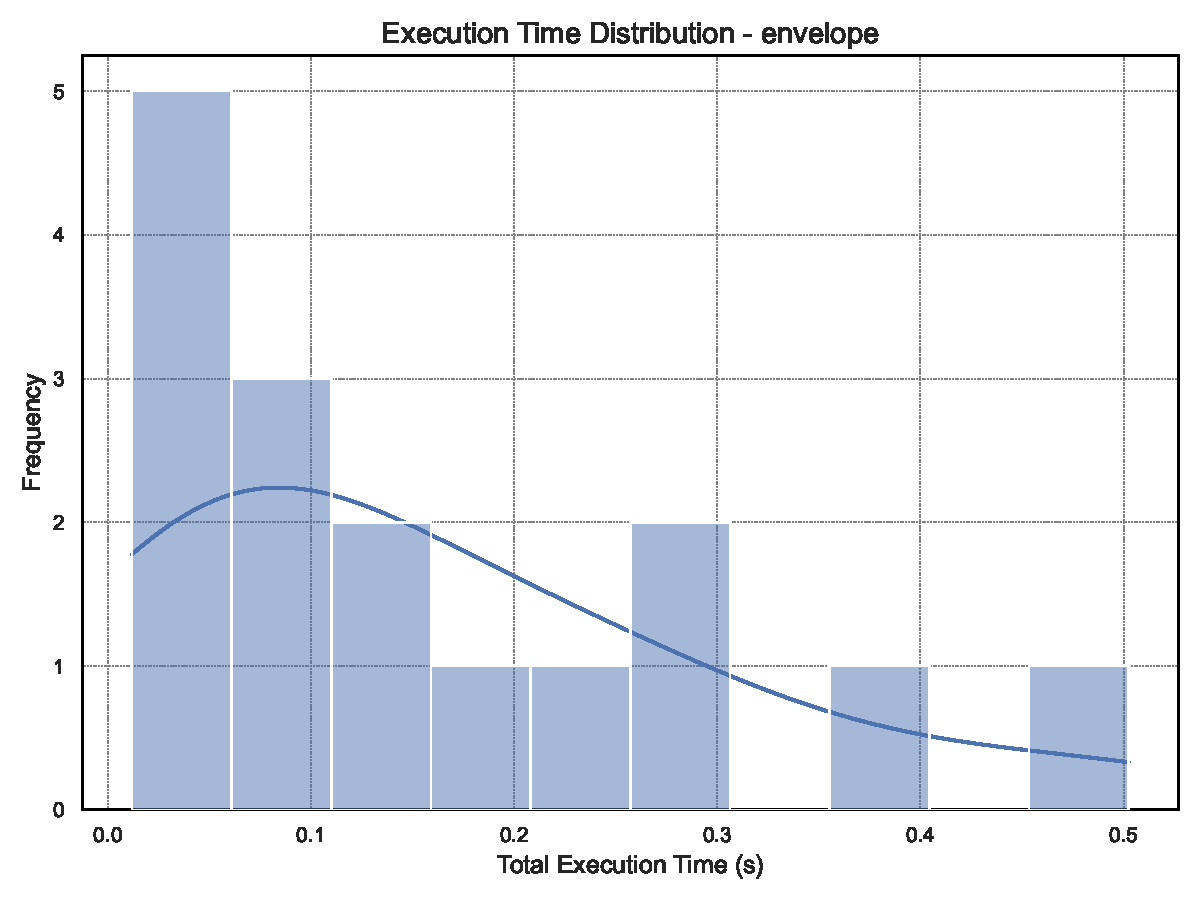
\includegraphics[width=\textwidth]{assets/images/05/execution_time_distribution_envelope}
    \end{subfigure}
    \hfill
    \begin{subfigure}[t]{0.49\textwidth}
        \centering
        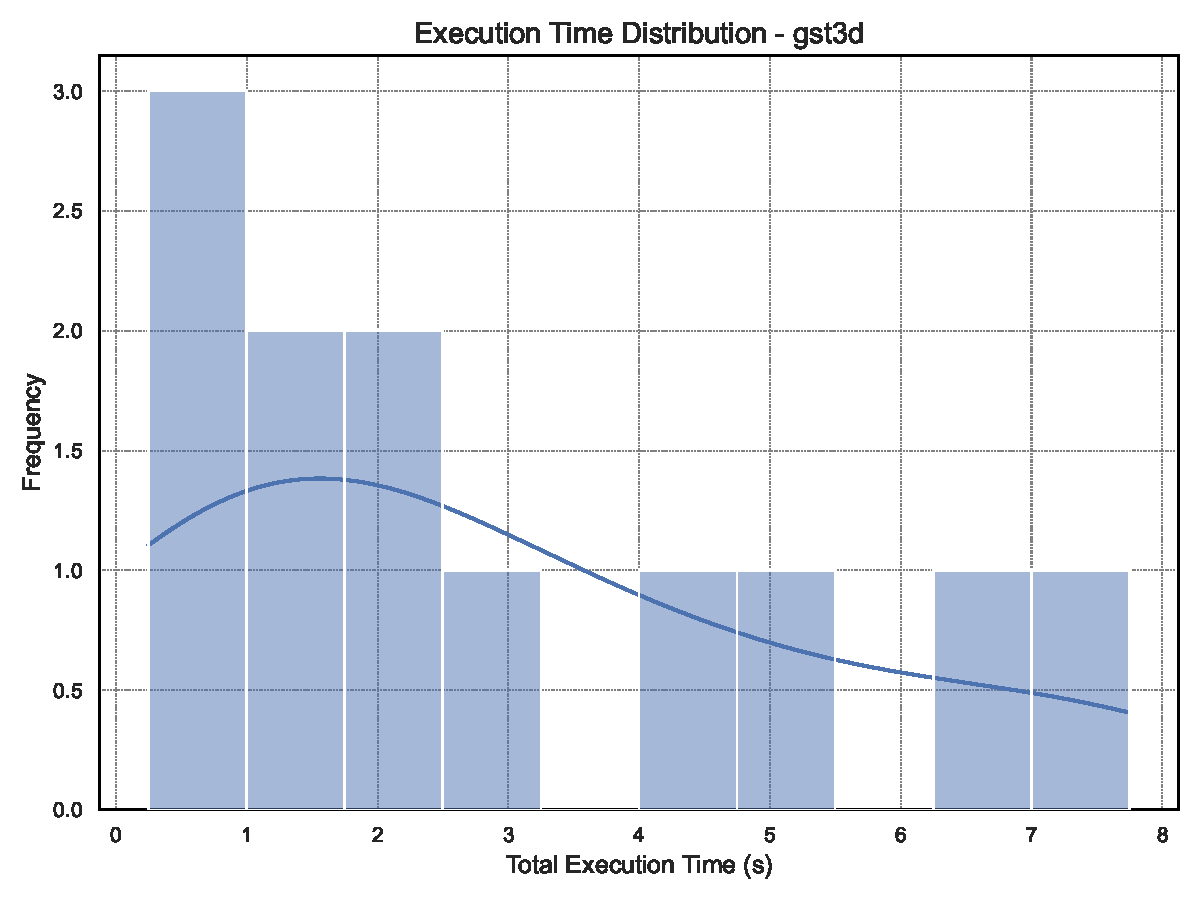
\includegraphics[width=\textwidth]{assets/images/05/execution_time_distribution_gst3d}
    \end{subfigure}
    \hfill
    \begin{subfigure}[t]{0.49\textwidth}
        \centering
        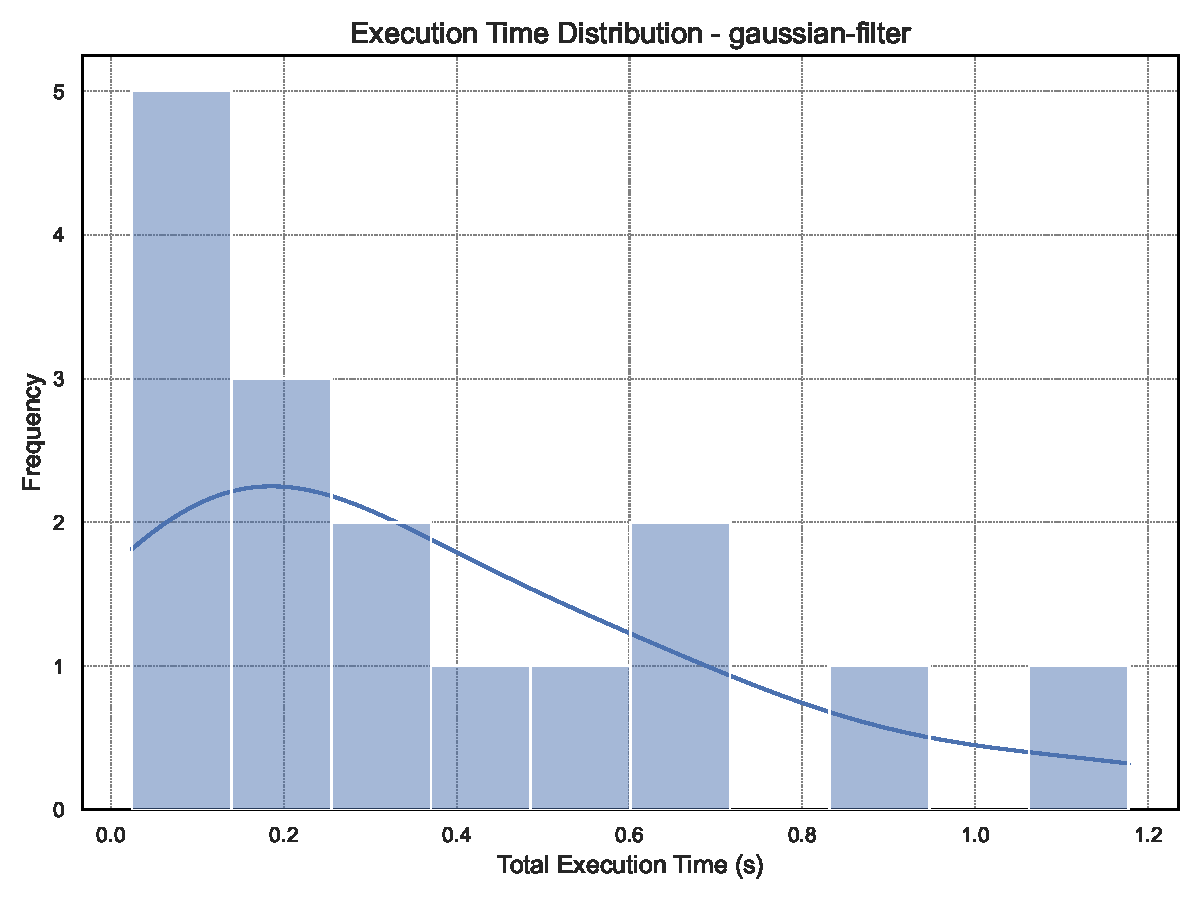
\includegraphics[width=\textwidth]{assets/images/05/execution_time_distribution_gaussian-filter}
    \end{subfigure}
    \caption{Execution time distributions for Envelope, \ac{GST3D}, and the Gaussian Filter. Each distribution displays a heavy right tail, indicating that while most runs finish quickly, certain configurations or system conditions can cause notable slowdowns.}
    \label{fig:execution_time_distribution_facet}
\end{figure*}

\subsection{Dimension-Specific and Time-Progression Analysis}
\label{subsec:dimension-specific-and-time-progression-analysis}

\EB{Como mencionei anteriormente, não está claro para mim se esta análise de tempo de execução é muito relevante.}

To better understand how different axes of the seismic volume factor into resource usage, we break down memory usage by \emph{inlines}, \emph{xlines}, and \emph{samples} for the Envelope operator~(Figure~\ref{fig:memory_usage_by_configuration_envelope}).
We observe that each dimension exerts a similar influence on memory consumption; no single dimension overwhelmingly dominates the Envelope’s consumption pattern.
This outcome aligns with the notion that Envelope is an element-wise amplitude calculation, depending uniformly on the size of the entire input array.

\begin{figure*}[htbp]
    \centering
    \begin{subfigure}[t]{0.49\textwidth}
        \centering
        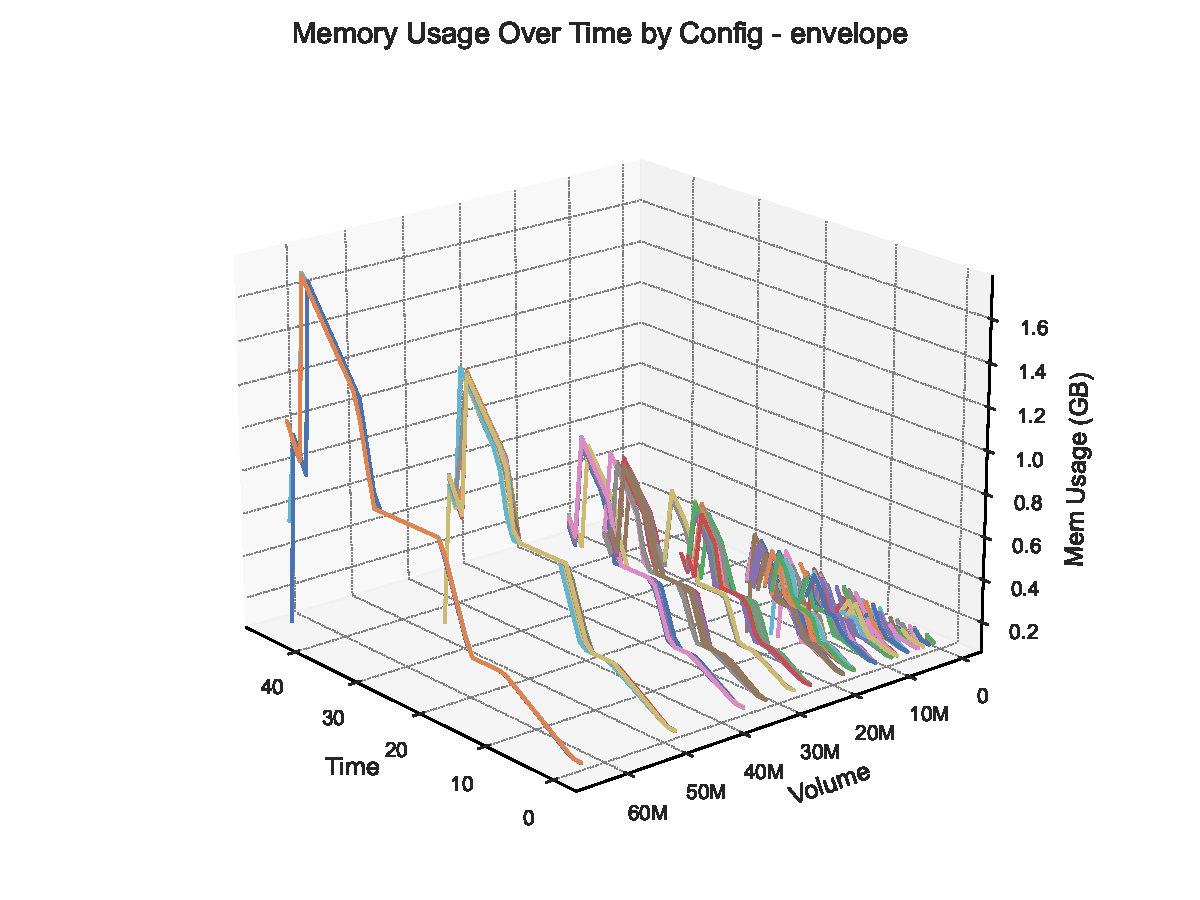
\includegraphics[width=\textwidth]{assets/images/05/memory_usage_by_configuration_envelope}
        \caption{Memory usage binned by individual shape parameters. Each axis increases overall memory similarly.}
    \end{subfigure}
    \hfill
    \begin{subfigure}[t]{0.49\textwidth}
        \centering
        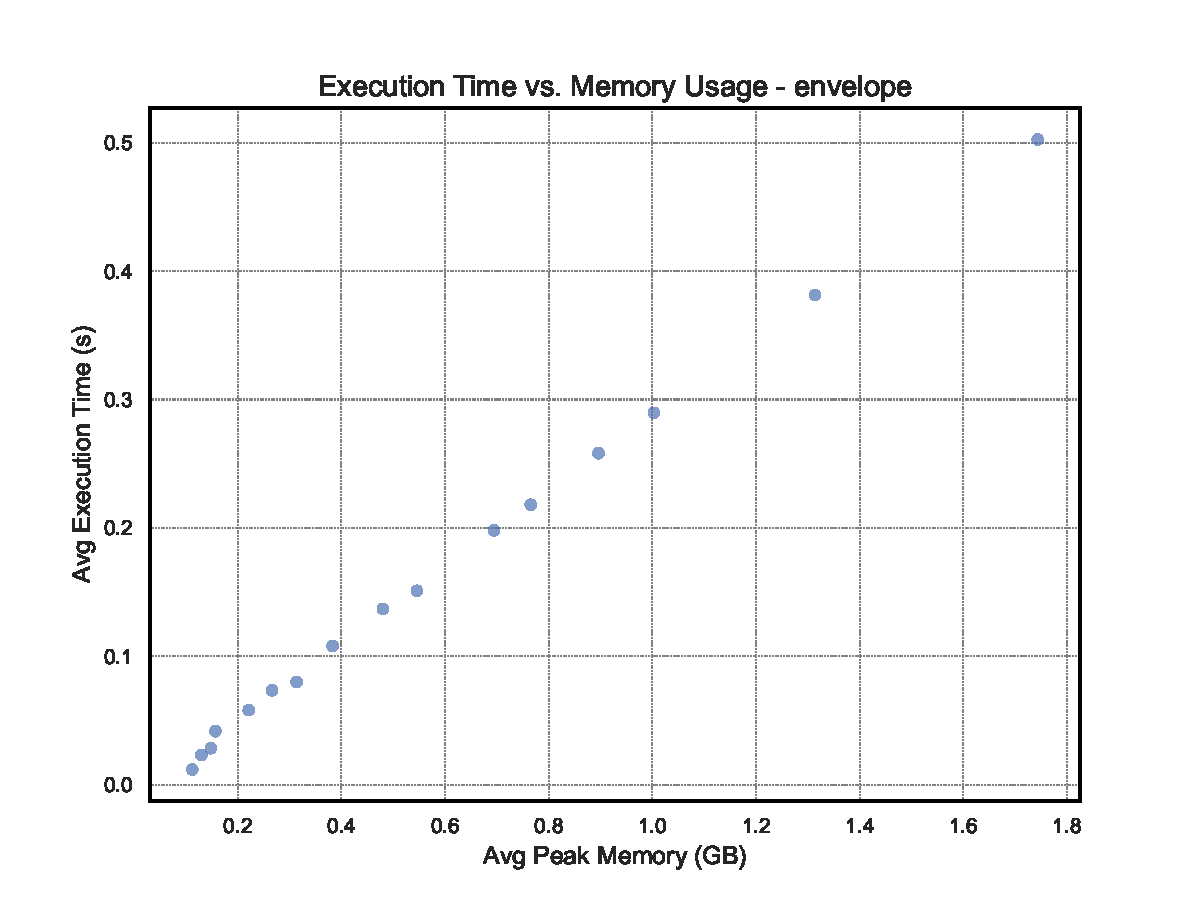
\includegraphics[width=\textwidth]{assets/images/05/execution_time_vs_memory_envelope}
        \caption{Execution time vs. memory usage for Envelope, indicating a mild correlation (longer runs often consume more \ac{RAM}).
            \EB{Não ficou claro para mim como este resultado dá suporte às principais conclusões do capítulo.}
        }
    \end{subfigure}
    \hfill
    \begin{subfigure}[t]{0.49\textwidth}
        \centering
        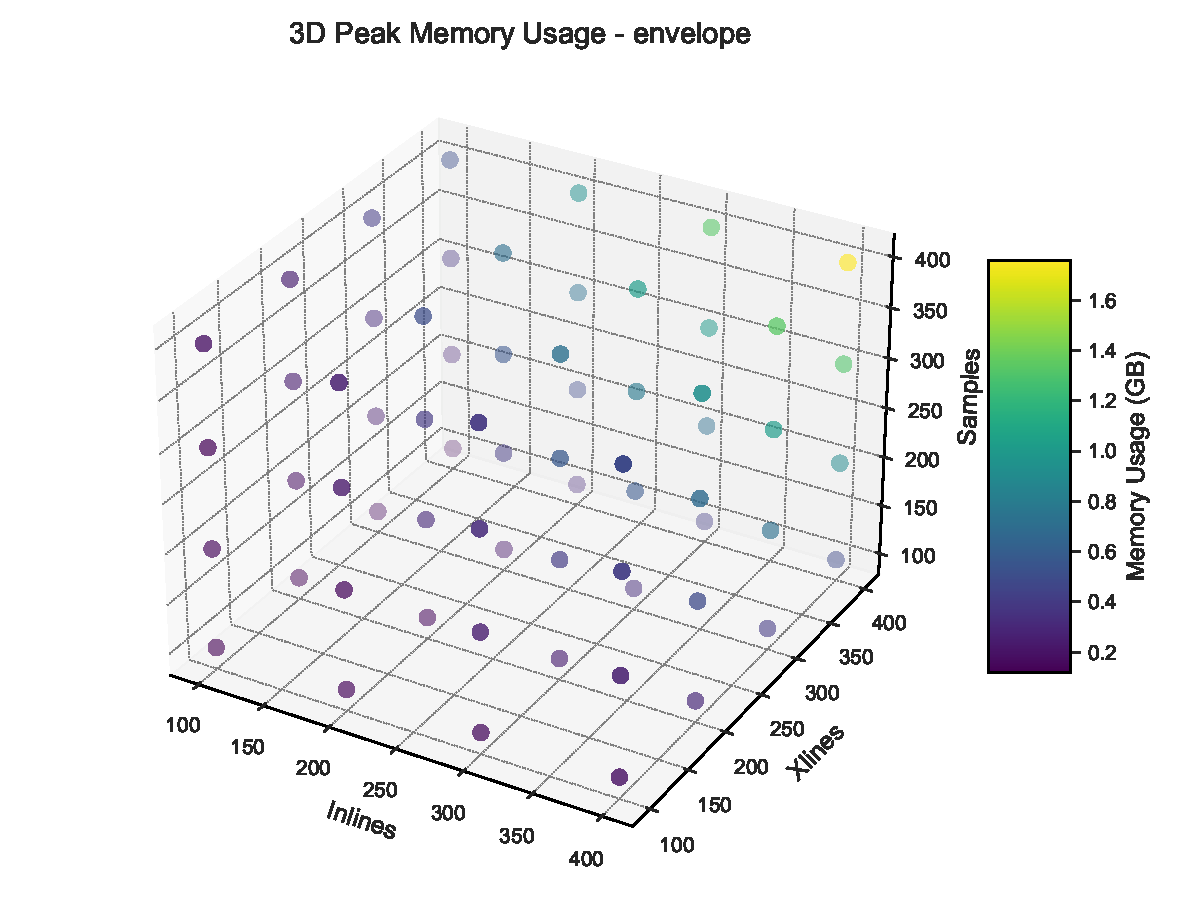
\includegraphics[width=\textwidth]{assets/images/05/memory_usage_inlines_xlines_samples_heatmap_envelope}
        \caption{Heatmap combining inlines, xlines, and samples into a 2D view; warmer colors indicate higher memory usage.
            \EB{Estou inferindo que o objetivo deste gráfico é mostrar que cada dimensão tem uma influência similar no consumo de memória. Se for o caso, acho que seria bom explicar o gráfico no texto e discutir quais características do gráfico levam a esta conclusão.}
        }
    \end{subfigure}
    \caption{Memory usage and runtime analysis for the Envelope operator. 
        All three dimensions appear to scale memory demand in a similar manner, and bigger shapes generally require longer processing times.
        \label{fig:memory_usage_by_configuration_envelope}
    }
\end{figure*}

Figure~\ref{fig:inline_xline_memory_usage_progression_envelope} further highlights how the Envelope operator’s memory usage accumulates over time.
The growth pattern is relatively uniform, aligning with the straightforward element-wise nature of the algorithm.
More complex operators like \ac{GST3D} may reveal steeper or stage-based ramps, particularly if certain algorithmic phases allocate additional buffers or caching mechanisms at specific intervals.
\EB{Qual a principal conclusão (\textit{insight}) que podemos derivar deste experimento?}

\begin{figure}[htbp]
    \centering
    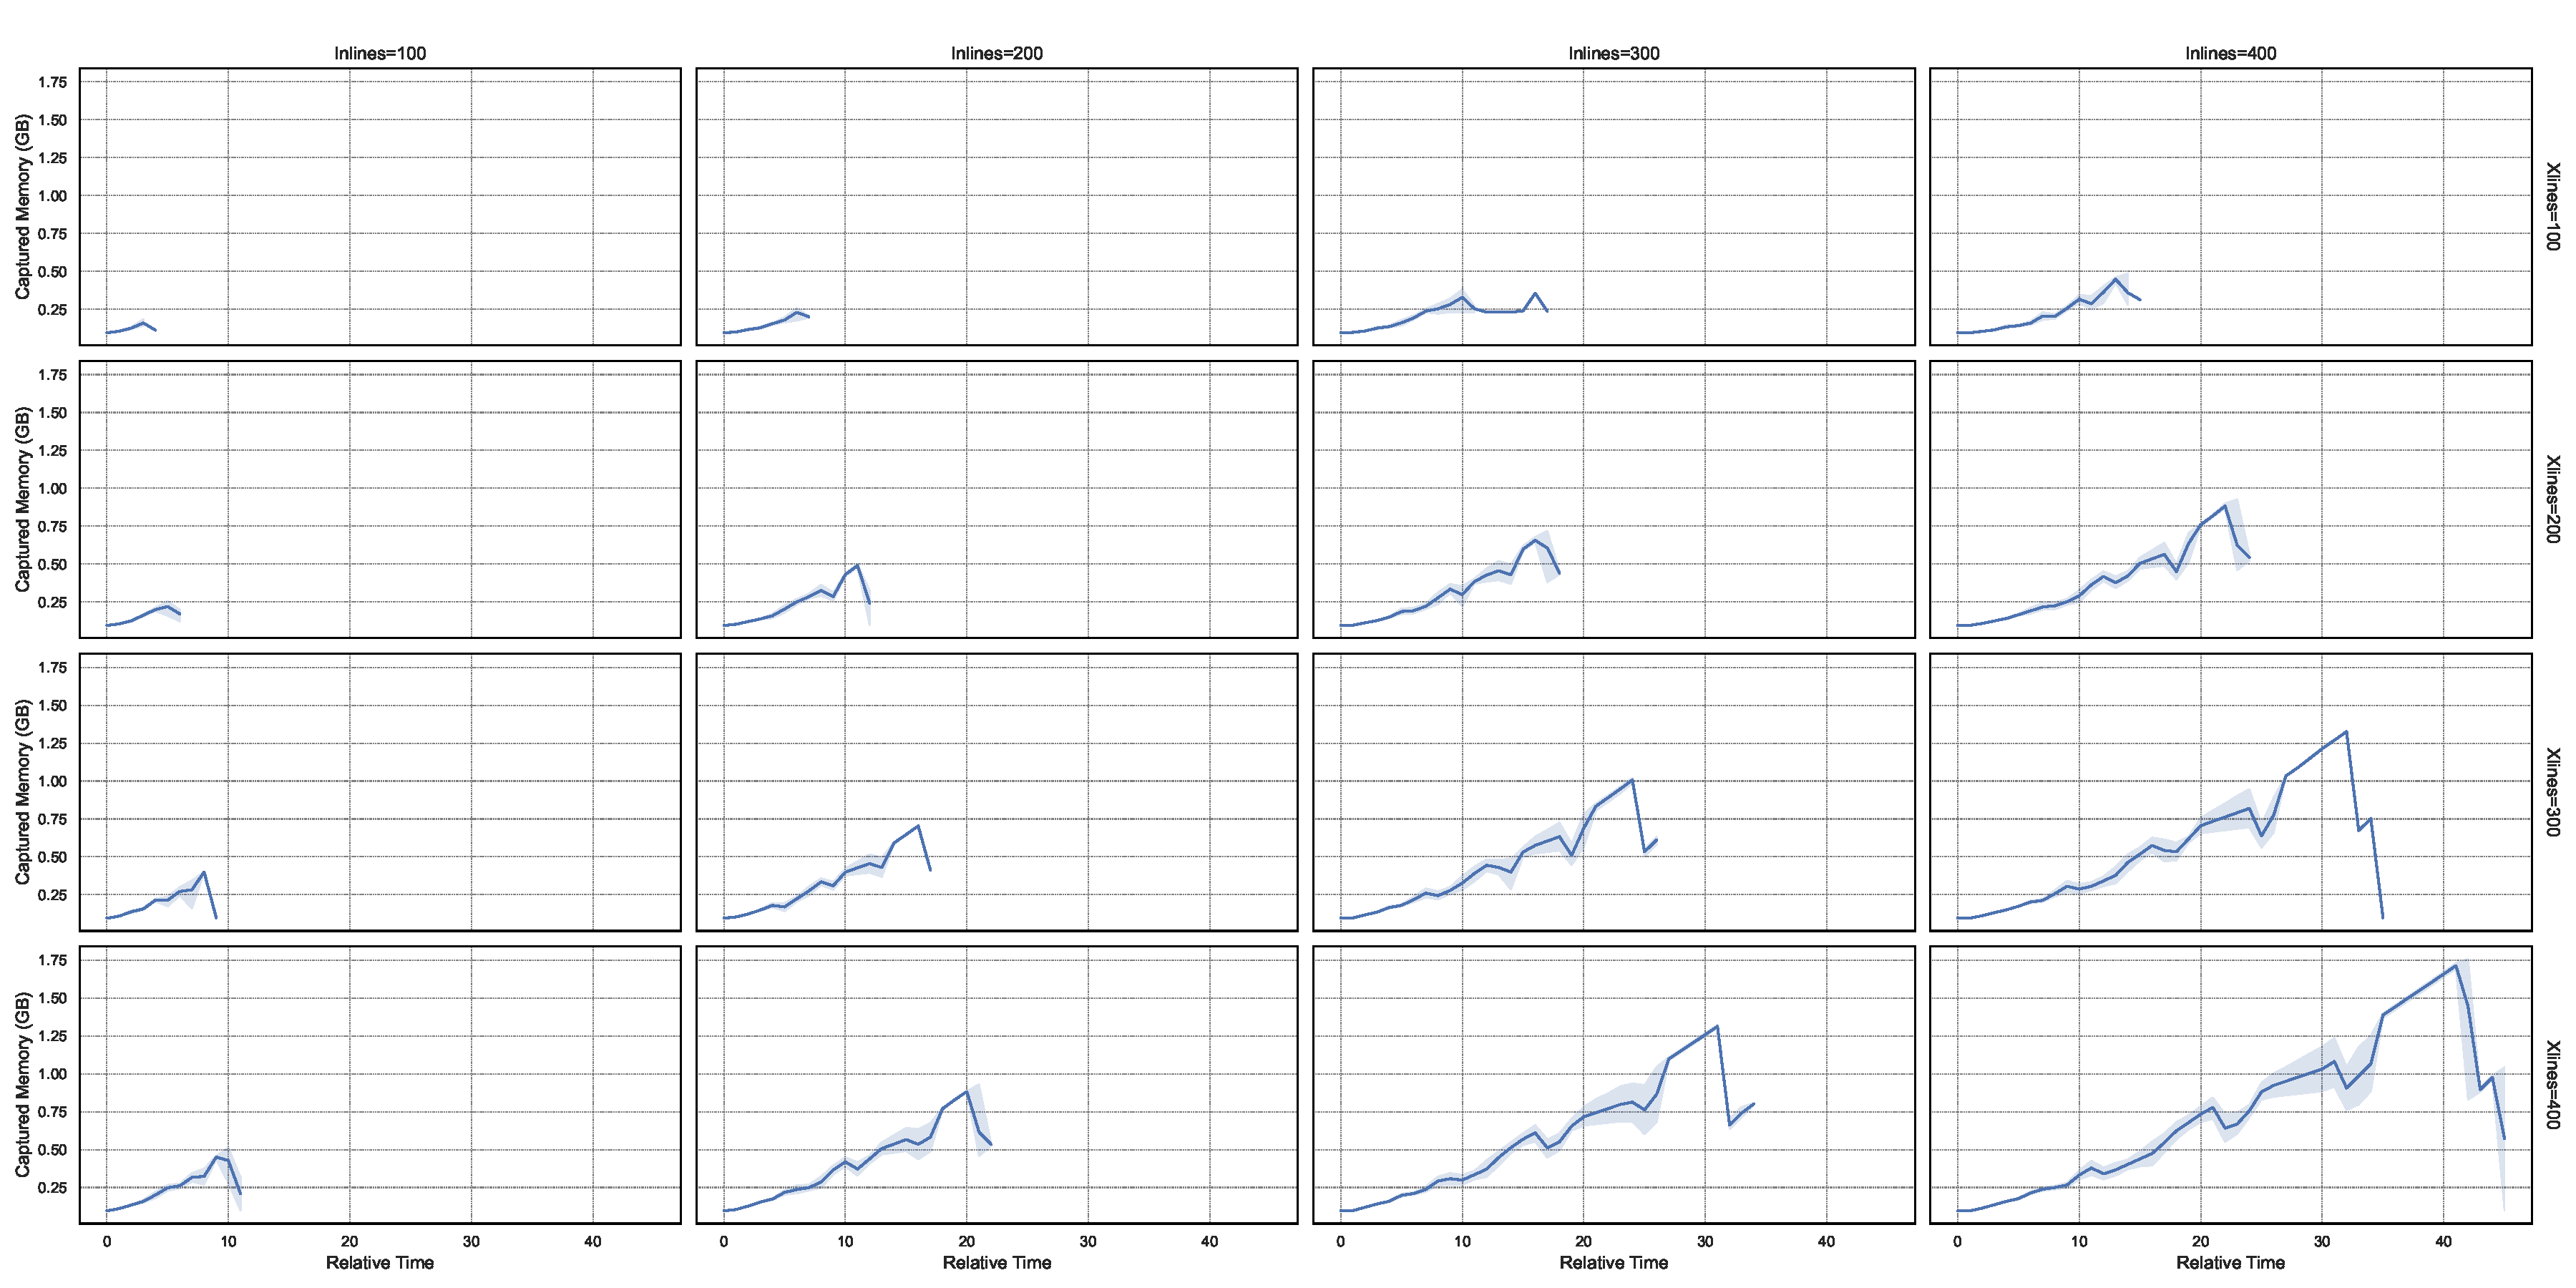
\includegraphics[width=\textwidth]{assets/images/05/inline_xline_memory_usage_progression_envelope}
    \caption{Memory usage progression over time (Envelope operator) for different inlines and xlines. 
        The consumption profile ramps up gradually rather than spiking in distinct phases.
        \label{fig:inline_xline_memory_usage_progression_envelope}
    }
\end{figure}

\subsection{Memory Safety Margins}
\label{subsec:memory-safety-margins}

In real-world \ac{HPC} contexts, underestimating memory can cause abrupt job failures, while overestimation wastes resources.
Figure~\ref{fig:memory_safety_margin} showcases how much peak usage can deviate from average usage by comparing mean and 95th-percentile values.
Envelope and \ac{GST3D} exhibit particularly large deviations for certain volume ranges, hinting that HPC practitioners may need to add a safety buffer beyond the mean consumption to accommodate transient memory spikes.
\EB{Este parágrafo me leva a crer que você está usando a \emph{feature} volume para fazer esta análise. Não seria mais adequado agrupar os dados de acordo com a tupla (inlines, xlines, samples) para evitar que variações de consumo de memória causadas por mudanças nestes valores nos levem a concluir que o motivo é o sistema? P.ex., a tupla (10, 10, 20) pode gerar resultados da tupla (20, 10, 10) que, apesar de terem o mesmo volume, são diferentes.}
\EB{Se tem tanta variação, como foi possível treinar os modelos somente com esta feature e chegar a valores de erro tão pequenos? Os erros não deveriam refletir as variações que observamos aqui?}


\begin{figure*}[htbp]
    \centering
    \begin{subfigure}[t]{0.49\textwidth}
        \centering
        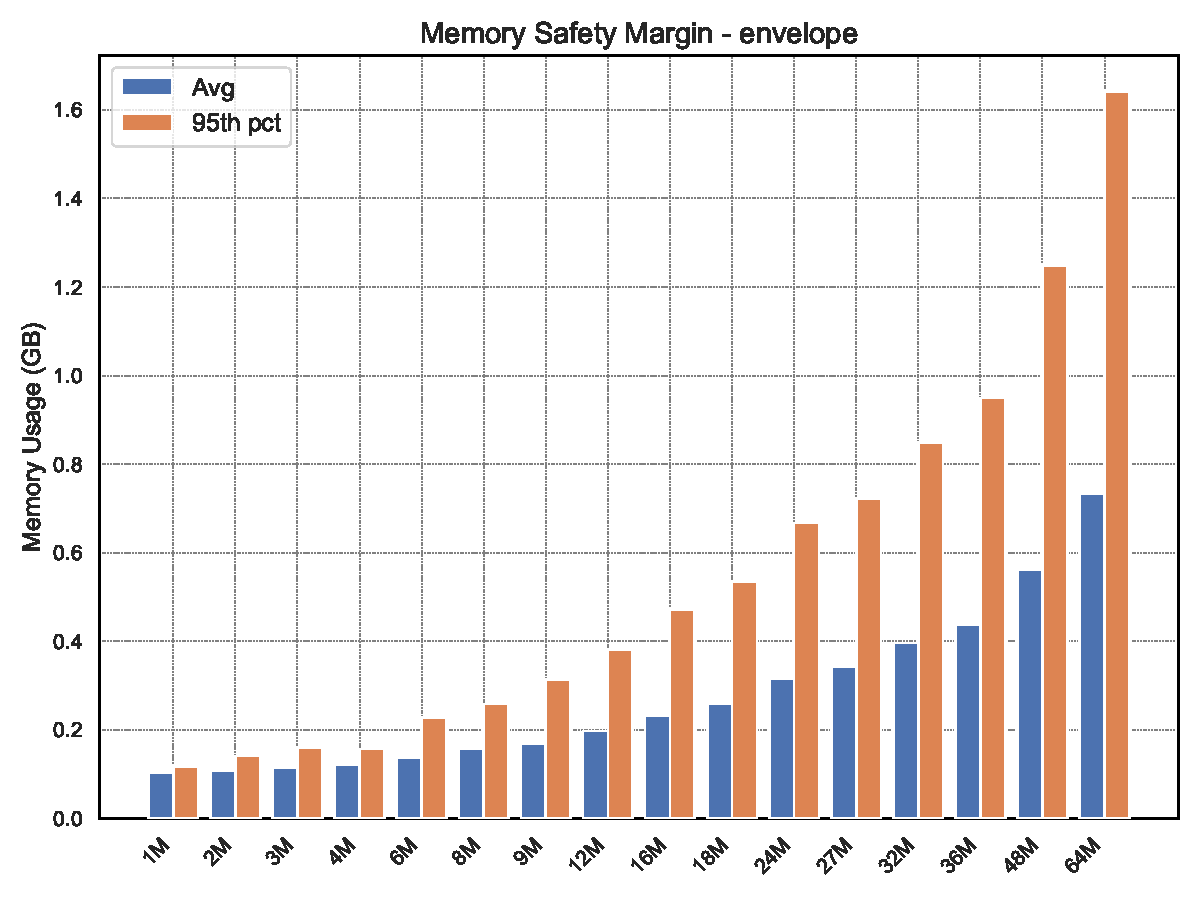
\includegraphics[width=\textwidth]{assets/images/05/memory_safety_margin_envelope}
    \end{subfigure}
    \hfill
    \begin{subfigure}[t]{0.49\textwidth}
        \centering
        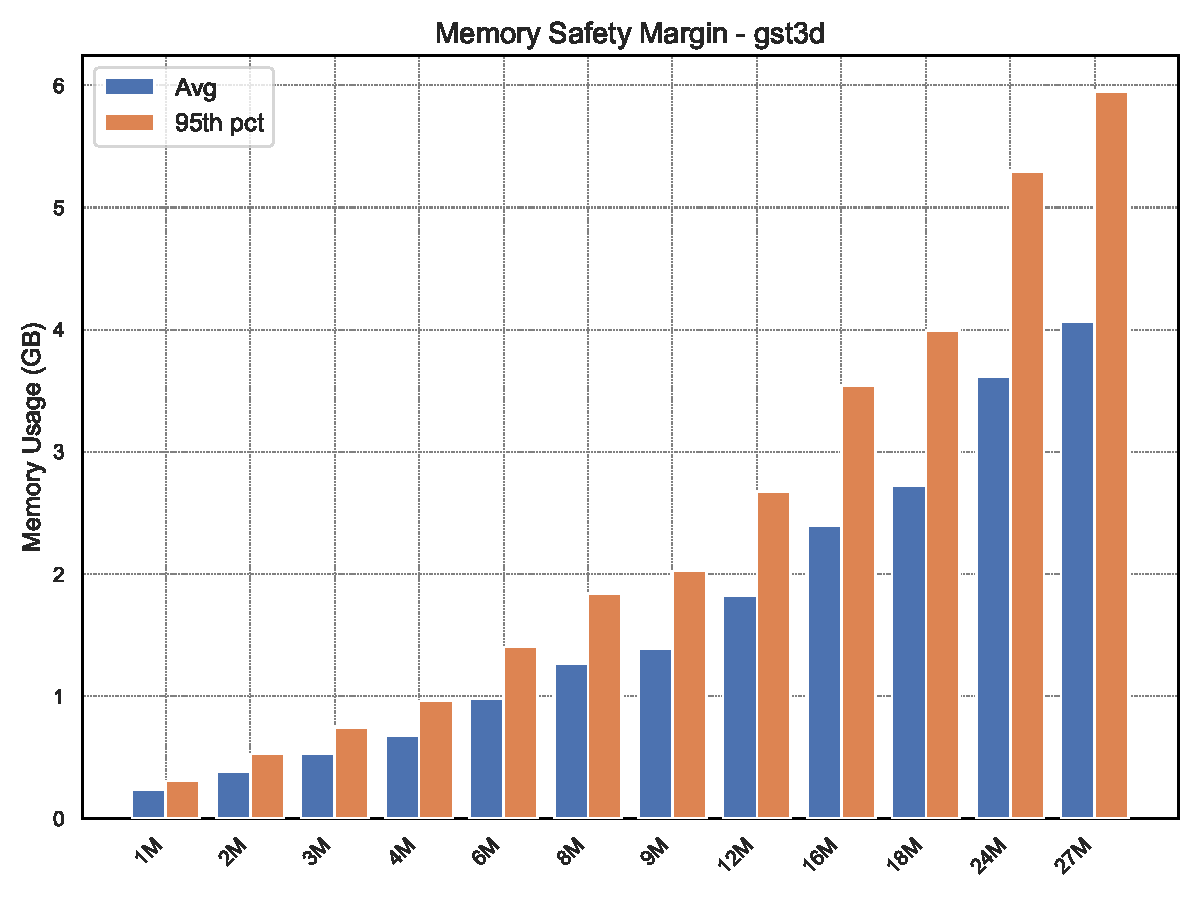
\includegraphics[width=\textwidth]{assets/images/05/memory_safety_margin_gst3d}
    \end{subfigure}
    \hfill
    \begin{subfigure}[t]{0.49\textwidth}
        \centering
        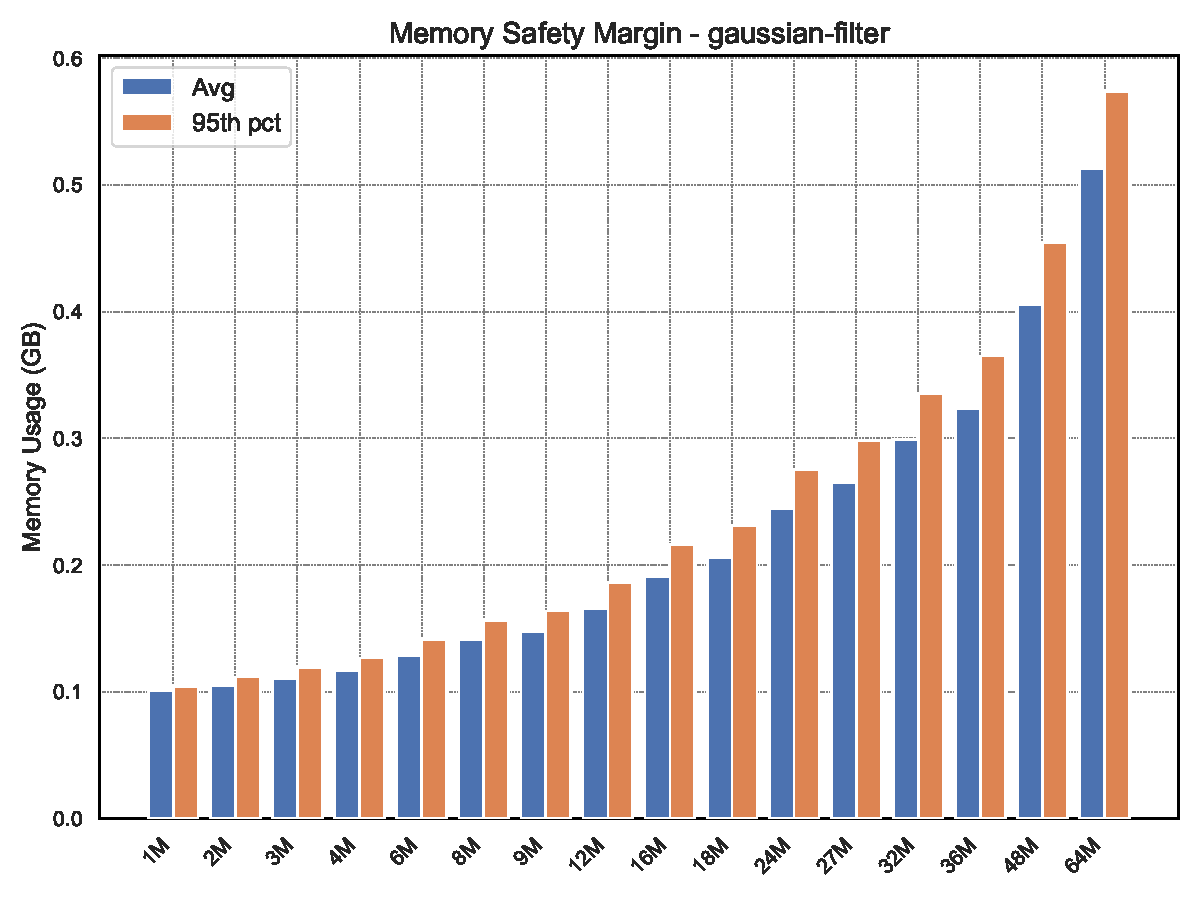
\includegraphics[width=\textwidth]{assets/images/05/memory_safety_margin_gaussian-filter}
    \end{subfigure}
    \caption{Memory safety margins for Envelope, \ac{GST3D}, and the Gaussian Filter. The 95th-percentile often surpasses mean usage by a noticeable margin, revealing the unpredictability of peak memory events.}
    \label{fig:memory_safety_margin}
\end{figure*}

These outliers can arise from transient allocation bursts, system-level scheduling, or overhead fluctuations.
Even with container-based isolation, kernel-level memory management can introduce sporadic spikes.
Recognizing these high-percentile events is critical for designing robust pre-runtime memory estimators.
If left unaccounted for, such transient peaks could lead to underestimation, especially for borderline volumes.

\EB{Este me parece ser uma seção bem importante, já que ela discute a questão da margem de erro que devemos levar em consideração na avaliação dos modelos. Quando trabalhamos com os modelos estamos utilizando dados baseados na média ou no 95\%?} 
\EB{Para refletir: Será que não deveríamos estar usando os dados crus, e monitorar estas variações nos errors?}

\EB{BTW, esta variabilidade é usada no cálculo do score que você menciona nas seções subsequentes?}

\subsection{Dimension Correlations}
\label{subsec:dimension-correlations}

We can further investigate how dimension-specific growth patterns contribute to overall memory usage by plotting pairwise relationships between memory usage and the three shape parameters.
Figure~\ref{fig:memory_vs_dimensions_pairplot_gst3d} shows that \ac{GST3D}, in particular, has strong positive correlations between each dimension and peak memory.
Meanwhile, dimension--dimension scatter plots sometimes show inverse correlations due to the systematic way shapes were varied (when one axis is large, another might be slightly smaller).
Nevertheless, once all three dimensions expand simultaneously, the net memory usage grows sharply.

\EB{Daniel, não entendi o gráfico. O que significam os pontos azuis e as linhas vermelhas?}

\begin{figure}[htbp]
    \centering
    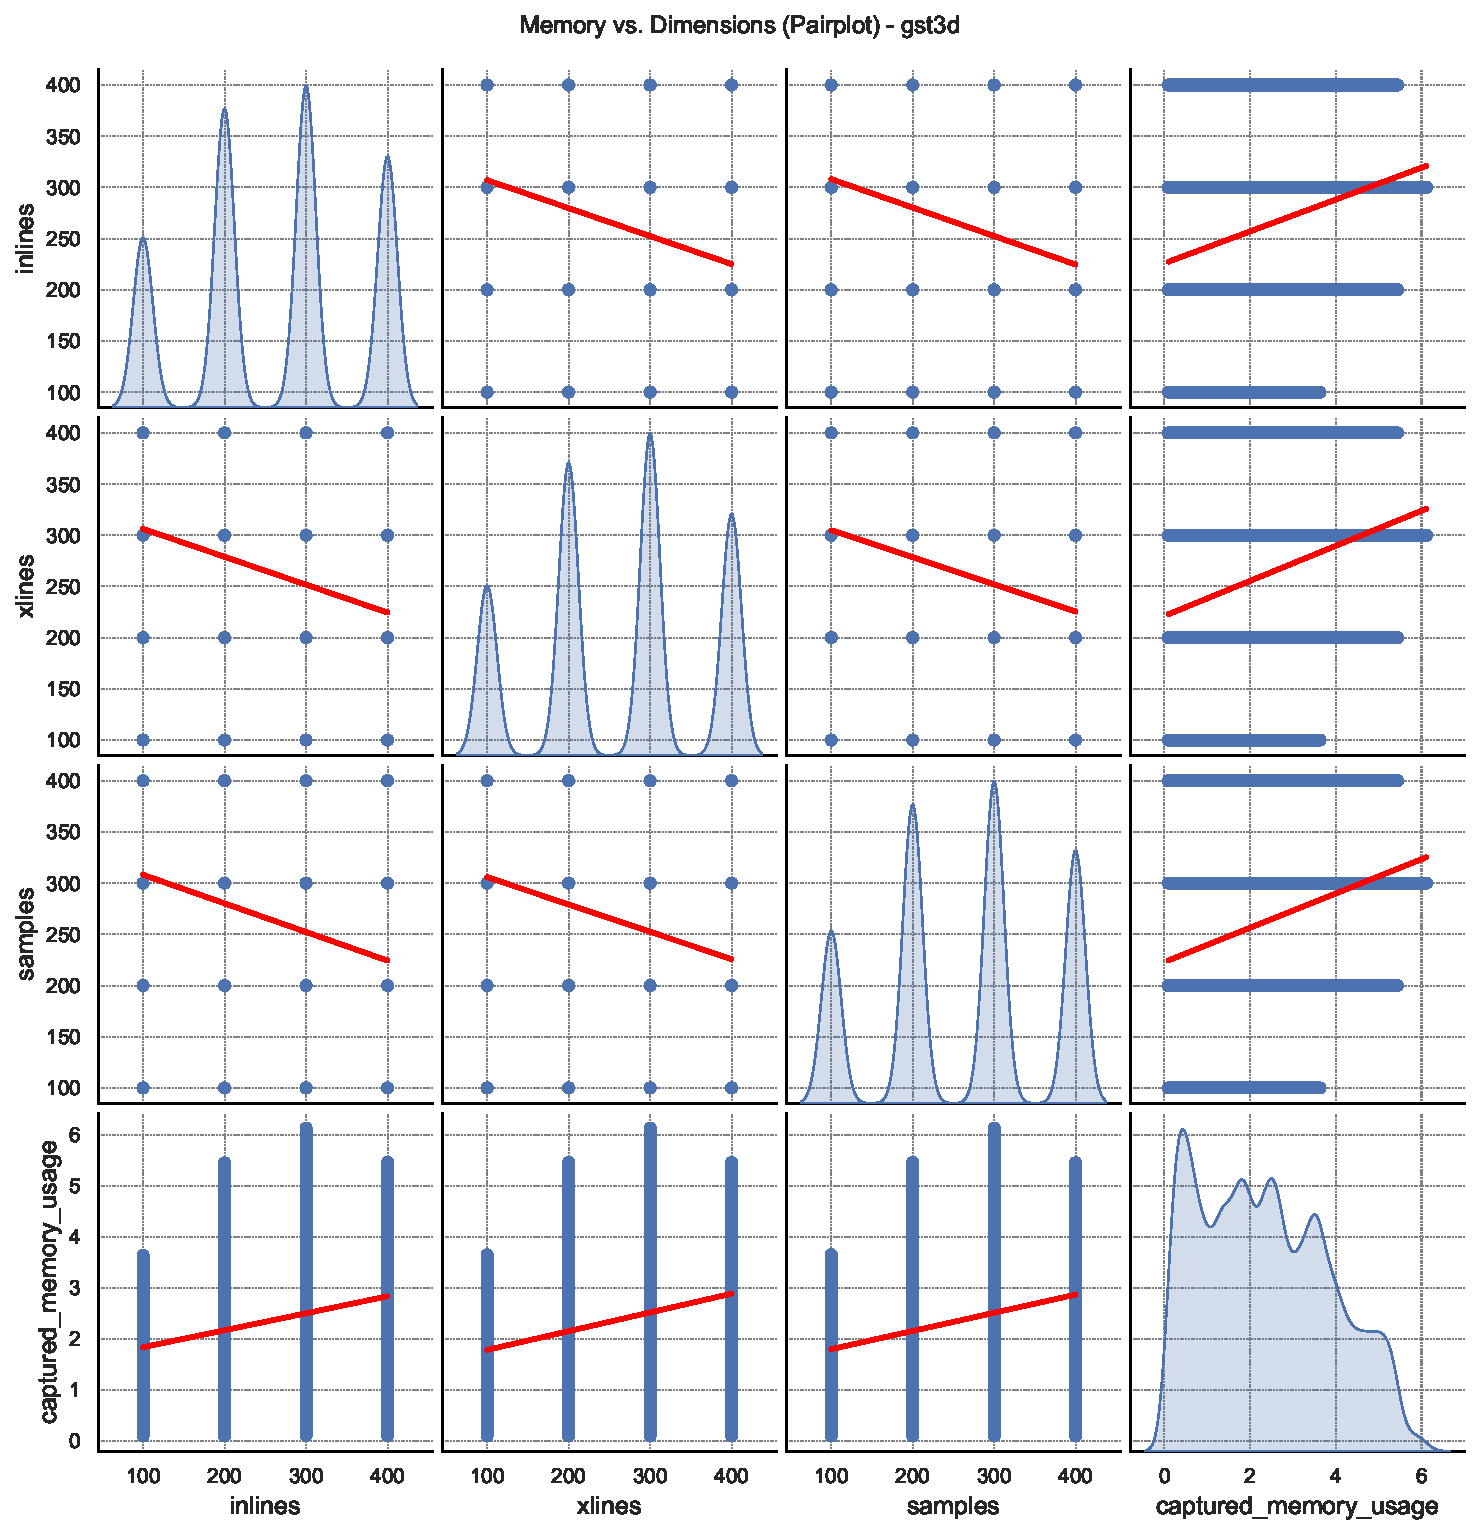
\includegraphics[width=0.9\textwidth]{assets/images/05/memory_vs_dimensions_pairplot_gst3d}
    \caption{Pairplot for \ac{GST3D} memory usage against inlines, xlines, and samples. Positive slopes in memory-related plots confirm that larger shape parameters escalate the overall memory footprint.}
    \label{fig:memory_vs_dimensions_pairplot_gst3d}
\end{figure}

These pairwise correlations, combined with the linear volume trend, underscore that each dimension matters and that polynomial or interaction-based features can help capture how memory usage evolves in less trivial cases (e.g., operators whose complexity grows nonlinearly along certain axes).
\EB{Não ficou claro para mim como você chegou nesta conclusão.}

\subsection{Summary of Observed Resource Usage}
\label{subsec:resource-usage-summary}

Table~\ref{tab:operator_summary_aggregates} provides a high-level summary of all tested volume ranges, memory usage spans, and measured execution times for each operator.
It highlights how, for similarly sized volumes, \ac{GST3D} consistently demands the greatest \EBADD{amount of} \ac{RAM}, with Envelope requiring intermediate amounts, and Gaussian Filter at the lower end (though still significant).
Processing times echo these patterns, with more complex or data-hungry operations tending to take longer.

\begin{table}[htbp]
    \centering
    \begin{tabular}{lcccc}
        \hline
        \textbf{Operator} & \textbf{Volume Range} & \textbf{Peak Mem. Usage (GB)} & \textbf{Exec. Time (s)} \\ \hline
        Envelope &
        $10^6 \!\to\! 6.4\times10^7$ &
        0.10 -- 1.76 &
        0.0106 -- 0.5025 \\
        \ac{GST3D} &
        $10^6 \!\to\! 2.7\times10^7$ &
        0.31 -- 6.12 &
        0.2475 -- 7.75 \\
        Gaussian Filter &
        $10^6 \!\to\! 6.4\times10^7$ &
        0.10 -- 0.57 &
        0.0232 -- 1.22 \\
        \hline
    \end{tabular}
    \caption{Resource usage summary for Envelope, \ac{GST3D}, and Gaussian Filter.
    Volumes are specified in number of elements (e.g., $100 \times 100 \times 100 = 10^6$).
    Memory usage is in GB and time is in seconds.
    Each range denotes the min and max observed across tested volumes.}
    \label{tab:operator_summary_aggregates}
\end{table}

In general, both memory and runtime grow at a near-linear rate, reinforcing the fundamental role of volume in resource demands.
These findings suggest that shape-driven models are likely to be quite effective, especially if they incorporate slight nonlinearities or additional features to handle outliers.
The next sections \EBRPD{delve into}{discuss} how these raw measurements translate into model predictions, discussing which methods and features best capture the trends and variability described above.

\section{Model Performance Overview}
\label{sec:pmc-results-model-performance-overview}

This section analyzes the predictive performance of nine regression models (Linear Regression, Polynomial Regression, Decision Tree, Random Forest, Gradient Boosting, Neural Network, XGBoost, Support Vector Regression, and Elastic Net) when estimating peak memory usage.
Experiments covered Envelope, \ac{GST3D}, and Gaussian Filter operators, each trained and evaluated on the datasets introduced in Section~\ref{subsec:pmc-results-experiment-outputs-overview}.
Multiple performance metrics were computed to offer a comprehensive perspective, including \ac{RMSE}, \ac{MAE}, $R^2$, accuracy (threshold-based), and a \EBC{custom “score” designed to rank models more holistically}{Faltou descrever como este score é calculado e porque ele é importante.}.

\subsection{Cross-Model Comparisons and Key Metrics}
\label{subsec:cross-model-comparisons-and-key-metrics}

Figure~\ref{fig:residual_vs_predicted_and_r2_bar} shows two high-level comparisons across all models and operators.
Part~(a) plots residuals versus predicted values, illustrating that most residuals cluster tightly around zero.
This result signals that many models capture the near-linear trend between \EBC{volume size}{Seria bom deixar claro que neste capítulo você concentra sua análise nesta feature} and memory consumption.
Exceptions arise in \ac{GST3D} runs with the Neural Network model, where residual variance is notably larger.
Part~(b) charts the $R^2$ for each model--operator pair, revealing that Linear Regression, XGBoost, and Elastic Net often top the list.
These results corroborate the idea that relatively simple (or linear-in-spirit) methods work well, given the strong \EBRPD{shape--memory}{data shape--memory consumption} linearity.

\begin{figure*}[htbp]
    \centering
    \begin{subfigure}[t]{0.49\textwidth}
        \centering
        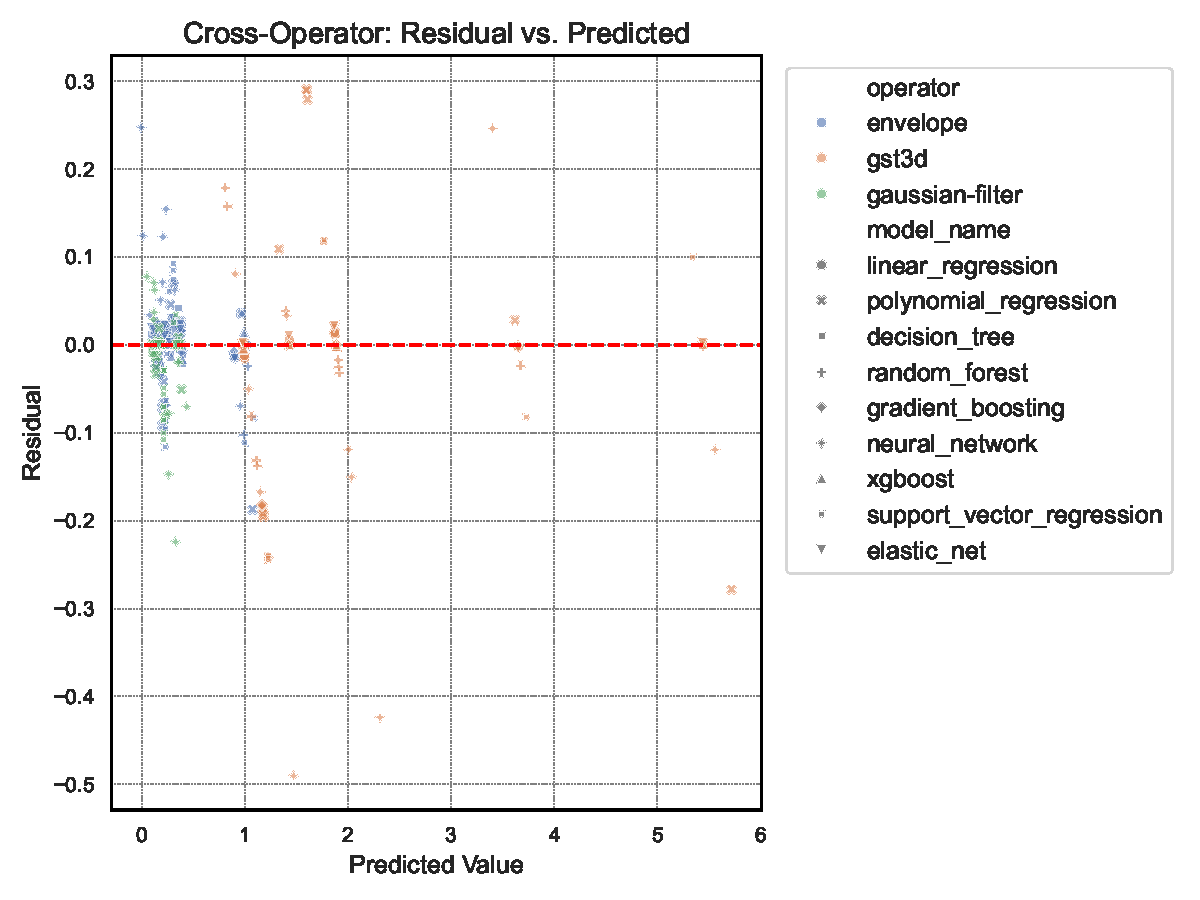
\includegraphics[width=\textwidth]{assets/images/05/residual_vs_predicted}
        \caption{Residual vs.\ predicted values for all operators and models.
            Most models yield low residuals across a wide range of predicted values.
            The \ac{GST3D}–Neural Network pairing stands out for higher errors.
            \EB{Adicione a unidade de medida nos rótulos dos eixos: p.ex.: Residual (GB?) e Predicted Value (GB?)}
        }
    \end{subfigure}
    \hfill
    \begin{subfigure}[t]{0.49\textwidth}
        \centering
        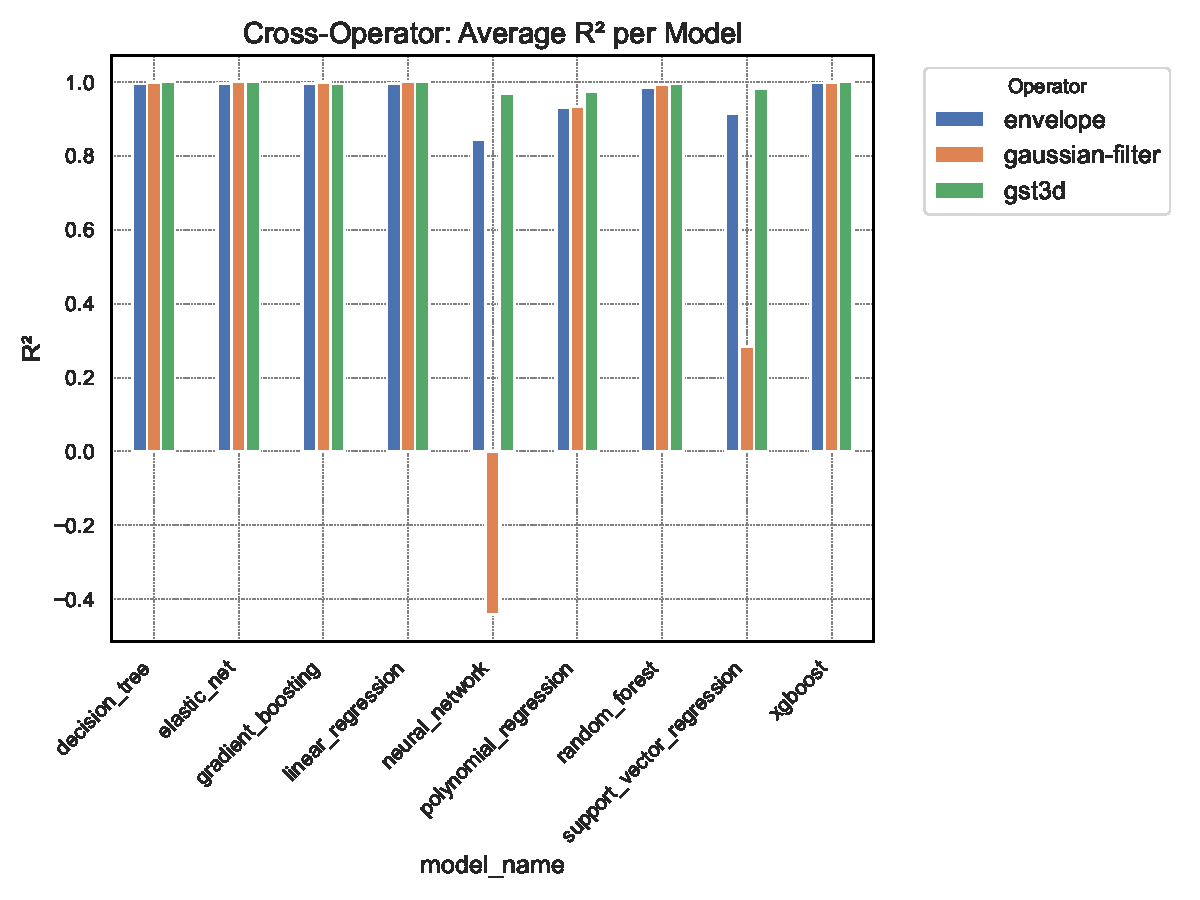
\includegraphics[width=\textwidth]{assets/images/05/cross_model_r2_bar}
        \caption{$R^2$ scores for each model and operator.
        Linear Regression, XGBoost, and Elastic Net perform consistently well.
        The Neural Network underperforms for \ac{GST3D}.}
    \end{subfigure}
    \caption{Overview of cross-model results: (a) residual-versus-predicted scatter plots and (b) $R^2$ bar chart.
        Simpler or regularized linear methods often yield the most stable fits.
        \EB{As fontes destes gráficos estão muito pequenas. Acho que ficaria melhor separar em dois gráficos. Não tenho certeza, mas talvez os dados do gráfico (b) fiquem melhor em uma tabela.}
        \label{fig:residual_vs_predicted_and_r2_bar}
    }
\end{figure*}

Table~\ref{tab:performance_summary} summarizes the main metrics for each operator, aggregated over the nine models.
These data are distilled from the experiment’s \texttt{model\_metrics.csv} files (Envelope, \ac{GST3D}, Gaussian Filter).
The best \EBC{“score”}{definir esta métrica} values for Envelope, \ac{GST3D}, and Gaussian Filter are $2.579$, $2.970$, and $2.904$, respectively.
Gradient Boosting tops Envelope, Decision Tree leads \ac{GST3D}, and Linear Regression narrowly surpasses Elastic Net for the Gaussian Filter.

\begin{table}[htbp]
    \centering
    \begin{tabular}{lccc}
        \hline
        \textbf{Operator} & \textbf{Best Model} & \textbf{Best Score} & \textbf{Note}                    \\
        \hline
        Envelope          & Gradient Boosting   & 2.579               & Consistently low RMSE            \\
        \ac{GST3D}        & Decision Tree       & 2.970               & Highest $R^2$, minimal residuals \\
        Gaussian Filter   & Linear Regression   & 2.904               & Ties closely with Elastic Net    \\
        \hline
    \end{tabular}
    \caption{Summary of top-performing models and their best “score” metric across operators.}
    \label{tab:performance_summary}
\end{table}

\subsection{Operator-Specific Model Scores}
\label{subsec:operator-specific-model-scores}

Figures~\ref{fig:score_by_model_operators} and~\ref{fig:best_model_per_operator} break down model \EBC{scores}{definir esta métrica} per operator and highlight the winning algorithm in each category.
The minor differences among the leading models (Gradient Boosting, XGBoost, Decision Tree, and Linear/Elastic Net) suggest that seismic memory usage is comparatively straightforward to learn, likely due to the near-linear volume relationship observed in Section~\ref{sec:pmc-results-memory-and-execution-time-profiling}.

\begin{figure*}[htbp]
    \centering
    \begin{subfigure}[t]{0.32\textwidth}
        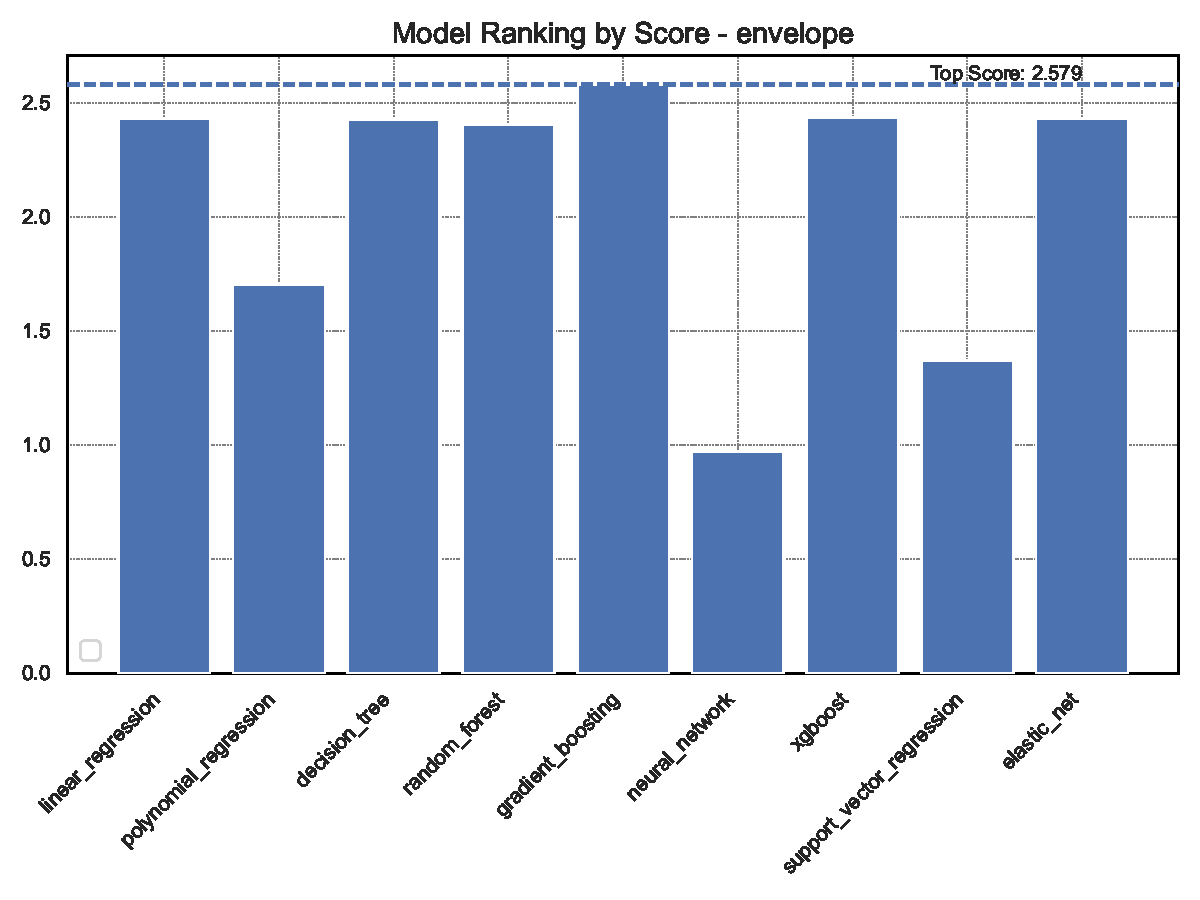
\includegraphics[width=\textwidth]{assets/images/05/score_by_model_envelope}
        \caption{Envelope}
    \end{subfigure}
    \hfill
    \begin{subfigure}[t]{0.32\textwidth}
        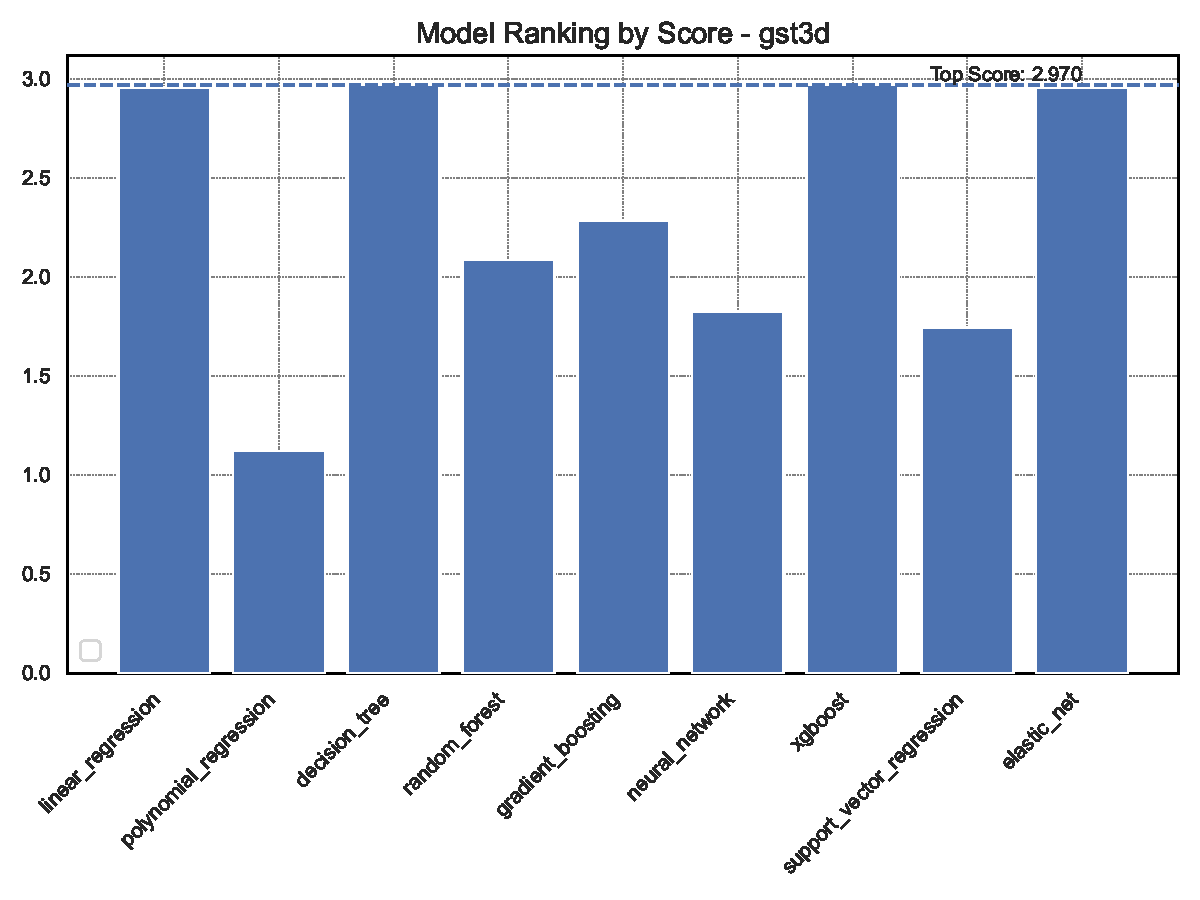
\includegraphics[width=\textwidth]{assets/images/05/score_by_model_gst3d}
        \caption{\ac{GST3D}}
    \end{subfigure}
    \hfill
    \begin{subfigure}[t]{0.32\textwidth}
        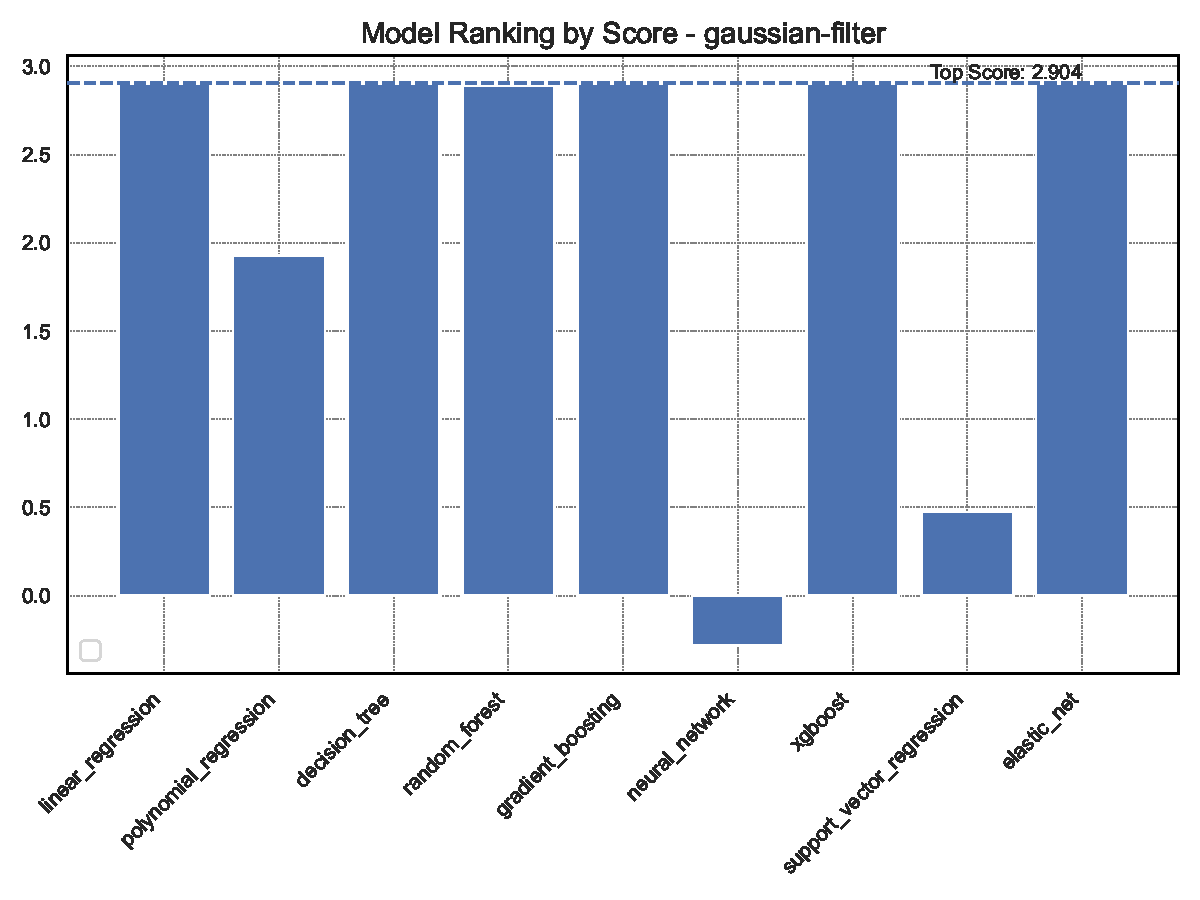
\includegraphics[width=\textwidth]{assets/images/05/score_by_model_gaussian-filter}
        \caption{Gaussian Filter}
    \end{subfigure}
    \caption{\EBC{Scores by model for each operator}{definir a métrica score}.
        A higher score indicates stronger overall performance.
        Multiple models cluster near the top for all three operators, highlighting the relative ease of predicting memory usage from linear shape parameters.
        \label{fig:score_by_model_operators}
    }
\end{figure*}

\begin{figure}[htbp]
    \centering
    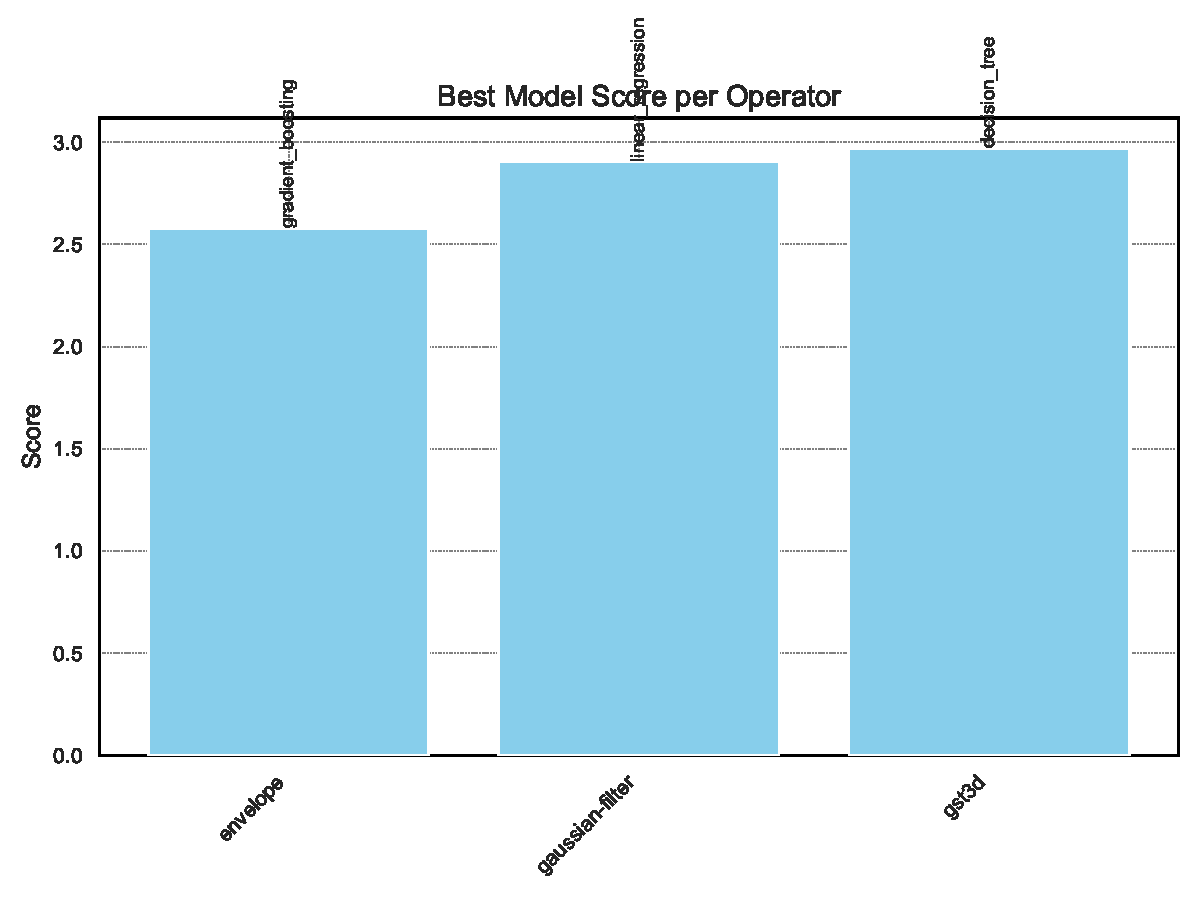
\includegraphics[width=0.6\textwidth]{assets/images/05/best_model_per_operator}
    \caption{Best model per operator by score: Gradient Boosting (Envelope), Decision Tree (\ac{GST3D}), and Linear Regression (Gaussian Filter).
        \EB{Senti falta da definição da métrica "Score"}
        \label{fig:best_model_per_operator}
    }
\end{figure}

\subsection{Accuracy and RMSE Analysis}
\label{subsec:accuracy-and-rmse-analysis}

\EBC{Como você definiu/calculou acurácia?}

Figure~\ref{fig:accuracy_rmse_envelope} illustrates accuracy versus \ac{RMSE} for each model under Envelope, \ac{GST3D}, and Gaussian Filter.
An ideal model would appear near the top-left corner (high accuracy, low \ac{RMSE}).
Polynomial Regression and the Neural Network exhibit relatively higher \ac{RMSE} in \ac{GST3D}, reinforcing the patterns already noted in the residual plots and $R^2$ bars.

\begin{figure*}[htbp]
    \centering
    \begin{subfigure}[t]{0.32\textwidth}
        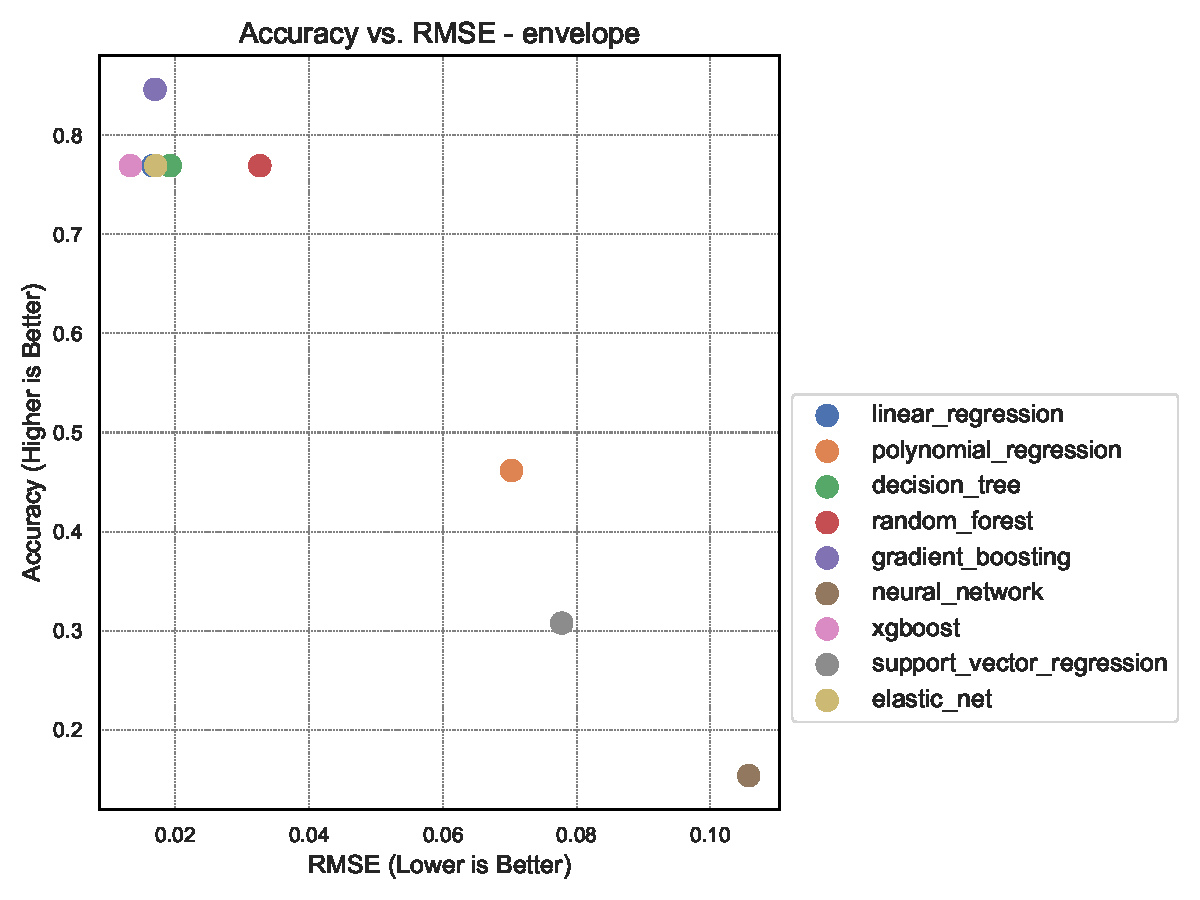
\includegraphics[width=\textwidth]{assets/images/05/accuracy_by_rmse_per_model_envelope}
        \caption{Envelope}
    \end{subfigure}
    \hfill
    \begin{subfigure}[t]{0.32\textwidth}
        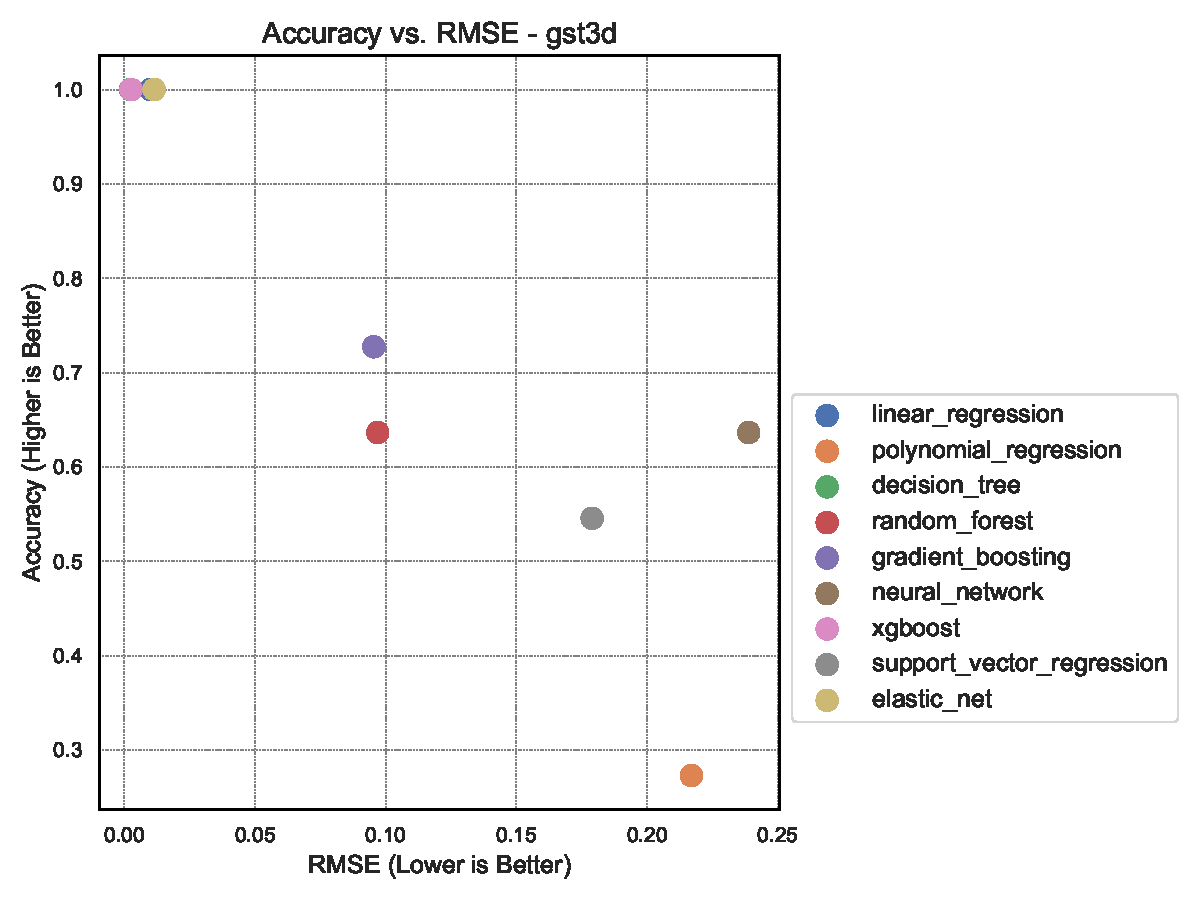
\includegraphics[width=\textwidth]{assets/images/05/accuracy_by_rmse_per_model_gst3d}
        \caption{\ac{GST3D}}
    \end{subfigure}
    \hfill
    \begin{subfigure}[t]{0.32\textwidth}
        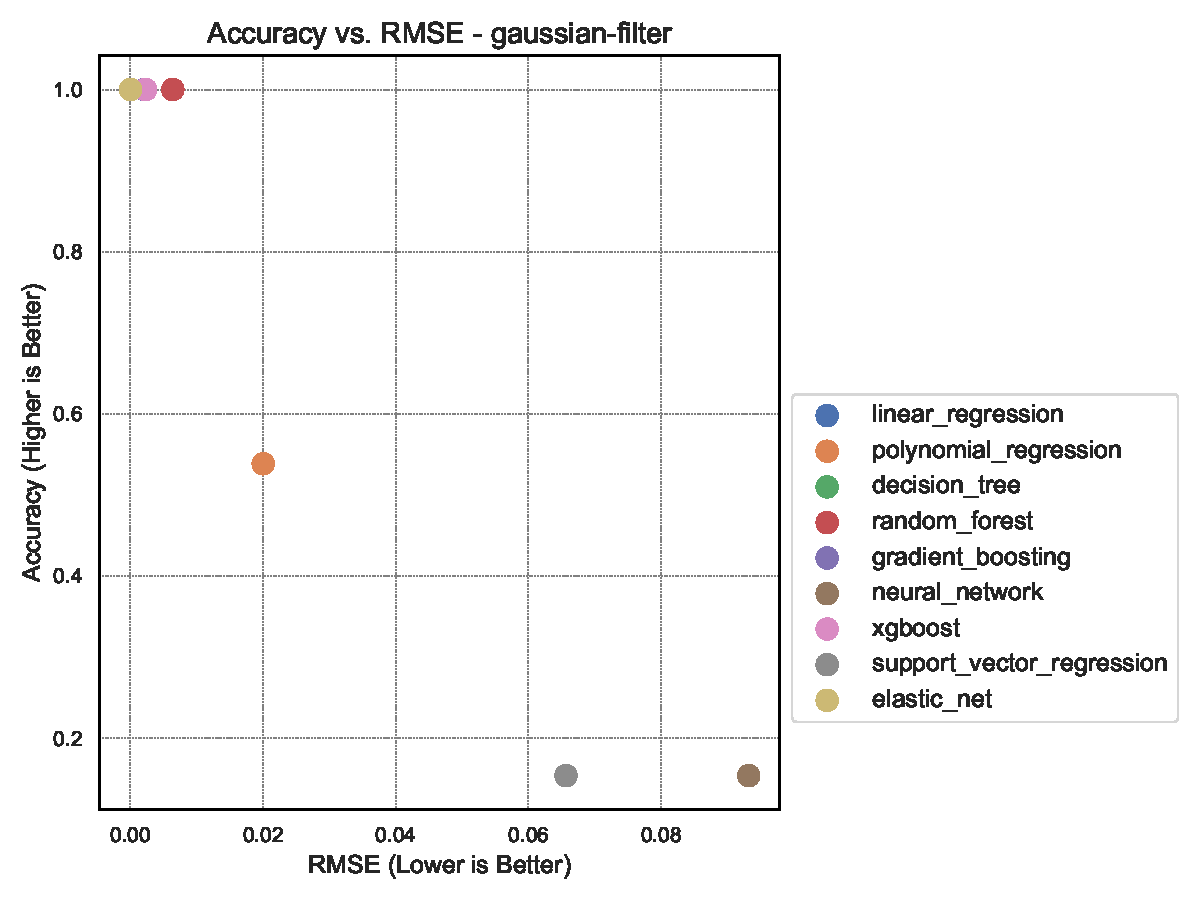
\includegraphics[width=\textwidth]{assets/images/05/accuracy_by_rmse_per_model_gaussian-filter}
        \caption{Gaussian Filter}
    \end{subfigure}
    \caption{Accuracy vs.\ \ac{RMSE} per model and operator.
        Most methods attain near-perfect metrics for Envelope and Gaussian Filter.
        \ac{GST3D} displays higher \ac{RMSE} for polynomial and Neural Network approaches.
        \EB{Acho que ficaria melhor compartilhando a legenda - com apenas uma legenda.}
    }
    \label{fig:accuracy_rmse_envelope}
\end{figure*}

\subsection{Actual vs.\ Predicted Plots and Residual Distributions}
\label{subsec:actual-vs-predicted-and-residual-distributions}

Figure~\ref{fig:actual_vs_predicted} compare actual and predicted memory usage for each operator and model.
The best fits produce data points that lie close to the diagonal line, implying minimal error.
Linear Regression, XGBoost, and Elastic Net nearly overlap with the diagonal for Envelope and Gaussian Filter.
Decision Tree does likewise for \ac{GST3D}.

\begin{figure*}[htbp]
    \centering
    \begin{subfigure}[t]{0.32\textwidth}
        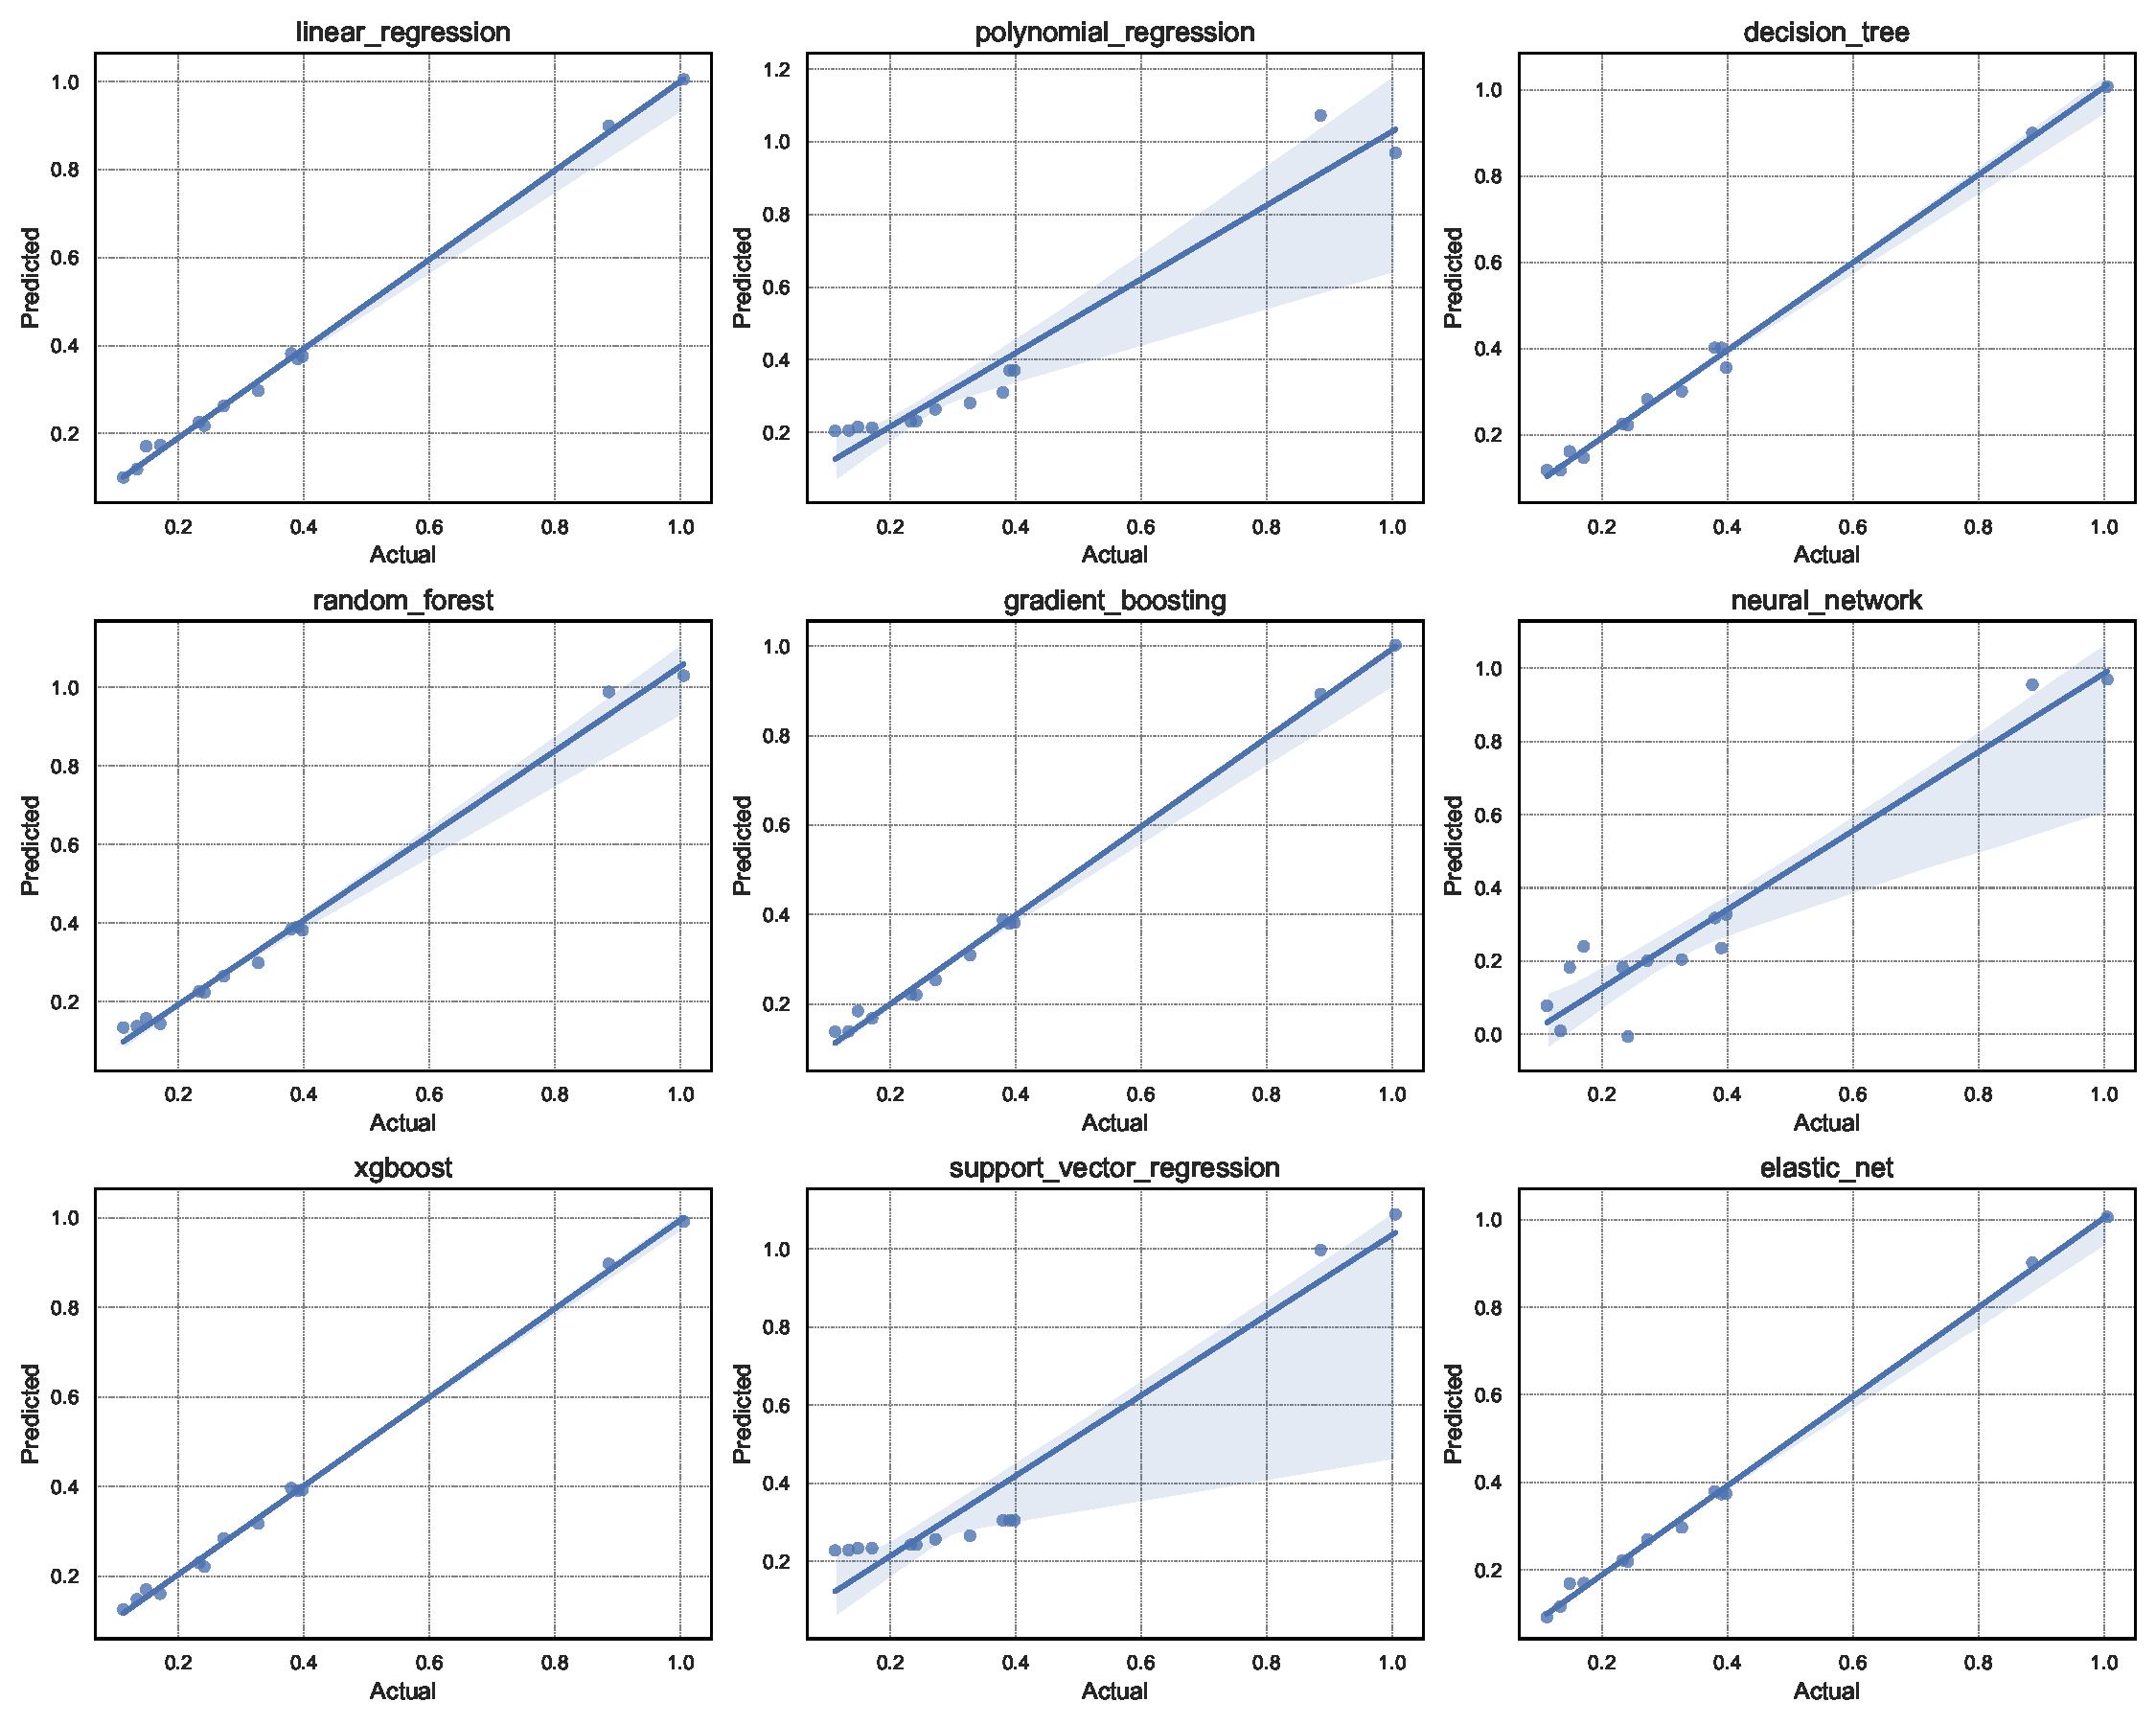
\includegraphics[width=\textwidth]{assets/images/05/actual_vs_predicted_by_model_envelope}
        \caption{Envelope}
    \end{subfigure}
    \hfill
    \begin{subfigure}[t]{0.32\textwidth}
        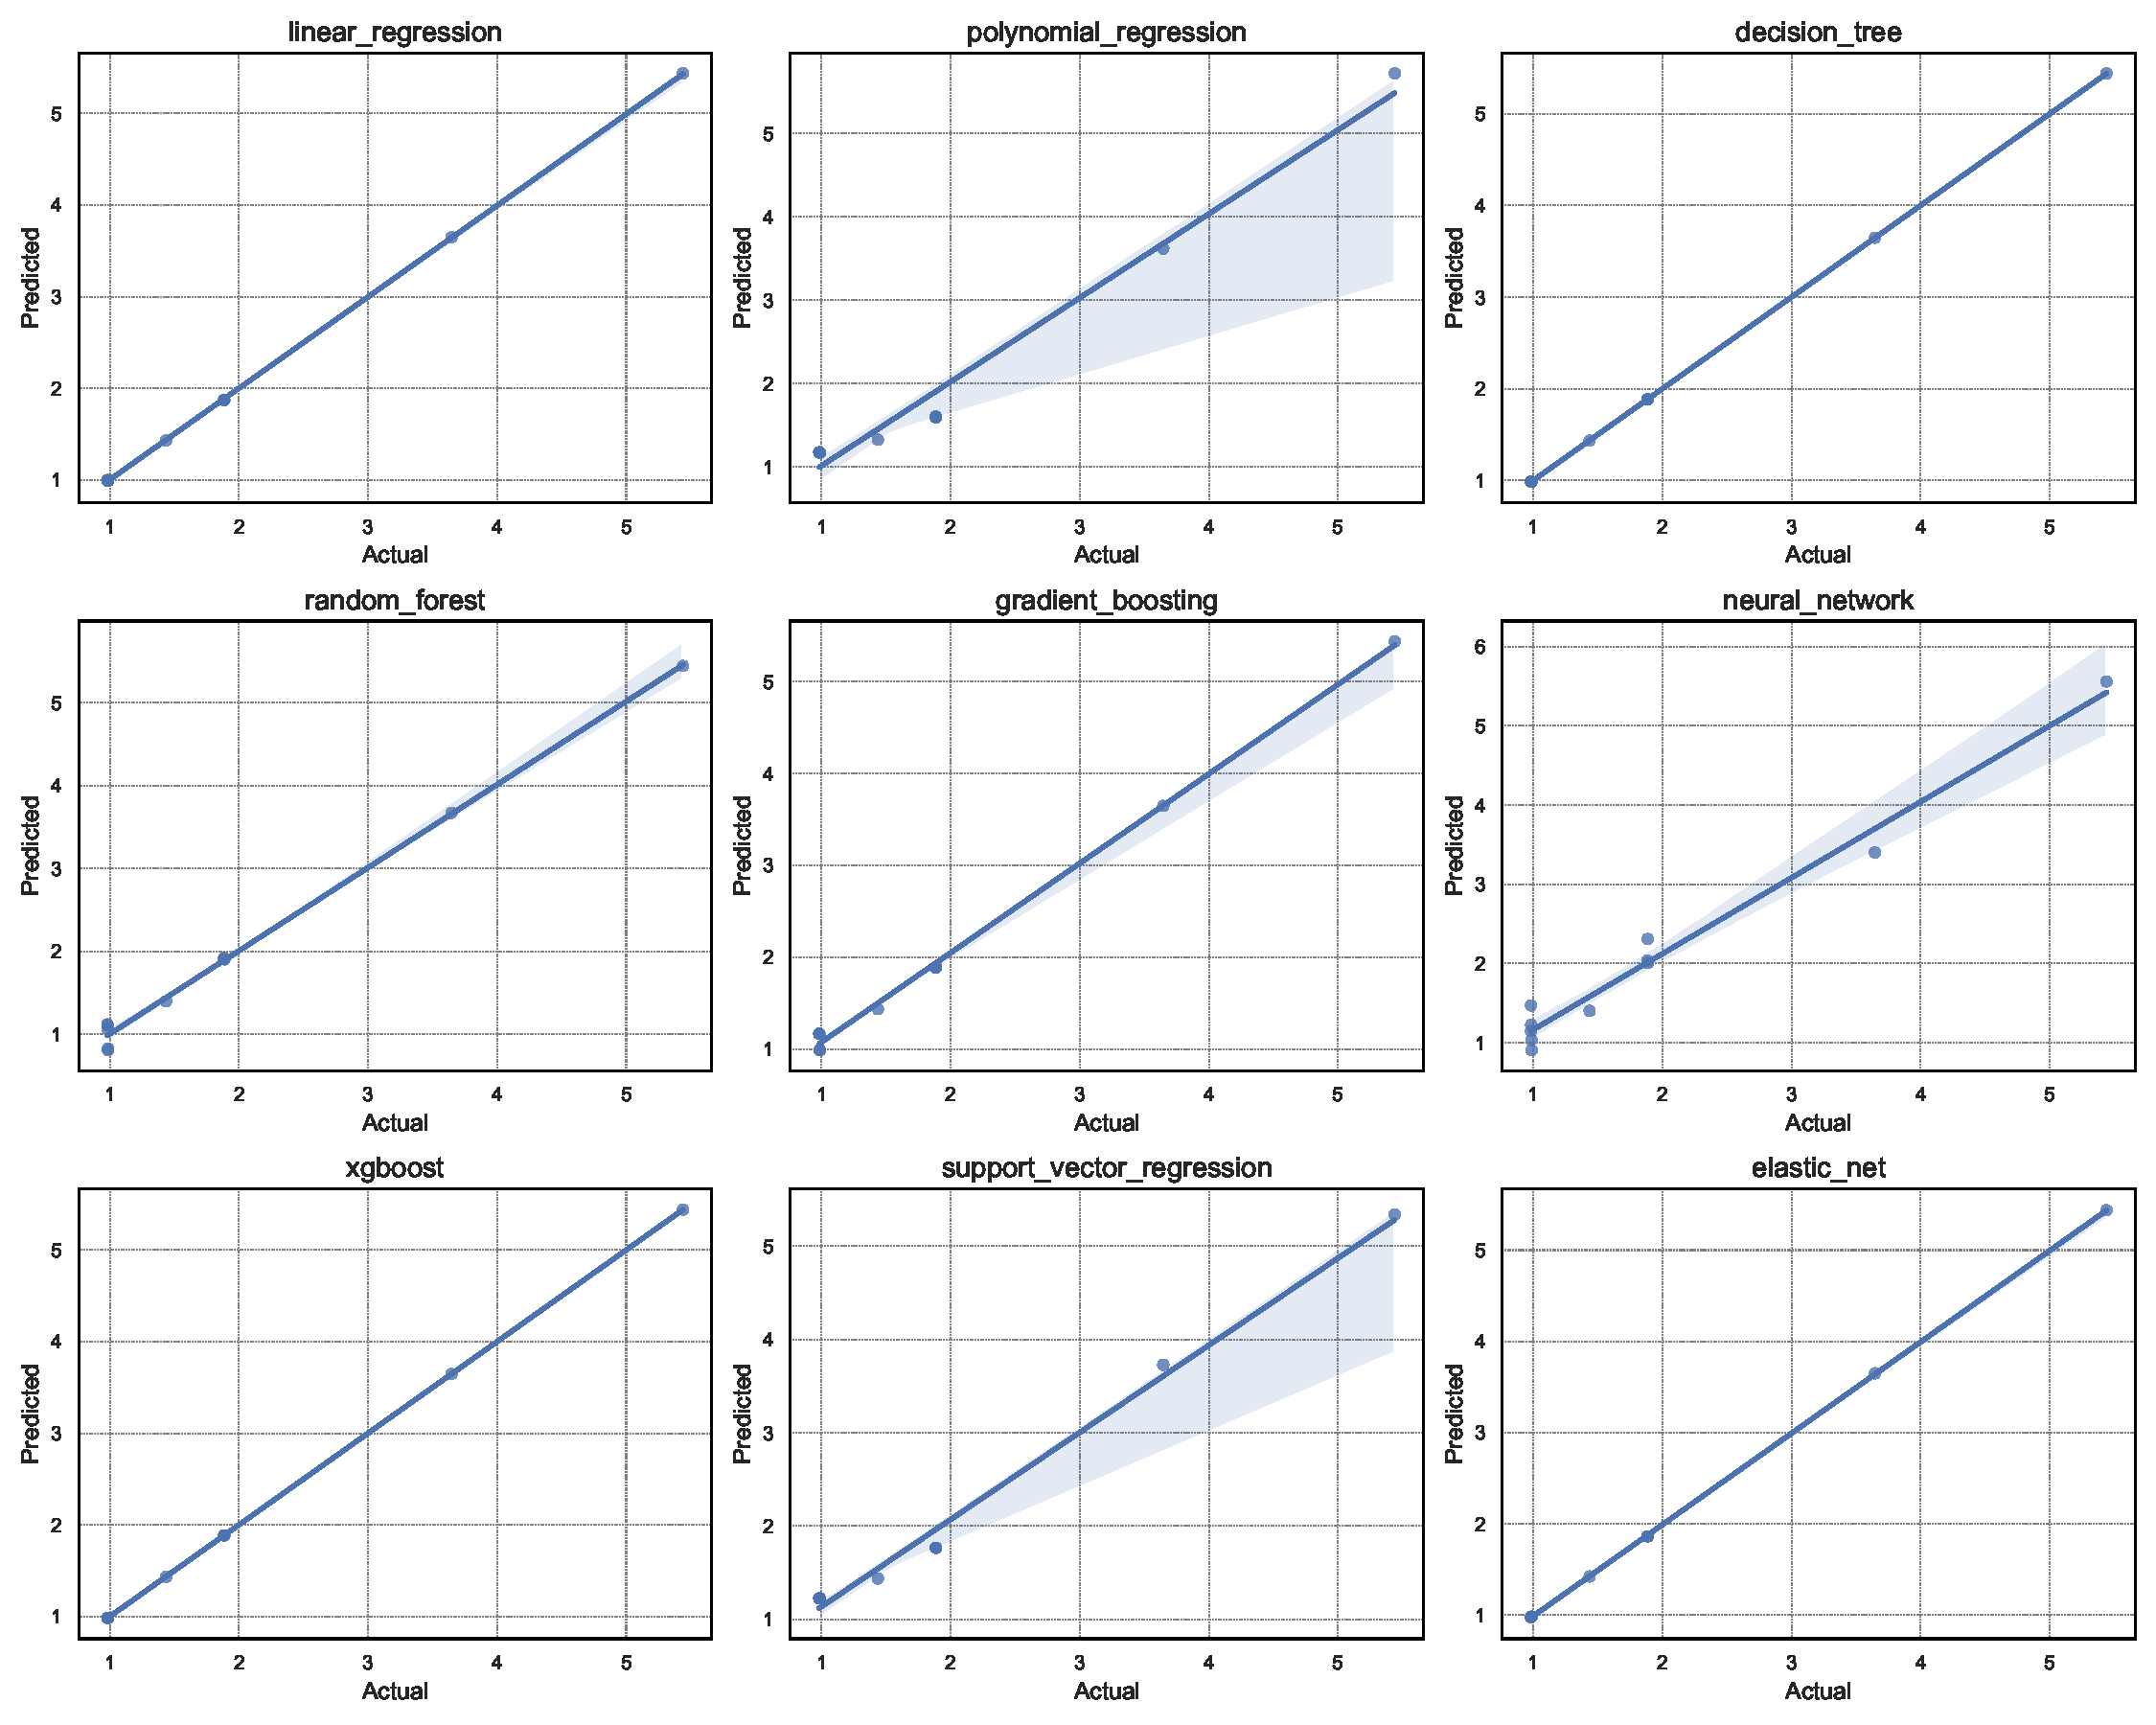
\includegraphics[width=\textwidth]{assets/images/05/actual_vs_predicted_by_model_gst3d}
        \caption{\ac{GST3D}}
    \end{subfigure}
    \hfill
    \begin{subfigure}[t]{0.32\textwidth}
        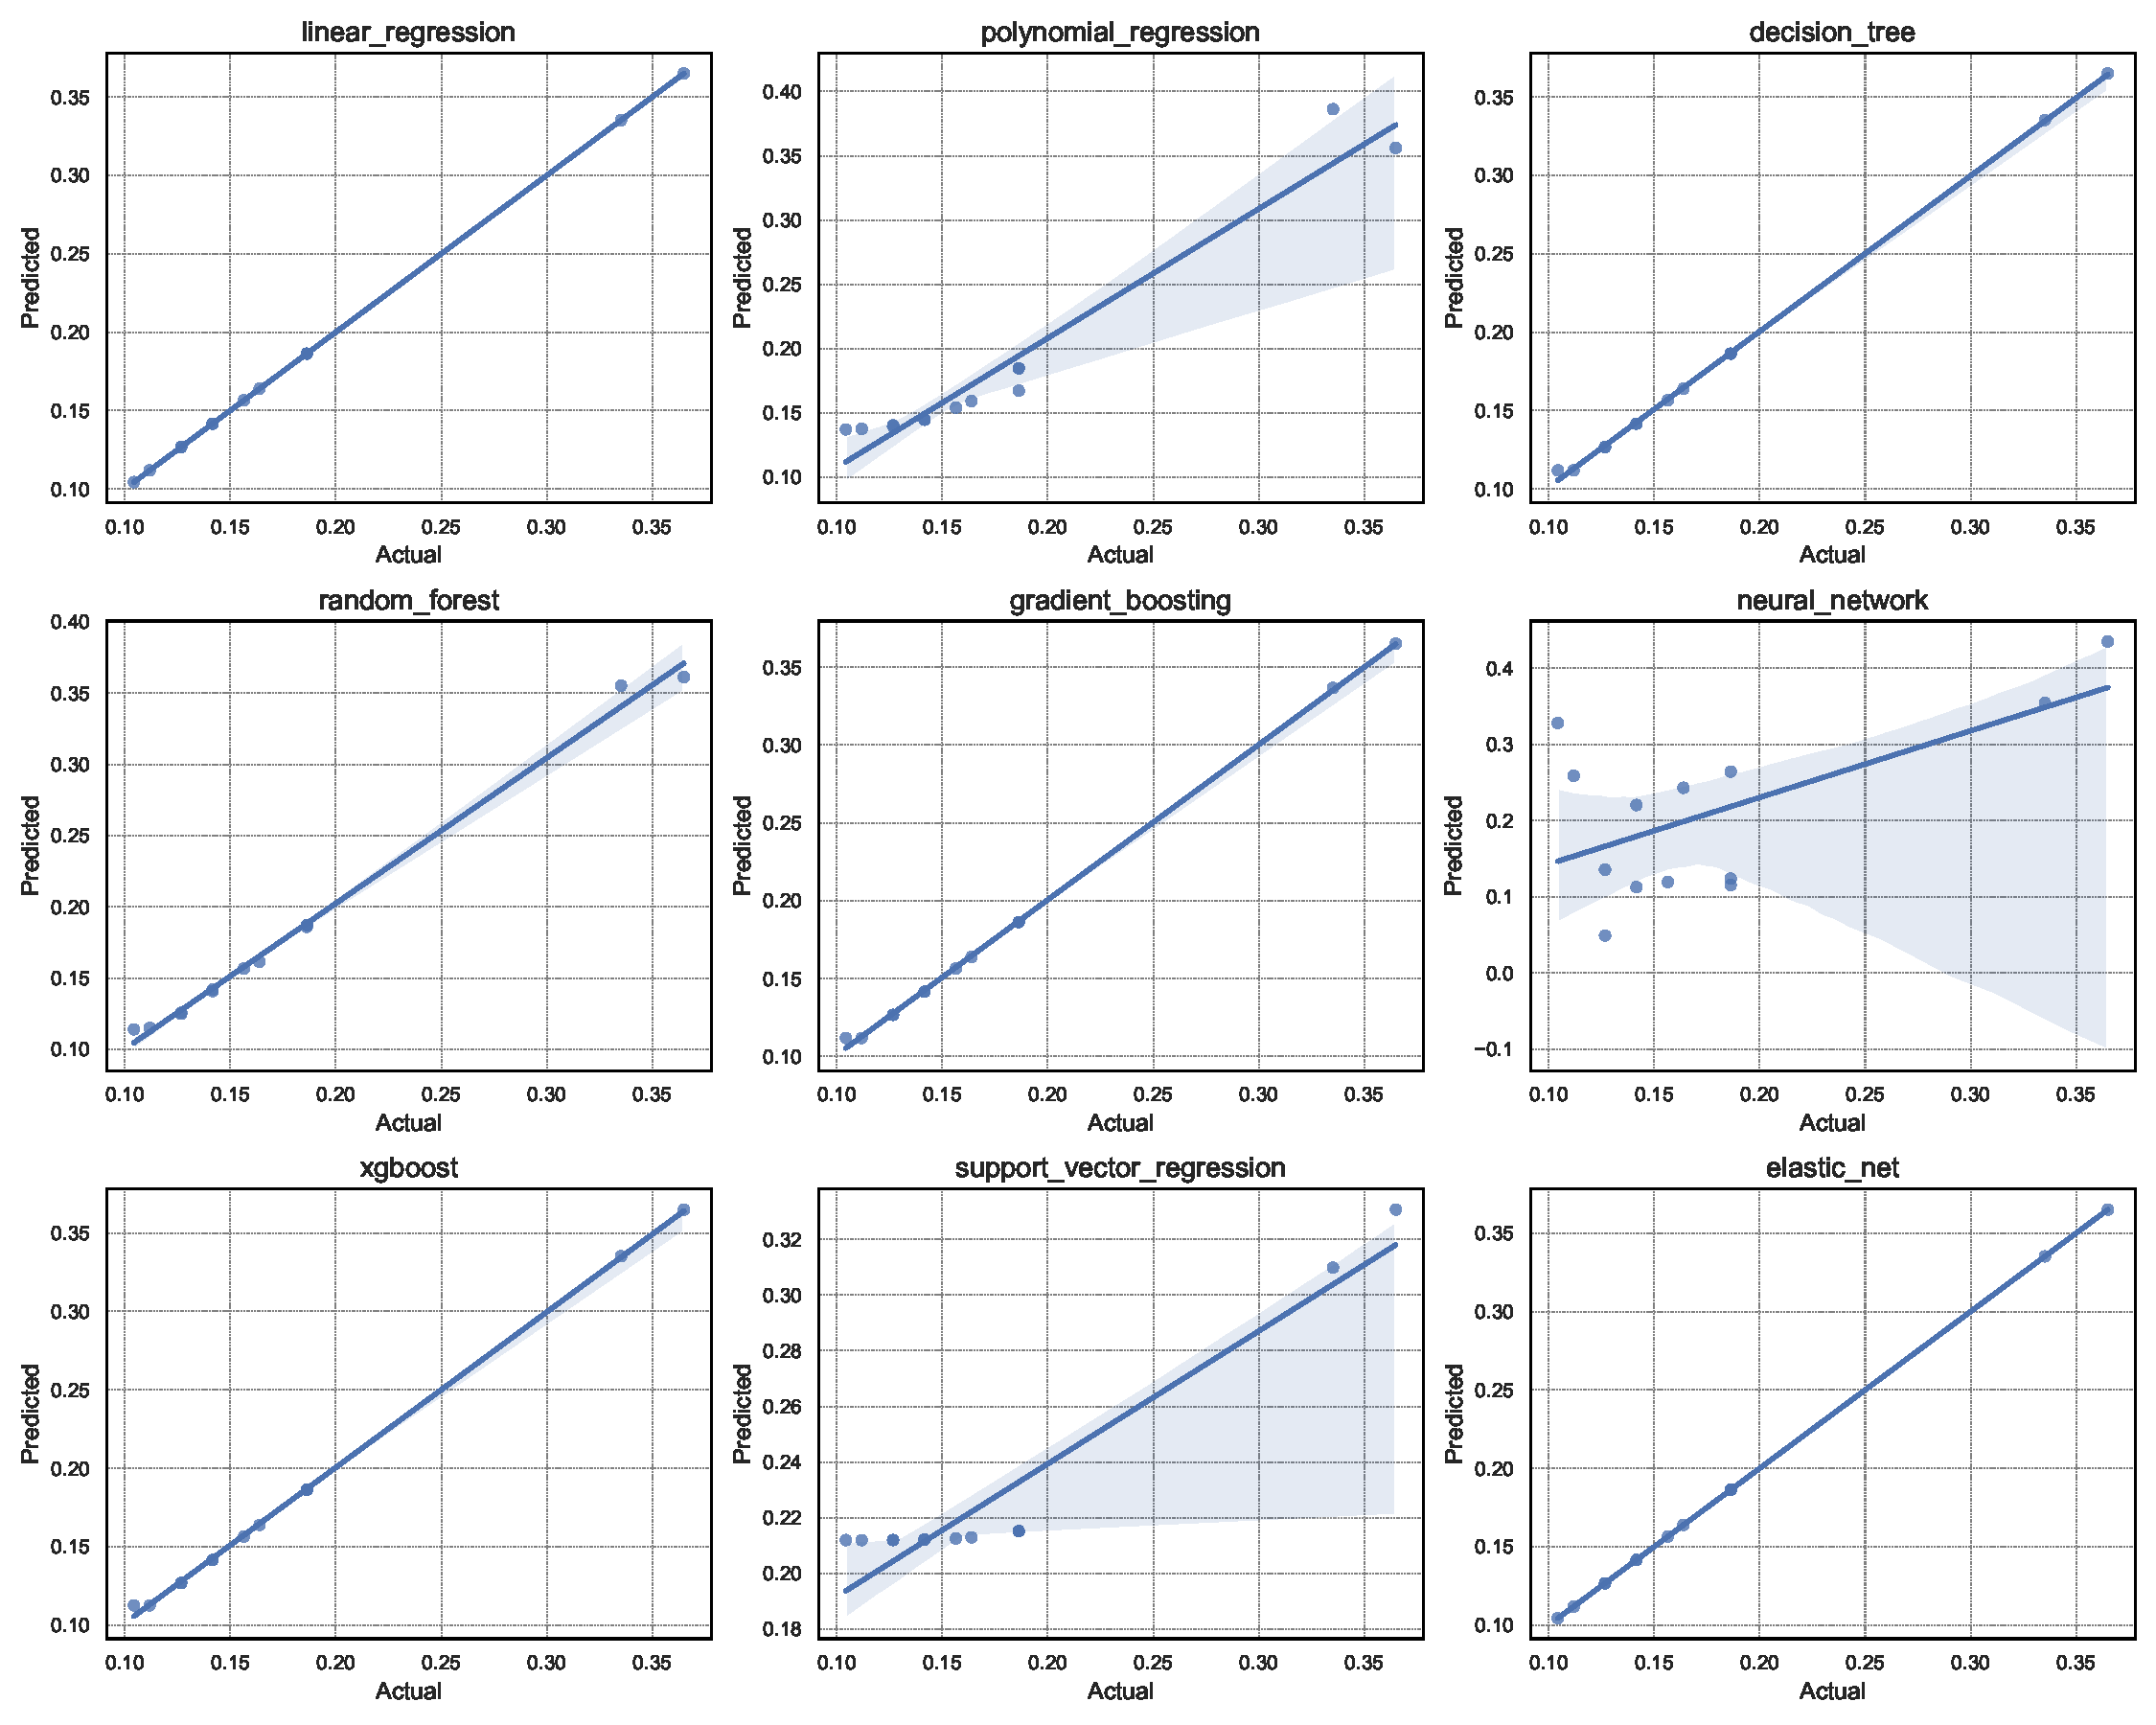
\includegraphics[width=\textwidth]{assets/images/05/actual_vs_predicted_by_model_gaussian-filter}
        \caption{Gaussian Filter}
    \end{subfigure}
    \caption{Actual vs.\ predicted memory usage for each operator.
    A nearly diagonal trend indicates that the model approximates the real consumption.
    The Neural Network struggles slightly more for \ac{GST3D}, but most others fit well.}
    \label{fig:actual_vs_predicted}
\end{figure*}

Figures~\ref{fig:residual_qq_plots} show residual \ac{QQ} plots.
Points that track the diagonal suggest normally distributed residuals, indicating no major systematic bias.
Gradient Boosting, Random Forest, and XGBoost residuals remain closer to this line than Neural Network or Polynomial Regression, which exhibit heavier tails or skew.
However, none of the models produce perfectly normal residuals, which is common in real-world \ac{HPC} \EBC{data.}{Adicionar uma referência para dar suporte a esta afirmação}

\begin{figure*}[htbp]
    \centering
    \begin{subfigure}[t]{0.32\textwidth}
        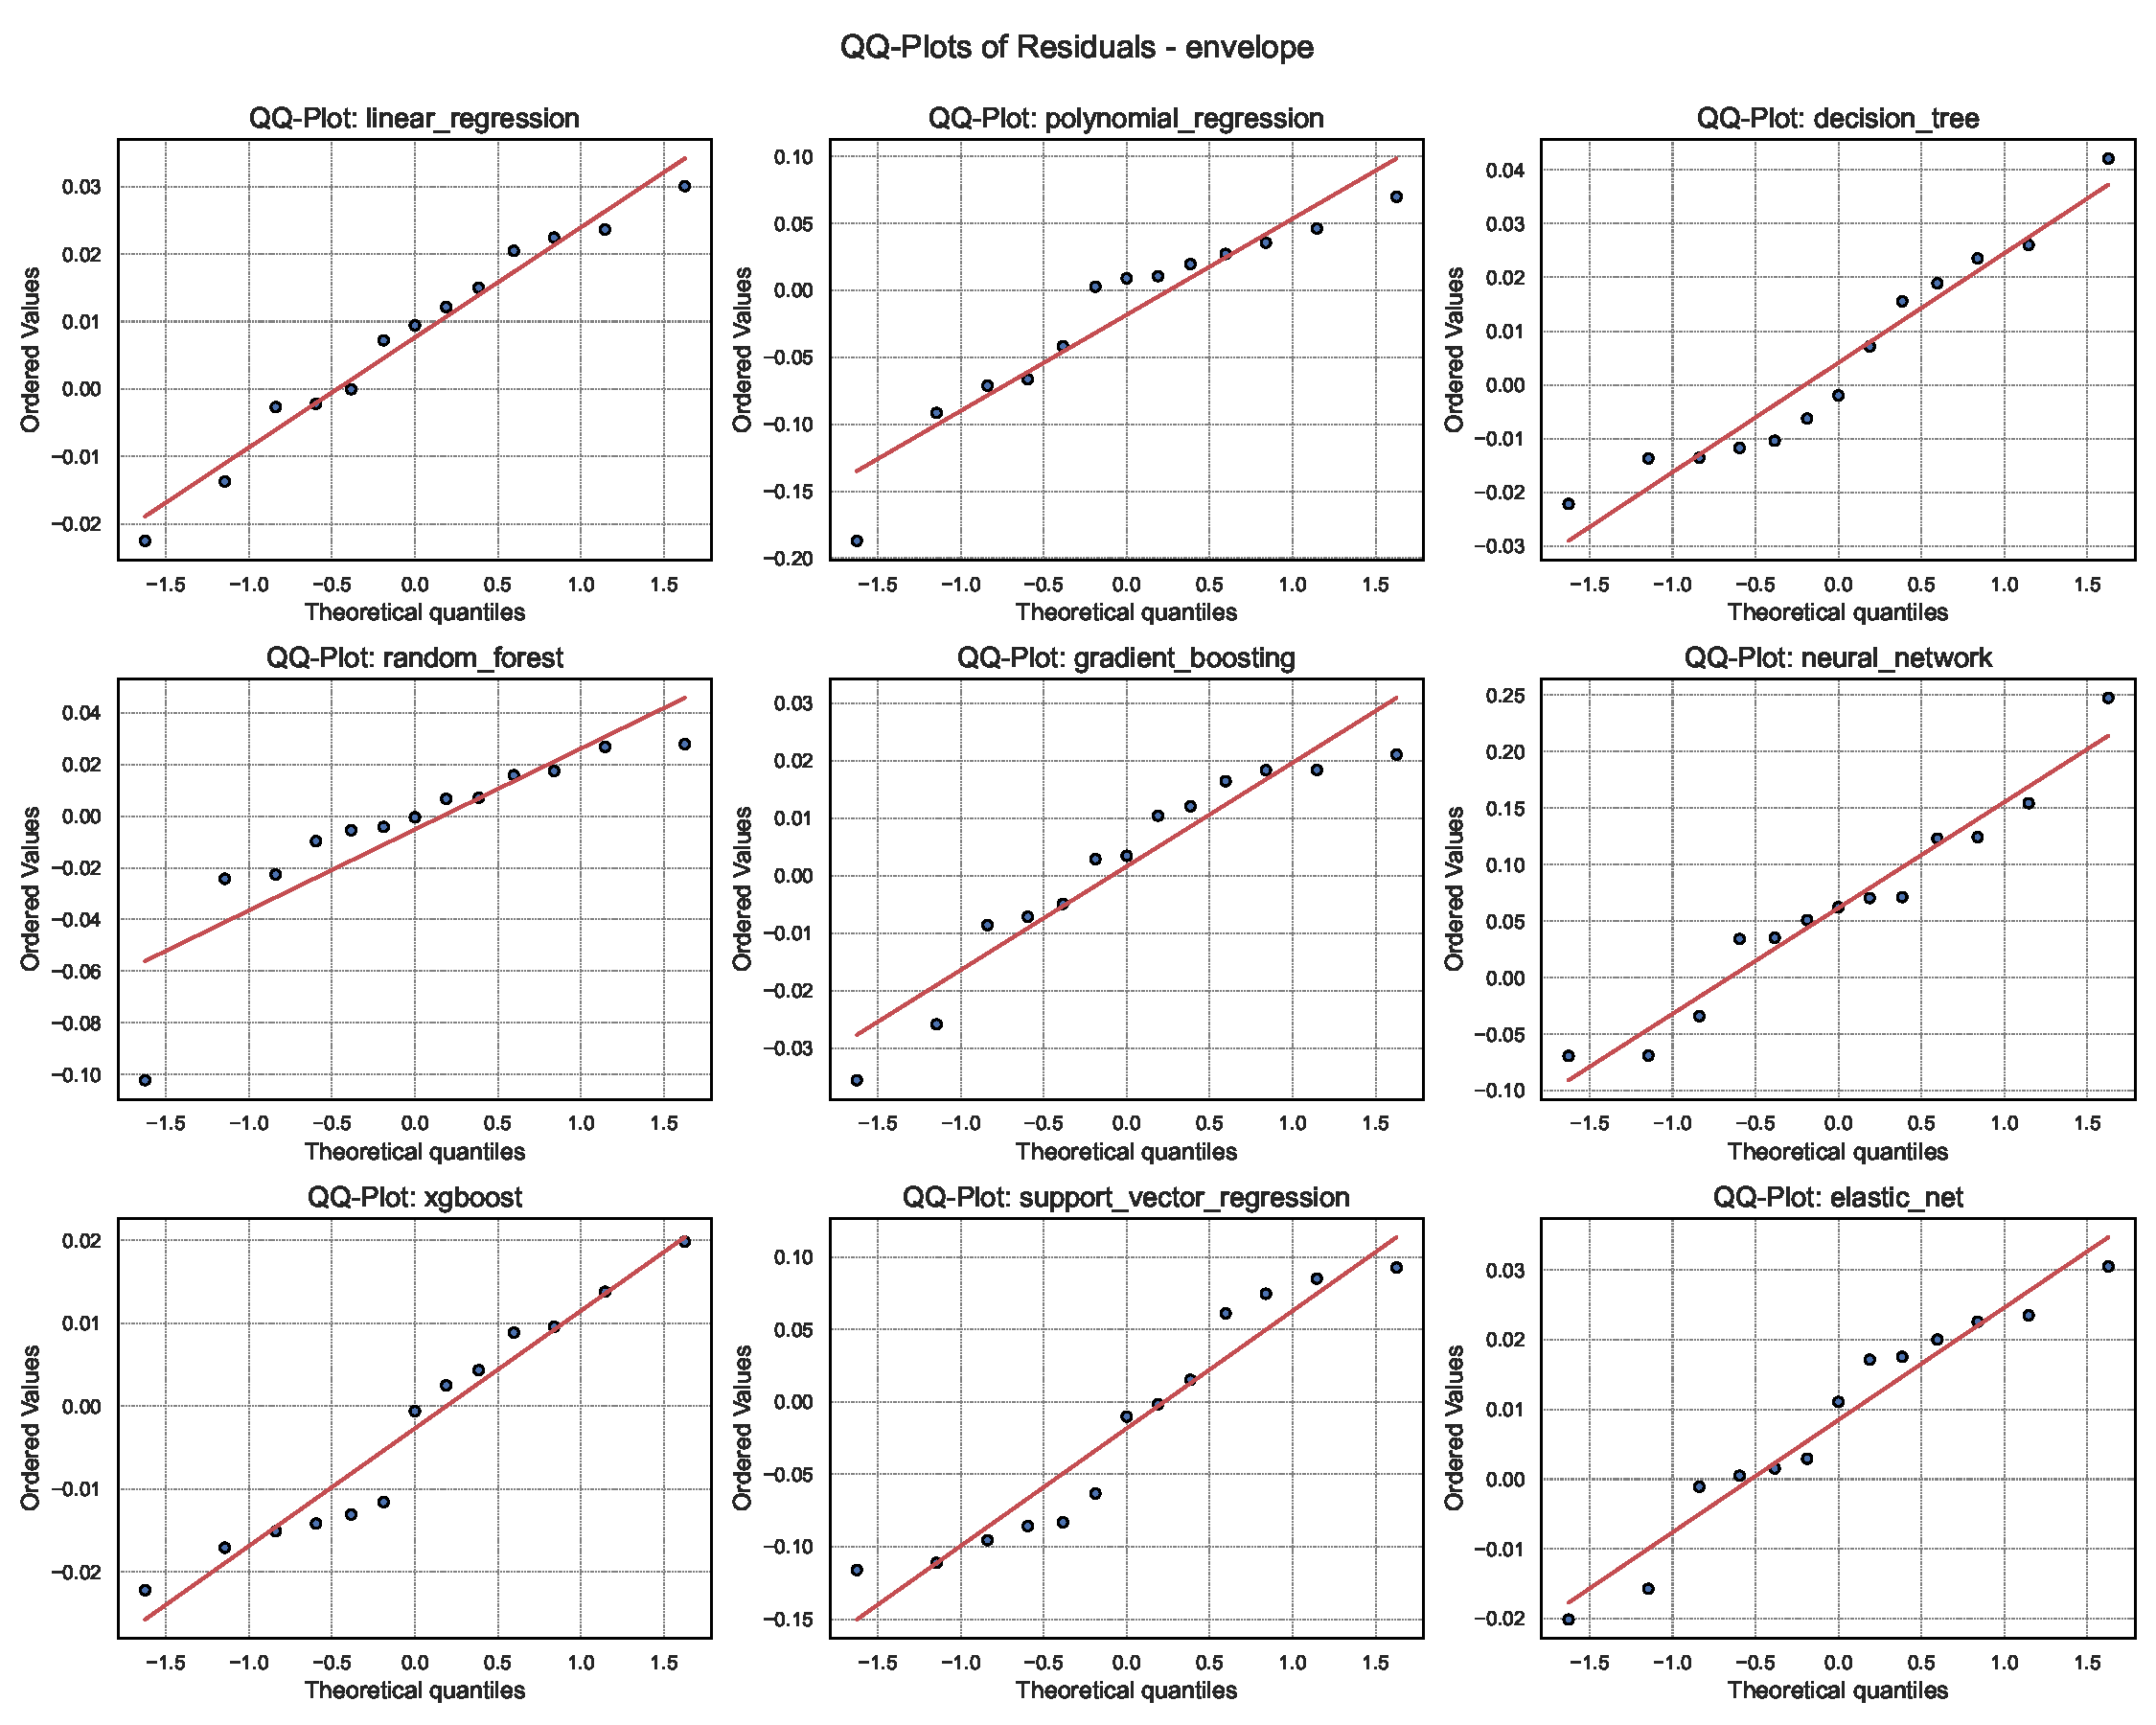
\includegraphics[width=\textwidth]{assets/images/05/residual_qq_plots_envelope}
        \caption{Envelope}
    \end{subfigure}
    \hfill
    \begin{subfigure}[t]{0.32\textwidth}
        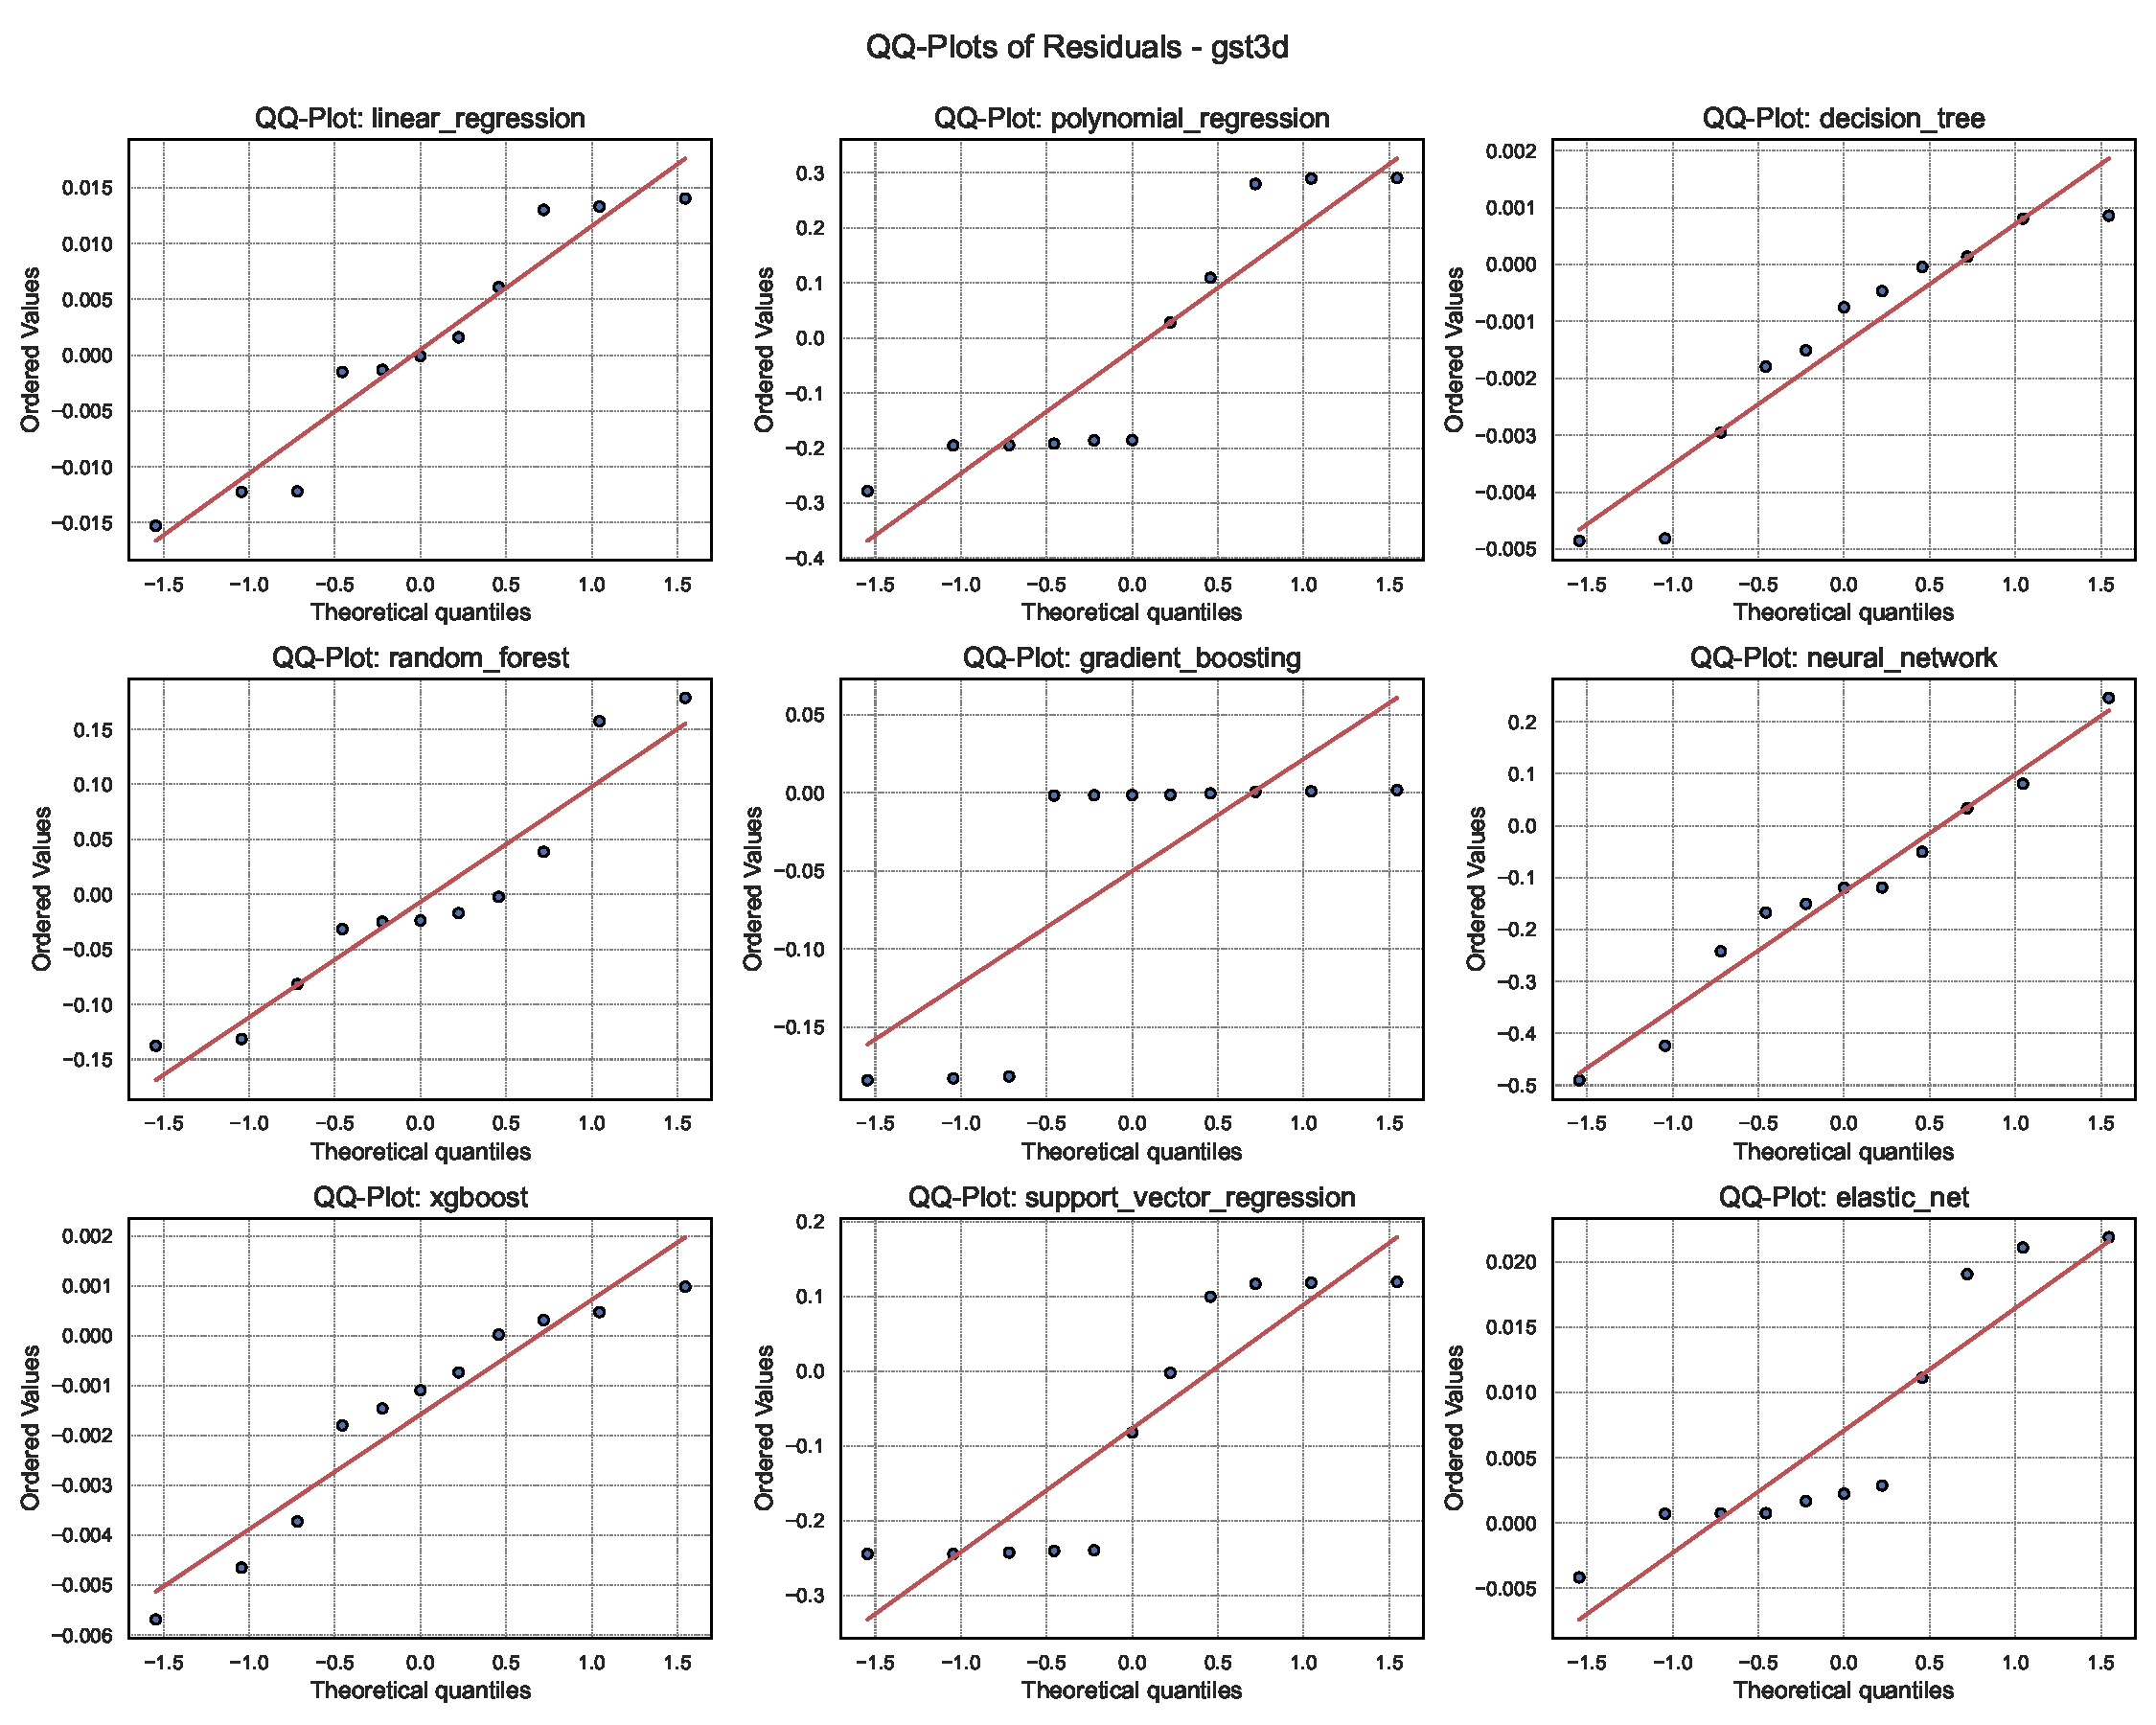
\includegraphics[width=\textwidth]{assets/images/05/residual_qq_plots_gst3d}
        \caption{\ac{GST3D}}
    \end{subfigure}
    \hfill
    \begin{subfigure}[t]{0.32\textwidth}
        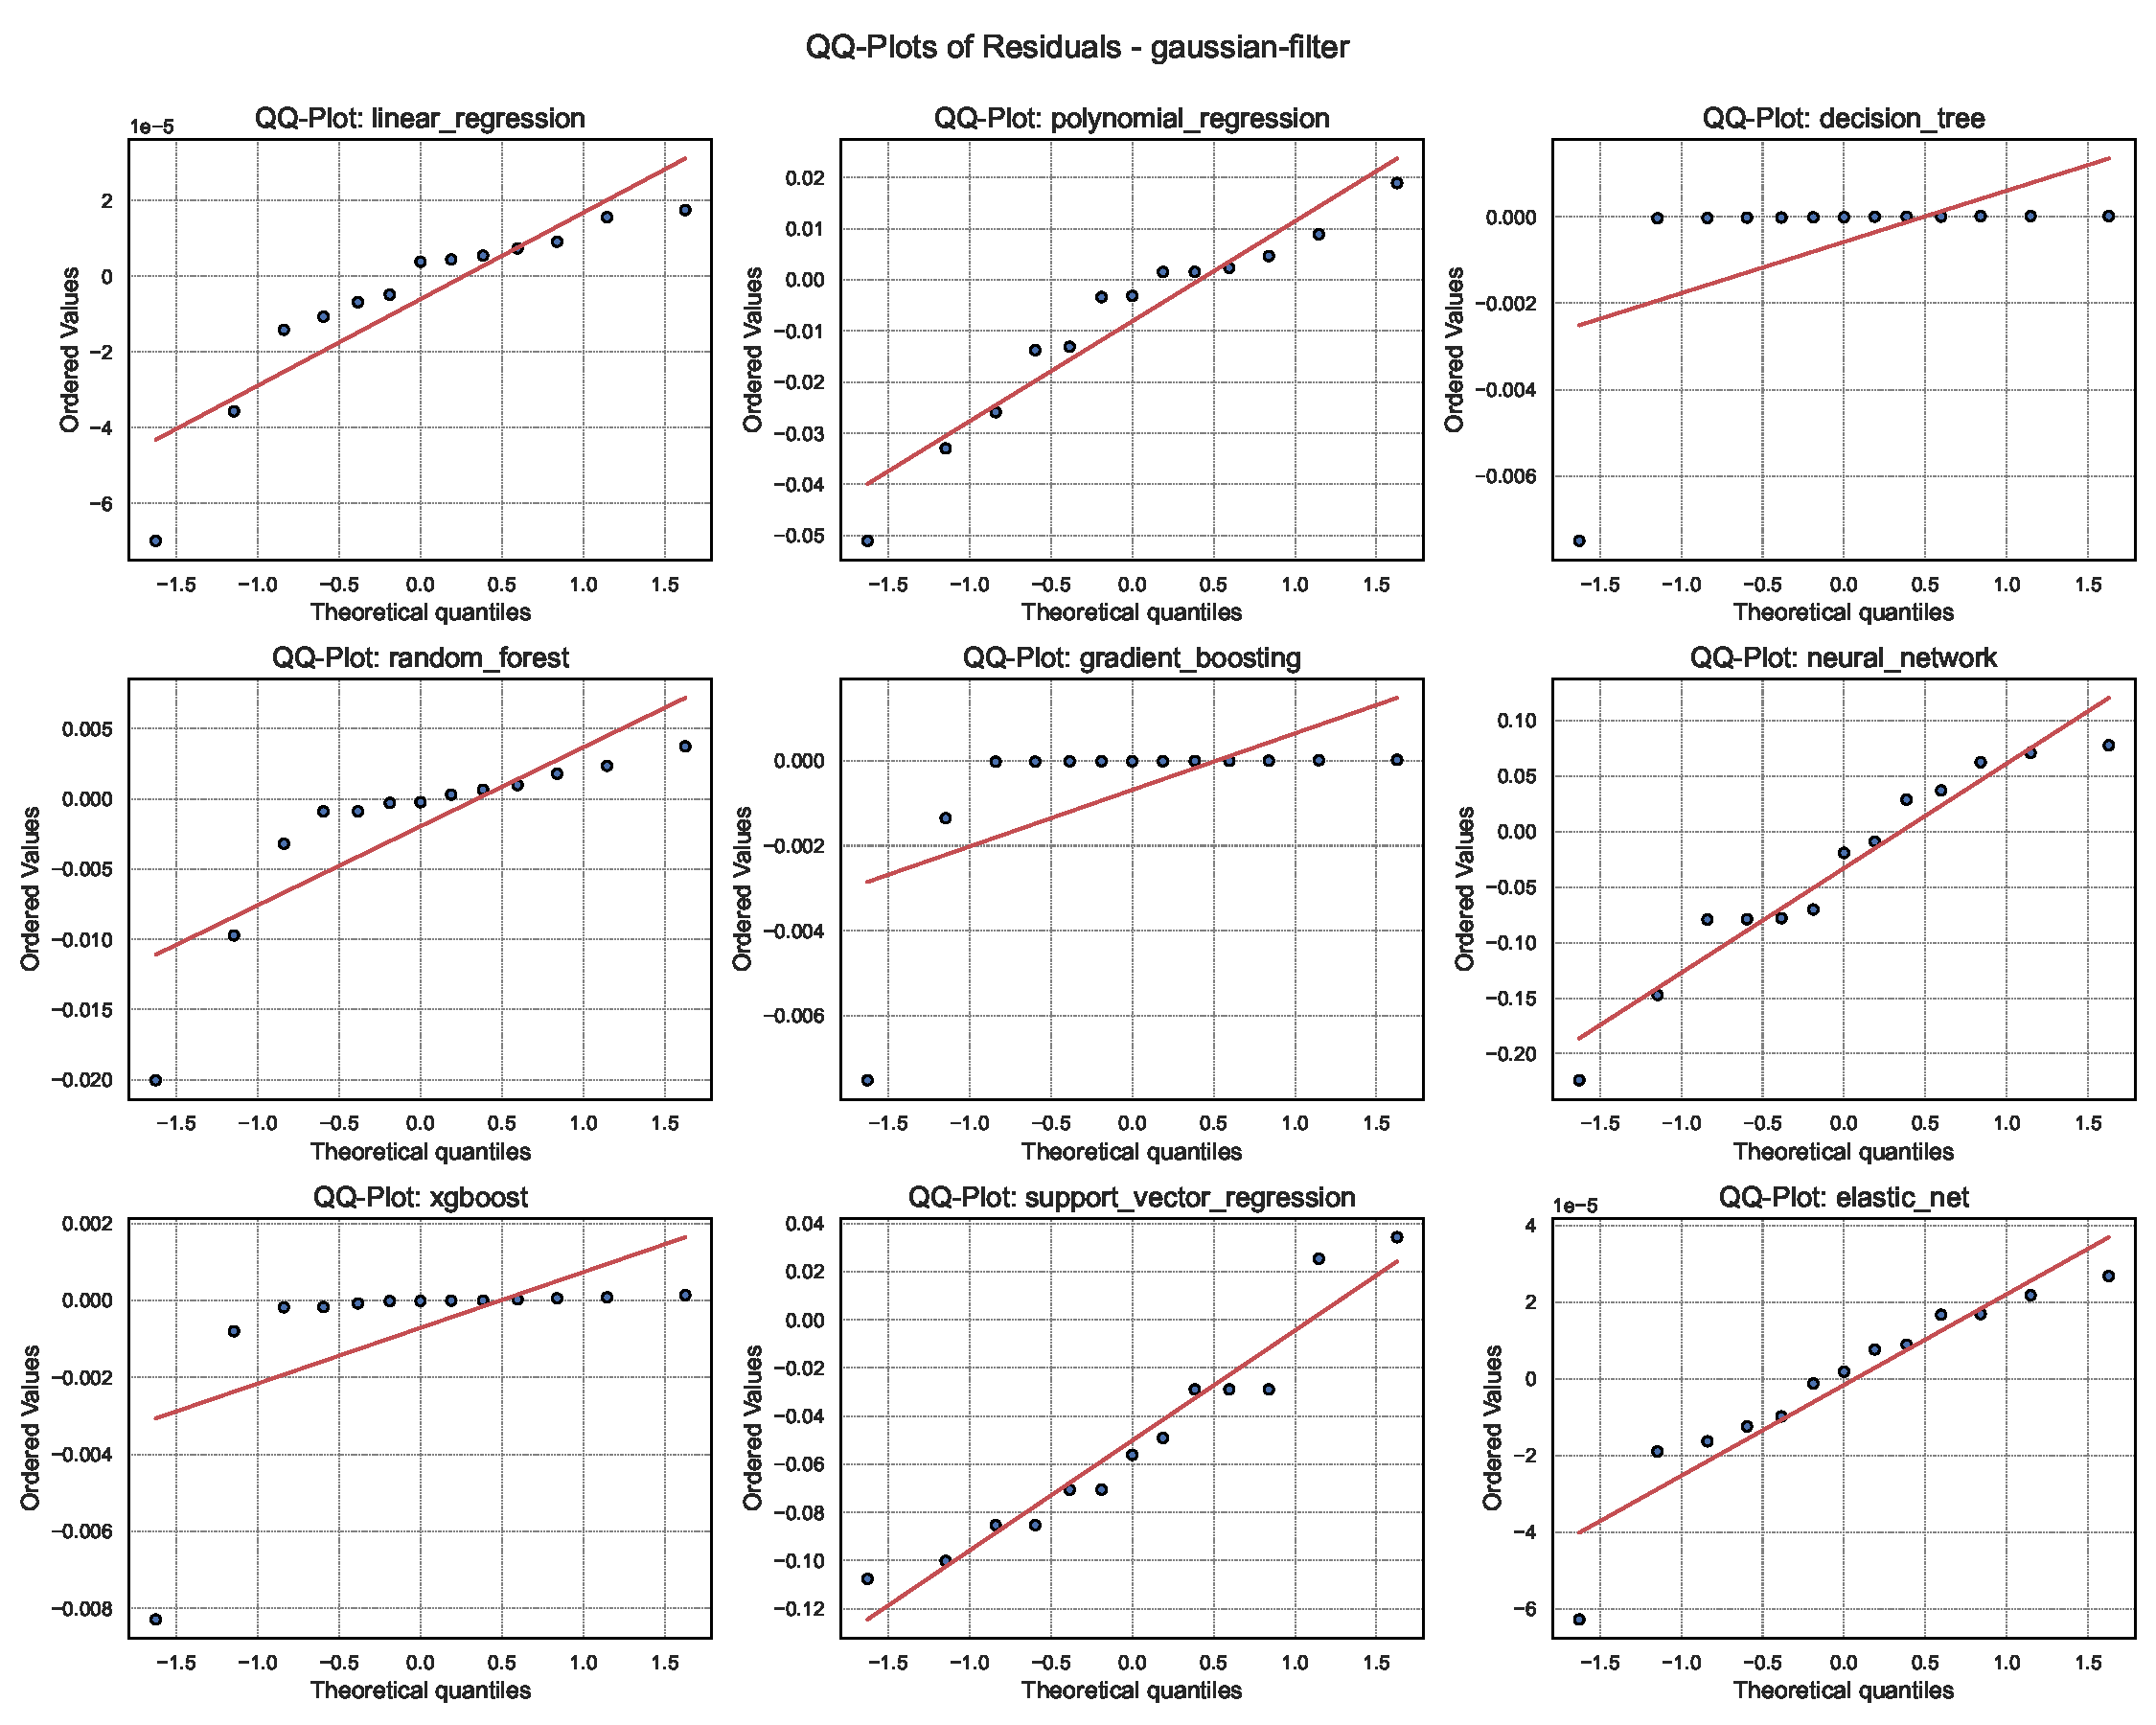
\includegraphics[width=\textwidth]{assets/images/05/residual_qq_plots_gaussian-filter}
        \caption{Gaussian Filter}
    \end{subfigure}
    \caption{\ac{QQ} plots of model residuals by operator.
        Most methods exhibit mild deviations from normality in the tails.
        Neural Network displays noticeably heavier upper-tail errors for \ac{GST3D}.
        \EB{Os rótulos ficaram muito pequenos. Será que este gráfico é necessário?}
        \label{fig:residual_qq_plots}
    }
\end{figure*}

\subsection{Performance Summary}
\label{subsec:performance-summary}

Figures~\ref{fig:performance_by_model_operators} compile \ac{RMSE}, \ac{MAE}, $R^2$, and accuracy into a single bar chart for each operator, offering a side-by-side visualization of model performance.
All charts reinforce the earlier observation that memory usage for Envelope and Gaussian Filter proves easier to capture accurately than \ac{GST3D}.
Decision Tree, Gradient Boosting, and XGBoost often yield high precision for \ac{GST3D}, whereas Neural Network and Polynomial Regression struggle with larger errors.

\begin{figure*}[htbp]
    \centering
    \begin{subfigure}[t]{0.32\textwidth}
        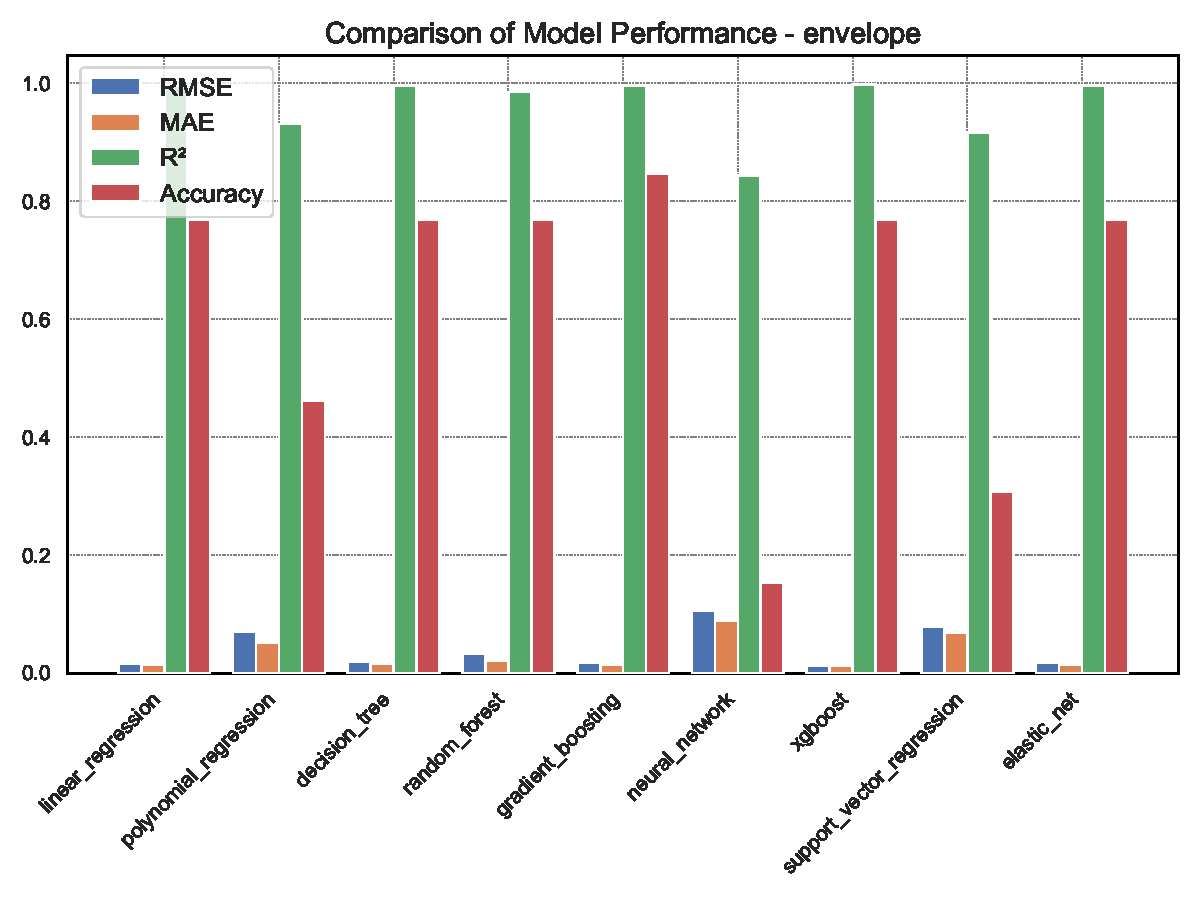
\includegraphics[width=\textwidth]{assets/images/05/performance_by_model_envelope}
        \caption{Envelope}
    \end{subfigure}
    \hfill
    \begin{subfigure}[t]{0.32\textwidth}
        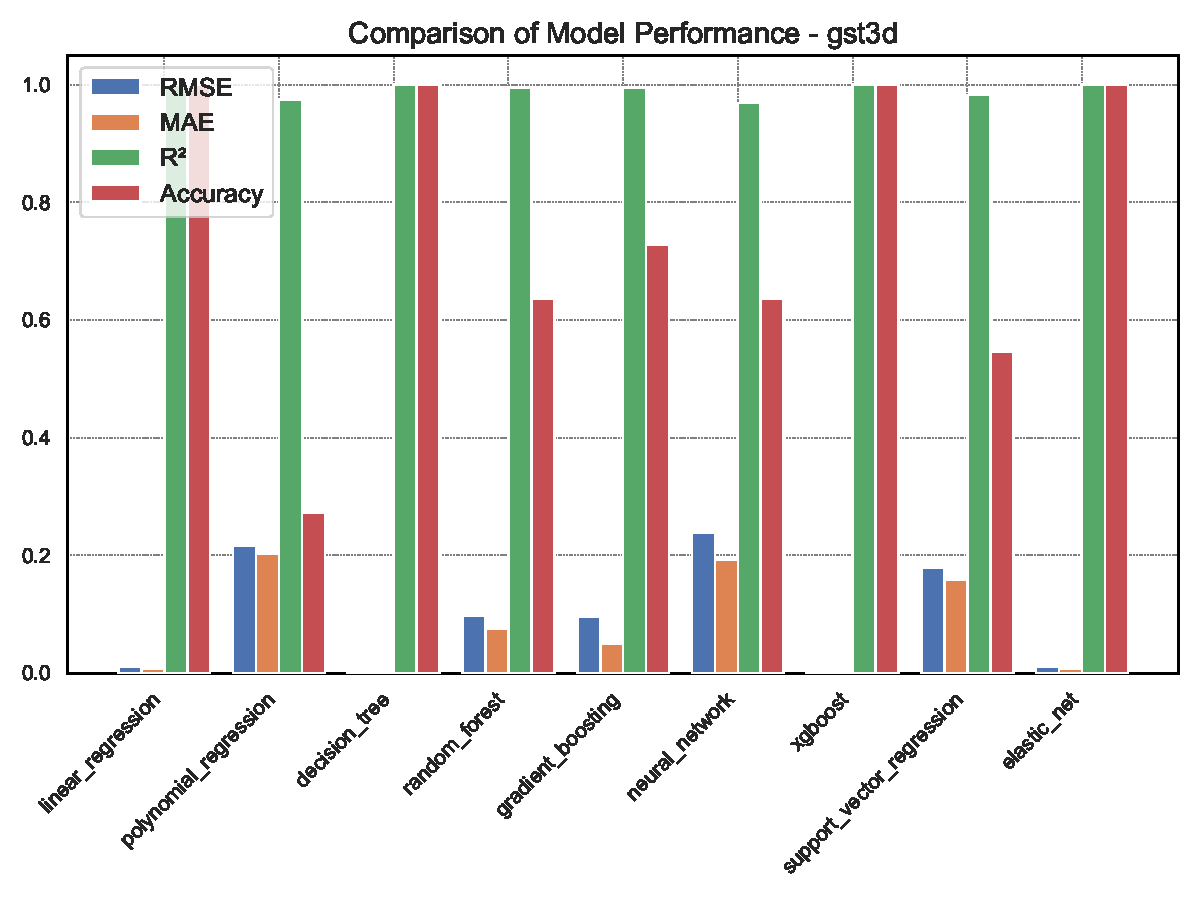
\includegraphics[width=\textwidth]{assets/images/05/performance_by_model_gst3d}
        \caption{\ac{GST3D}}
    \end{subfigure}
    \hfill
    \begin{subfigure}[t]{0.32\textwidth}
        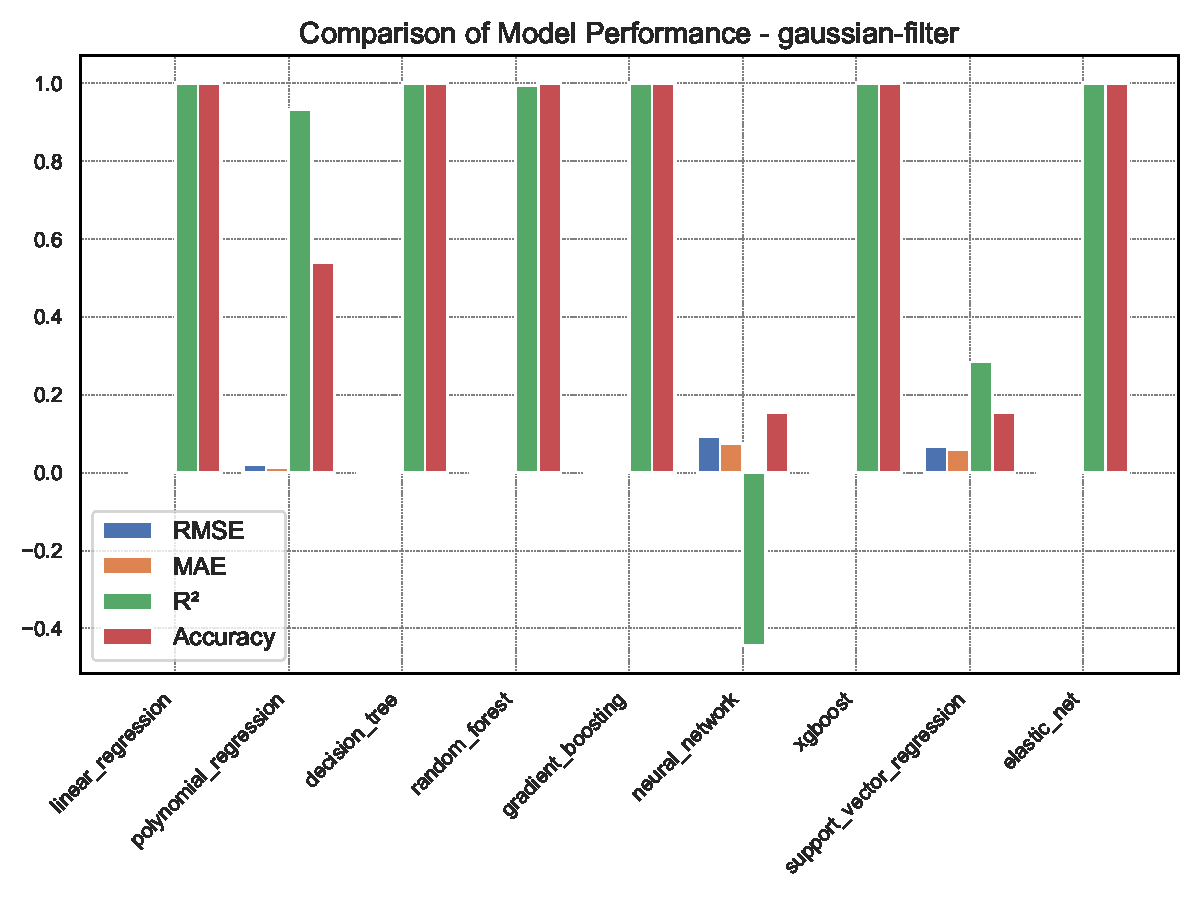
\includegraphics[width=\textwidth]{assets/images/05/performance_by_model_gaussian-filter}
        \caption{Gaussian Filter}
    \end{subfigure}
    \caption{Model metrics (\ac{RMSE}, \ac{MAE}, $R^2$, and accuracy) by operator.
        Best-in-class methods include Gradient Boosting (Envelope), Decision Tree (\ac{GST3D}), and Linear Regression (Gaussian Filter).
        \EB{Daniel, uma avaliação com valores RMSE e MAE deve levar em consideração o valor da predição - p.ex., um erro (RMSE ou MAE) de 0.1GB é pequeno em uma situação onde o valor real/predito é da ordem de dezenas ou centenas de GBs, no entanto, se o valor real/predito é da ordem de 0.1GB, o erro é bem grande.}
        \label{fig:performance_by_model_operators}
    }
\end{figure*}

In summary, the near-linear dependence of peak memory on shape parameters enables multiple models to achieve excellent accuracy and reliability.
Envelope and Gaussian Filter place fewer demands on model complexity.
\ac{GST3D} remains more challenging, though tree-based models and linear approaches still achieve high $R^2$ and low error metrics.
Neural Network stands out for relatively weaker performance in \ac{GST3D}, suggesting that the chosen architecture or hyperparameters might require further tuning for more complex operators.

All subsequent sections build on these findings to evaluate feature selection (Section~\ref{sec:pmc-results-feature-selection-experiments}) and data size reductions (Section~\ref{sec:pmc-results-data-reduction-studies}), aiming to determine whether simpler input representations or smaller datasets can maintain the strong predictive performance observed in these experiments.
\section{Feature Selection Experiments}
\label{sec:pmc-results-feature-selection-experiments}

\EB{Daniel, me parece que seria mais natural apresentar o processo de seleção de features antes das seções que realizam a análise dos dados já pressupondo o uso da feature volume.}

This section investigates the impact of eliminating various shape-derived features on model accuracy, with a particular focus on verifying whether \emph{volume} alone is \EBC{sufficient to predict peak memory usage}{Você já mostrou que a feature volume tem uma relação bem simples (linear) com o pico de consumo de memória.}.
Section~\ref{sec:pmc-results-model-performance-overview} identified Gradient Boosting, Linear Regression, and Decision Tree as the best performers for Envelope, Gaussian Filter, and \ac{GST3D}, respectively.
Consequently, the experiments below use these three models when removing features.

\subsection{Volume-Centric Hypothesis}
\label{subsec:feature-selection-volume-centric-hypothesis}

Figure~\ref{fig:memory_vs_volume_regression_subplots} shows how tightly memory usage correlates with volume for Envelope, Gaussian Filter, and \ac{GST3D}.
Each subplot includes a regression fit, highlighting that volume on its own explains most of the variance.
This observation motivates a systematic “feature pruning” study to confirm whether additional descriptors (e.g., diagonal length, surface area, ratio features) offer meaningful improvements.

\begin{figure*}[htbp]
    \centering
    \begin{subfigure}[t]{0.32\textwidth}
        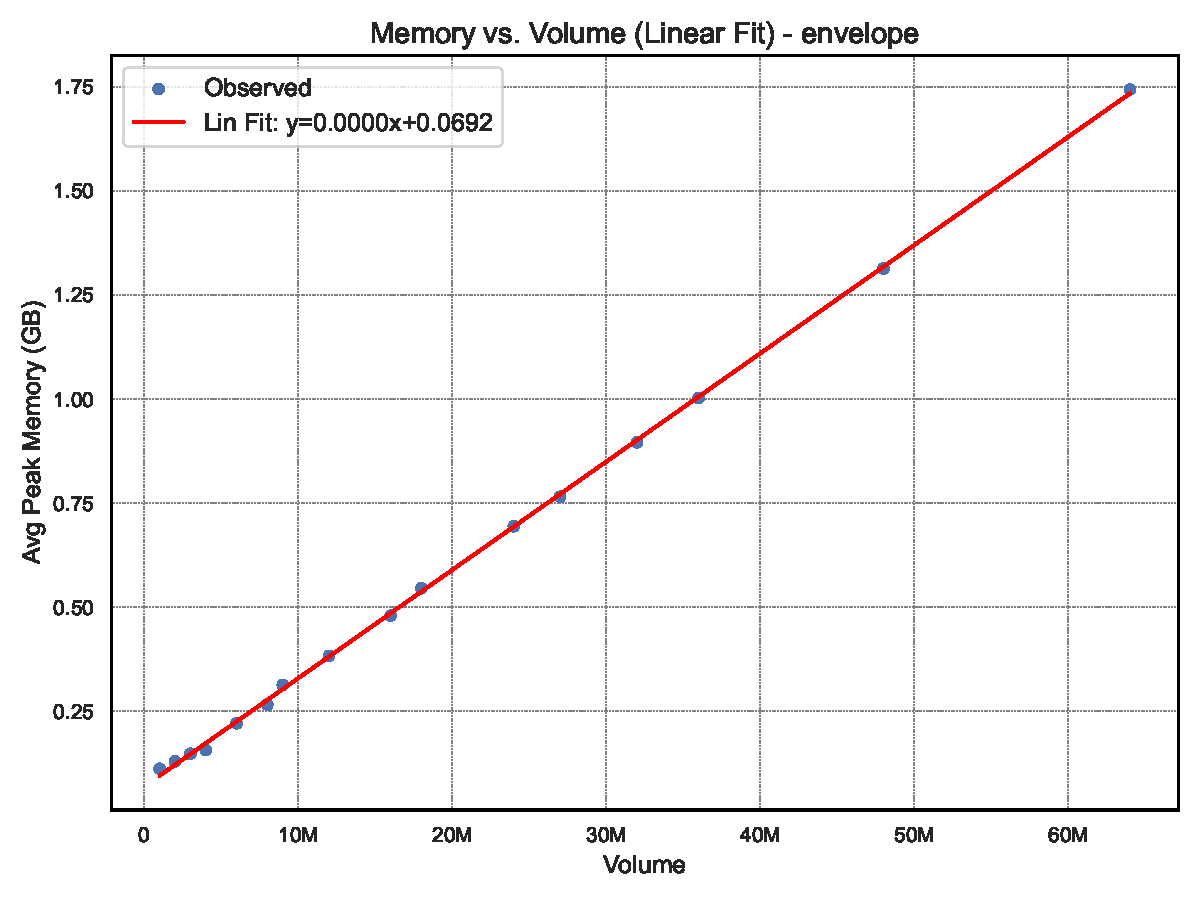
\includegraphics[width=\textwidth]{assets/images/05/memory_vs_volume_regression_envelope}
        \caption{Envelope}
    \end{subfigure}
    \hfill
    \begin{subfigure}[t]{0.32\textwidth}
        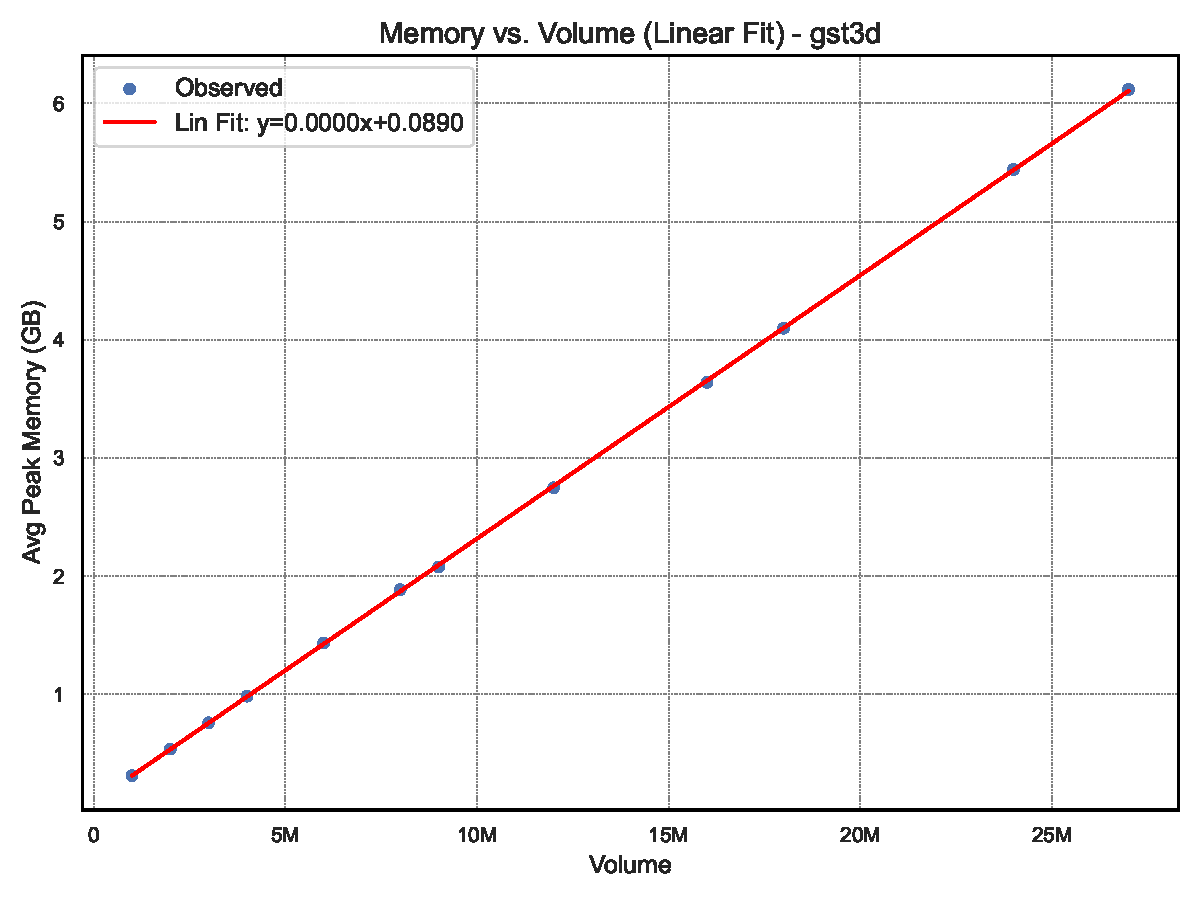
\includegraphics[width=\textwidth]{assets/images/05/memory_vs_volume_regression_gst3d}
        \caption{\ac{GST3D}}
    \end{subfigure}
    \hfill
    \begin{subfigure}[t]{0.32\textwidth}
        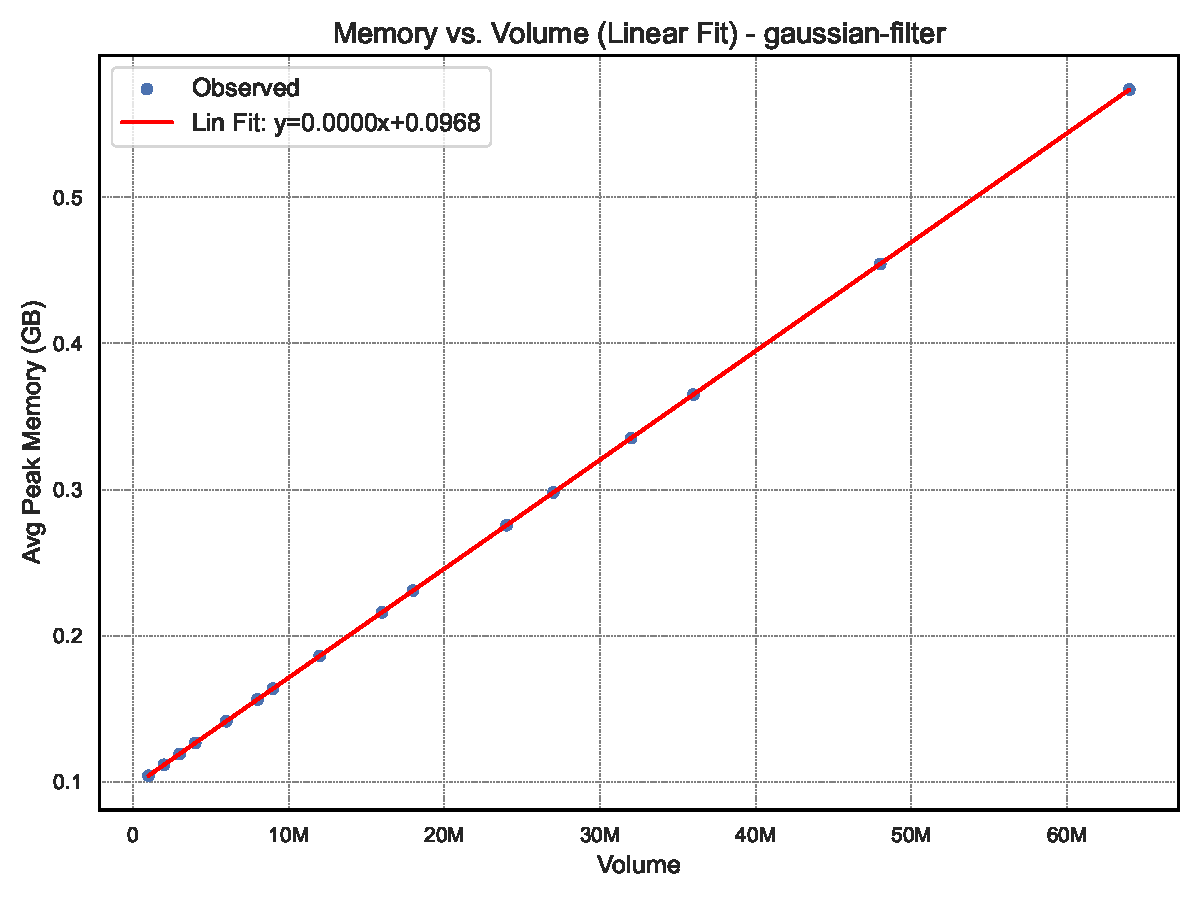
\includegraphics[width=\textwidth]{assets/images/05/memory_vs_volume_regression_gaussian-filter}
        \caption{Gaussian Filter}
    \end{subfigure}
    \caption{Memory usage vs.\ volume with regression lines for Envelope, \ac{GST3D}, and Gaussian Filter.
    All three curves reinforce that volume alone has substantial explanatory power.}
    \label{fig:memory_vs_volume_regression_subplots}
\end{figure*}

\subsection{Feature Removal Process and Metrics}
\label{subsec:feature-removal-methods-and-metrics}

The experiments adopted a stepwise strategy:
\begin{enumerate}
    \item Collect a ranked list of features using a relevance metric (e.g., \emph{SelectKBest}). \EB{Senti falta de uma explicação e/ou referências para o método SelectKBest e uma breve discussão sobre como você aplicou ele - aplicou múltiplas vezes, uma para cada modelo? Uma para cada operador? uma única vez e gerou um único ranking? Esta parte dos resultados está bem obscura.}
    \item Remove the least-relevant feature and retrain the model.
    \item Document changes in \ac{RMSE}, \ac{MAE}, $R^2$, accuracy, and a combined “score.”
    \item Repeat until only \emph{volume} remains.
\end{enumerate}
Table~\ref{tab:feature_selection_minimal_impact} highlights selected examples of Envelope and Gaussian Filter runs, showing how the \ac{RMSE} and $R^2$ shift little upon discarding most auxiliary features.
In nearly all cases, \emph{volume} was never dropped, confirming its primacy in determining memory usage.
\EB{O que acontece se você remover apenas a feature volume?}

\begin{table}[htbp]
    \centering
    \begin{tabular}{lcccccc}
        \hline
        \textbf{Operator} & \textbf{Num.\ Features} & \textbf{Model}    & \textbf{\ac{RMSE}}       & \textbf{$R^2$} & \textbf{Score} & \textbf{Comment} \\
        \hline
        Envelope          & 25                      & Gradient Boosting & 0.0167                   & 0.9961         & 2.5794         & Full set          \\
        Envelope          & 3                       & Gradient Boosting & 0.0150                   & 0.9969         & 2.5823         & Volume + 2 others \\
        \hline
        \ac{GST3D}        & 25                      & Decision Tree     & 0.0023363                & 0.9999970      & 2.9697         & Full set          \\
        \ac{GST3D}        & 3                       & Decision Tree     & 0.0038614                & 0.9999918      & 2.9673         & Volume + 2 others \\
        \hline
        Gaussian Filter   & 25                      & Linear Regression & \(\,2.4 \times 10^{-5}\) & 0.9999999      & 2.9045         & Full set          \\
        Gaussian Filter   & 3                       & Linear Regression & \(\,2.2 \times 10^{-5}\) & 0.9999999      & 2.9045         & Volume + 2 others \\
        \hline
    \end{tabular}
    \caption{Subset of feature-removal results for Envelope, \ac{GST3D}, and Gaussian Filter.
        \ac{RMSE} and $R^2$ remain largely stable as the number of predictors decreases, implying that volume has the dominant role.
        \EB{Corrigir invasão de margem.}
        \label{tab:feature_selection_minimal_impact}
    }
\end{table}

\subsection{Impact on RMSE, R\texorpdfstring{$^2$}{2}, and Residuals}
\label{subsec:impact-on-rmse-r2-and-residuals}

Figures~\ref{fig:feature_selection_overview_part1}--\ref{fig:feature_selection_overview_part2} illustrate the marginal effect of dropping features across operators.
Panel~(a) in Figure~\ref{fig:feature_selection_overview_part1} shows how the \ac{RMSE} changes slightly or not at all when each feature is removed, averaged over multiple runs.
Panel~(b) displays the same logic for $R^2$ scores.
Both metrics exhibit negligible variations except when volume is excluded, which severely degrades performance.

\begin{figure*}[htbp]
    \centering
    \begin{subfigure}[t]{0.49\textwidth}
        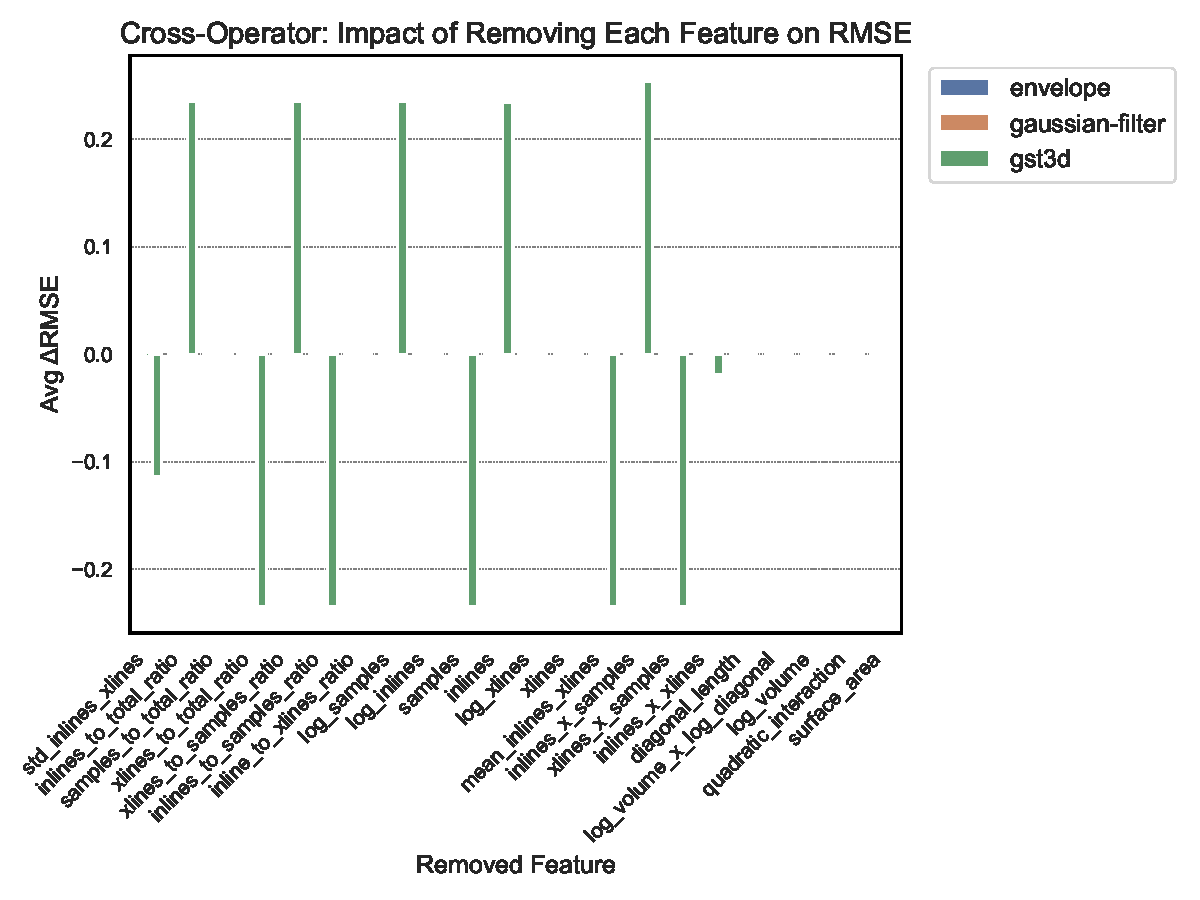
\includegraphics[width=\textwidth]{assets/images/05/feature_impact}
        \caption{Average \ac{RMSE} change per feature removal.
        Smaller bars indicate minimal impact.}
    \end{subfigure}
    \hfill
    \begin{subfigure}[t]{0.49\textwidth}
        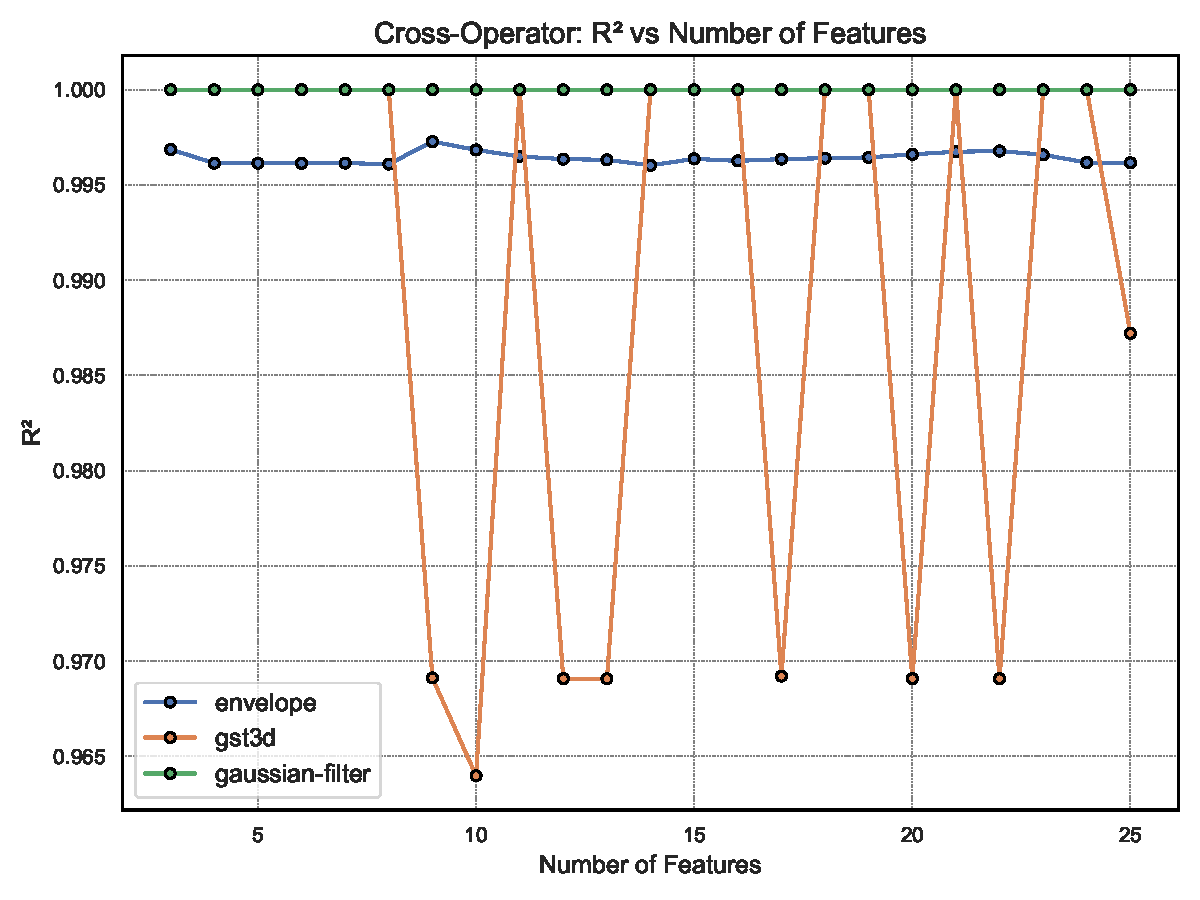
\includegraphics[width=\textwidth]{assets/images/05/cross_feature_selection_r2}
        \caption{$R^2$ changes during progressive feature removal across all operators.
        Volume stands out as indispensable.}
    \end{subfigure}
    \caption{Feature-removal impacts.
        Volume consistently emerges as the most critical input, whereas removing others typically yields negligible performance changes.
        \EB{Para argumentar que o volume é feature mais importante, não seria necessário mostrar que a remoção dela reduz o desempenho dos modelos?}
        \label{fig:feature_selection_overview_part1}
    }
\end{figure*}

Figure~\ref{fig:feature_selection_overview_part2} extends the analysis to residual-distribution metrics.
In particular, part~(b) shows that any small spikes in the residual curves do not substantially alter the final predictive reliability.
Hence, even simplified models (volume plus one or two shape parameters) are nearly as accurate as the full 25-feature configurations.

\begin{figure*}[htbp]
    \centering
    \begin{subfigure}[t]{0.49\textwidth}
        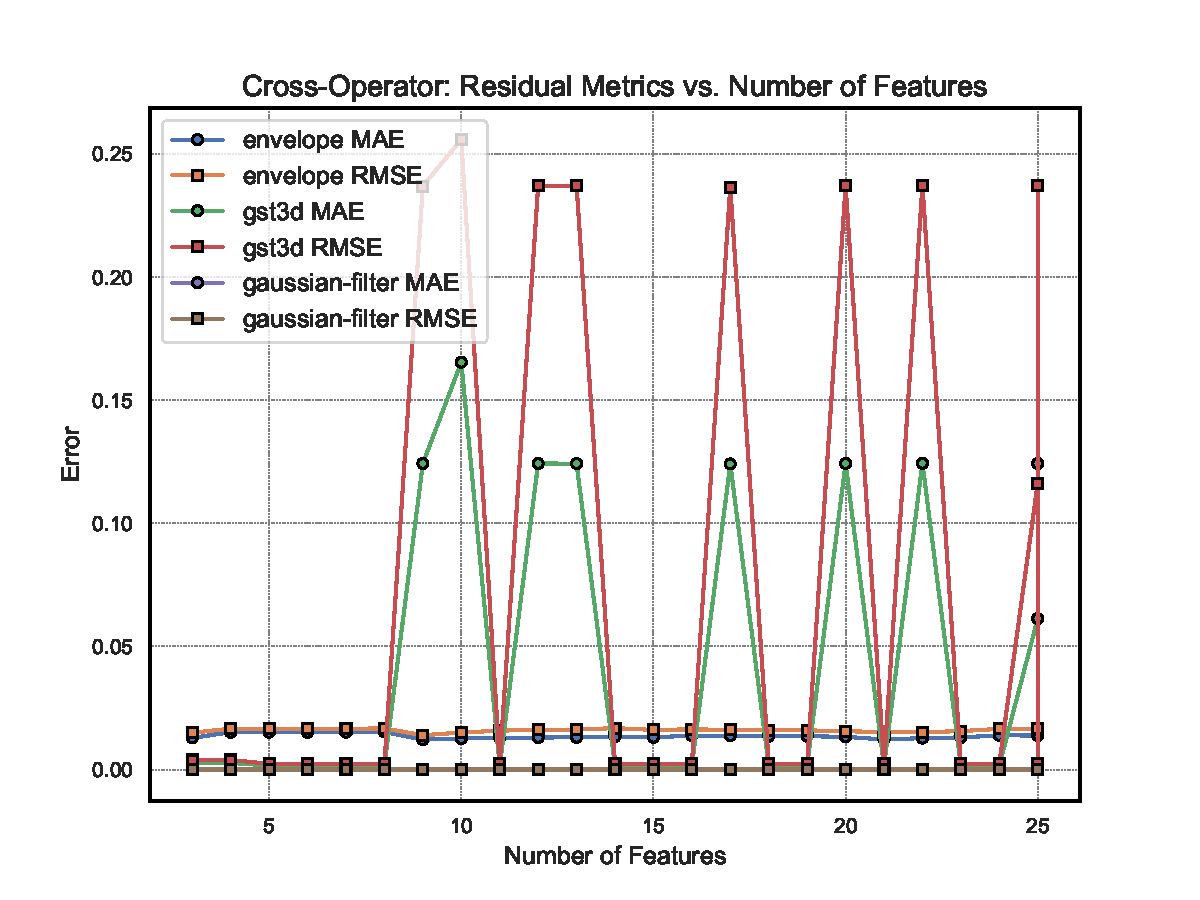
\includegraphics[width=\textwidth]{assets/images/05/residual_metrics_by_number_of_features}
        \caption{Residual-based metrics vs.\ number of features.
        Most fluctuations are minor.}
    \end{subfigure}
    \hfill
    \begin{subfigure}[t]{0.49\textwidth}
        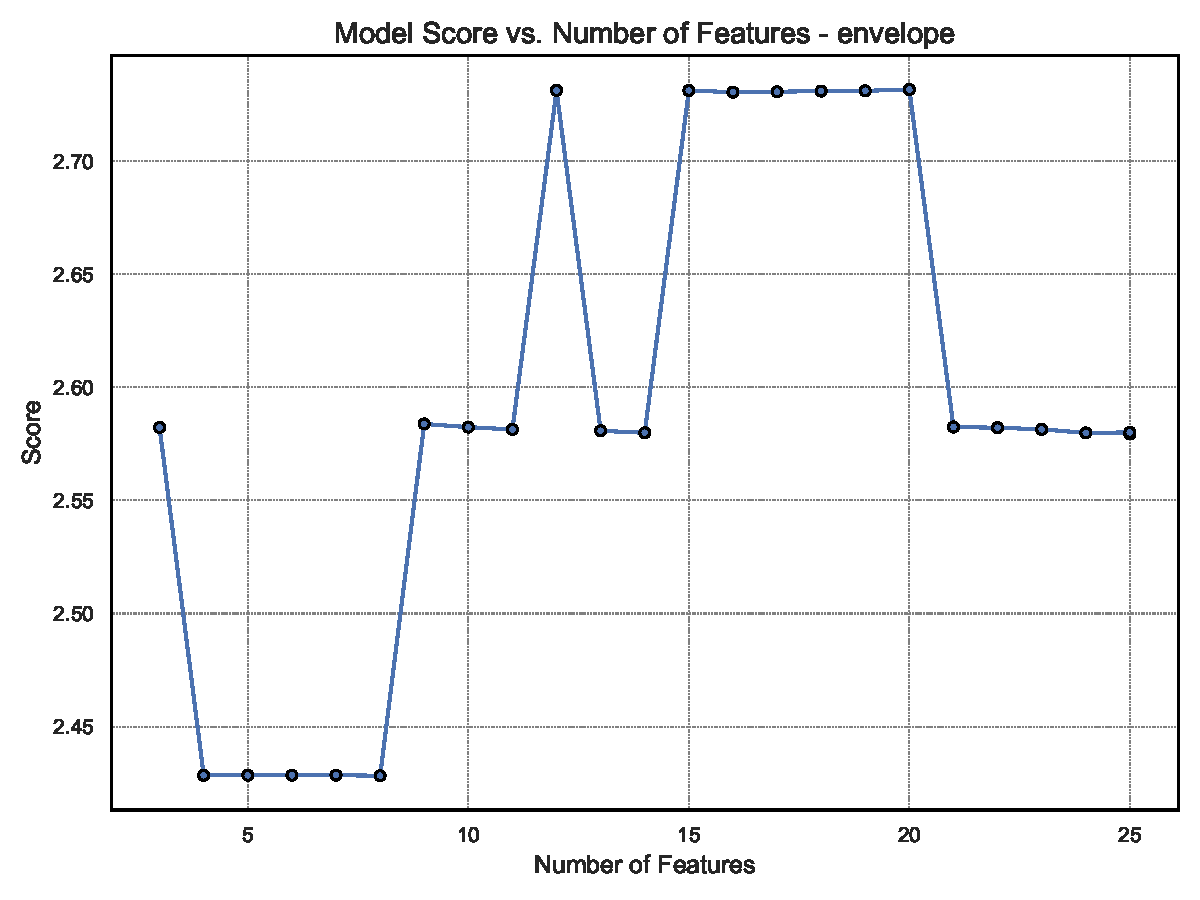
\includegraphics[width=\textwidth]{assets/images/05/score_by_number_of_features_envelope}
        \caption{Envelope example: overall “score” across successive feature removals.
        Scores remain stable or slightly improve.}
    \end{subfigure}
    \caption{Residual and score patterns under feature removal.
    Even with fewer predictors, model performance remains robust.}
    \label{fig:feature_selection_overview_part2}
\end{figure*}

\subsection{Operator-Specific Breakdown}
\label{subsec:operator-specific-breakdown}

Figures~\ref{fig:feature_impact_operator_subplots} and~\ref{fig:residual_metrics_by_number_of_features_operator_subplots} provide per-operator plots of the incremental feature-importance measurements.
The Envelope plots confirm that volume alone can achieve a \ac{RMSE} as low as 0.015.
Gaussian Filter achieves a \ac{RMSE} near \(2\times10^{-5}\) with only volume.
\ac{GST3D} benefits marginally from including another parameter (e.g., diagonal length), but dropping everything except \EBADD{the} volume \EBADD{efature} still yields strong $R^2 \approx 0.9999$ in many runs.

\begin{figure*}[htbp]
    \centering
    \begin{subfigure}[t]{0.32\textwidth}
        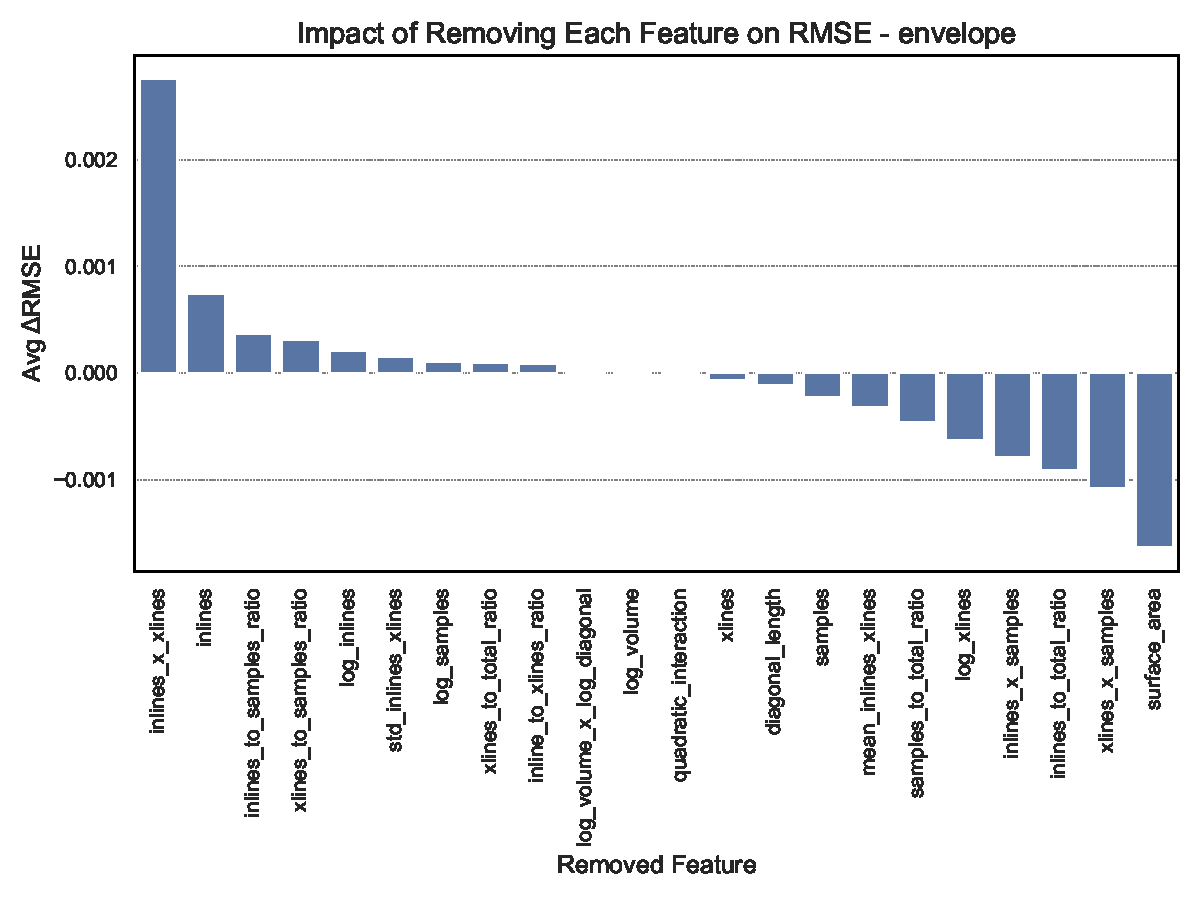
\includegraphics[width=\textwidth]{assets/images/05/feature_impact_envelope}
        \caption{Envelope}
    \end{subfigure}
    \hfill
    \begin{subfigure}[t]{0.32\textwidth}
        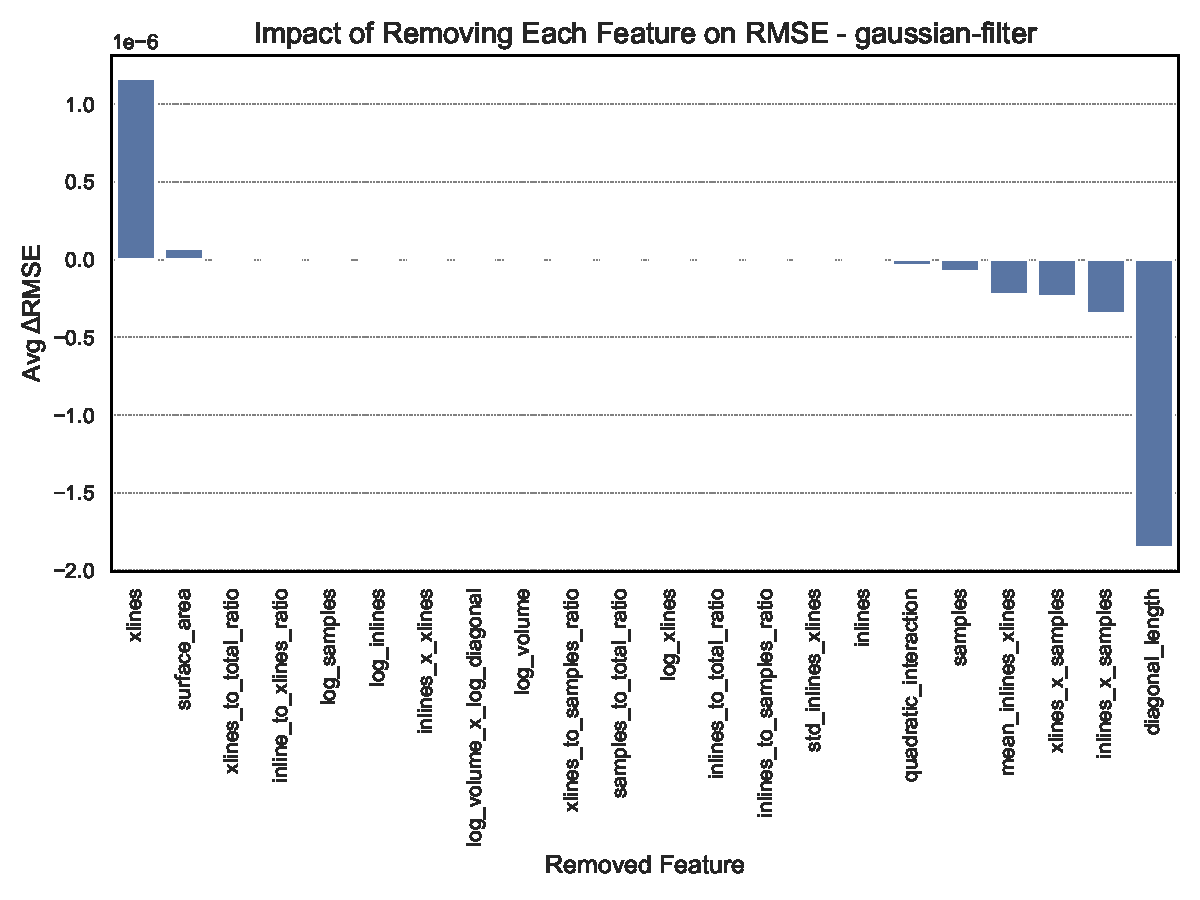
\includegraphics[width=\textwidth]{assets/images/05/feature_impact_gaussian-filter}
        \caption{Gaussian Filter}
    \end{subfigure}
    \hfill
    \begin{subfigure}[t]{0.32\textwidth}
        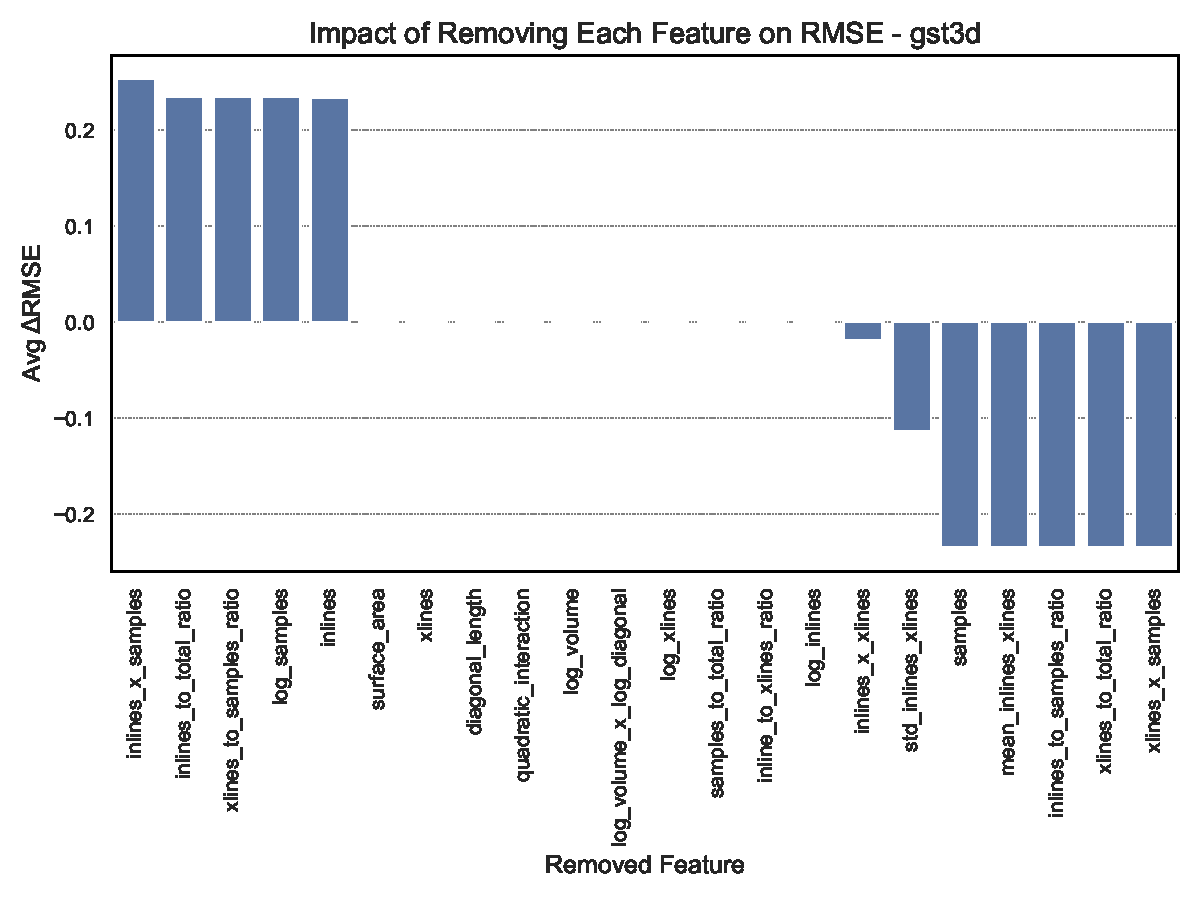
\includegraphics[width=\textwidth]{assets/images/05/feature_impact_gst3d}
        \caption{\ac{GST3D}}
    \end{subfigure}
    \caption{Feature-removal impact by operator.
        Bars represent the increase in \ac{RMSE} (or other metrics) upon discarding each feature.
        Volume is consistently the most essential.
        \EB{Que tal usar "Number of features removed" em vez de "Number of features" no eixo-x dos gráficos?}
        \EB{BTW, talvez fique melhor usar o mesmo eixo-y (mesmo intervalo no eixo-y) nos três gráficos.}
        \label{fig:feature_impact_operator_subplots}
    }
\end{figure*}

\begin{figure*}[htbp]
    \centering
    \begin{subfigure}[t]{0.32\textwidth}
        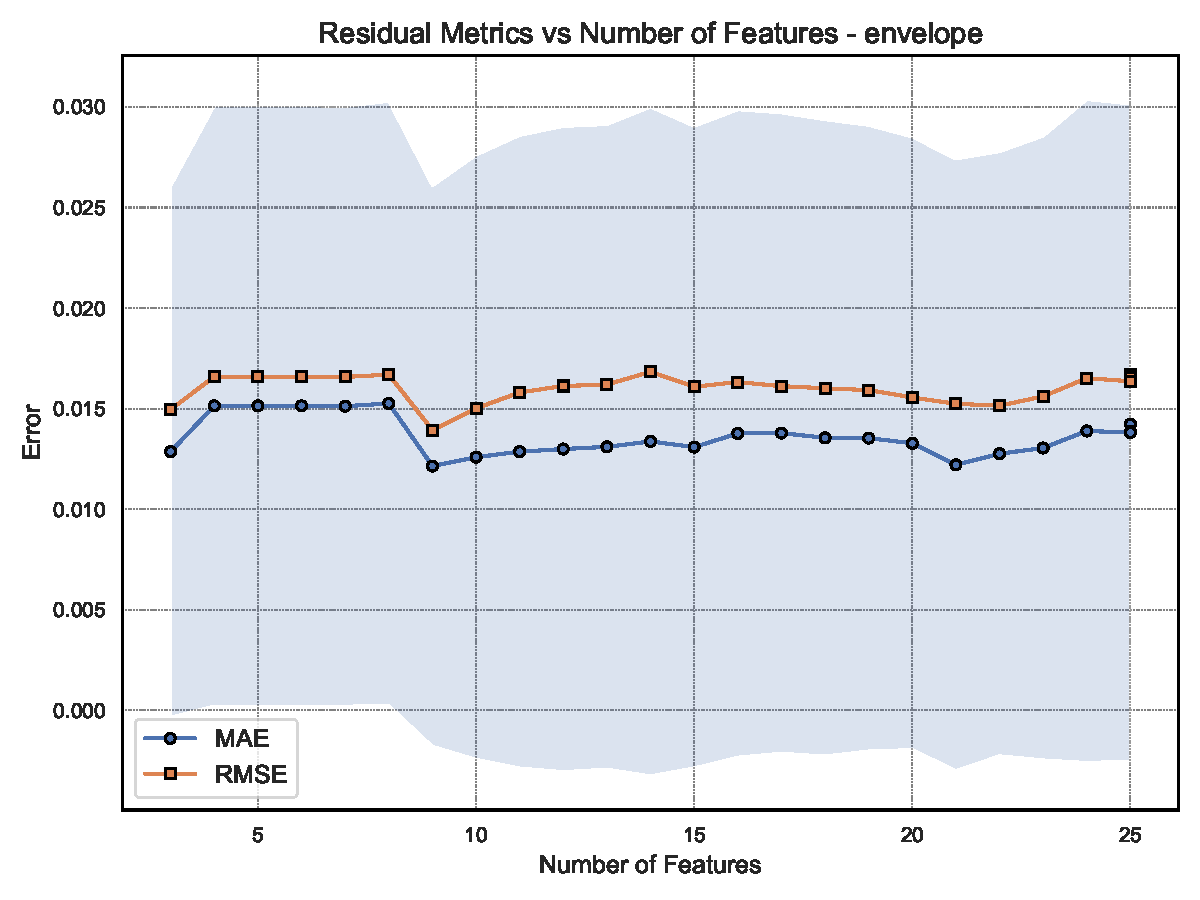
\includegraphics[width=\textwidth]{assets/images/05/residual_metrics_by_number_of_features_envelope}
        \caption{Envelope}
    \end{subfigure}
    \hfill
    \begin{subfigure}[t]{0.32\textwidth}
        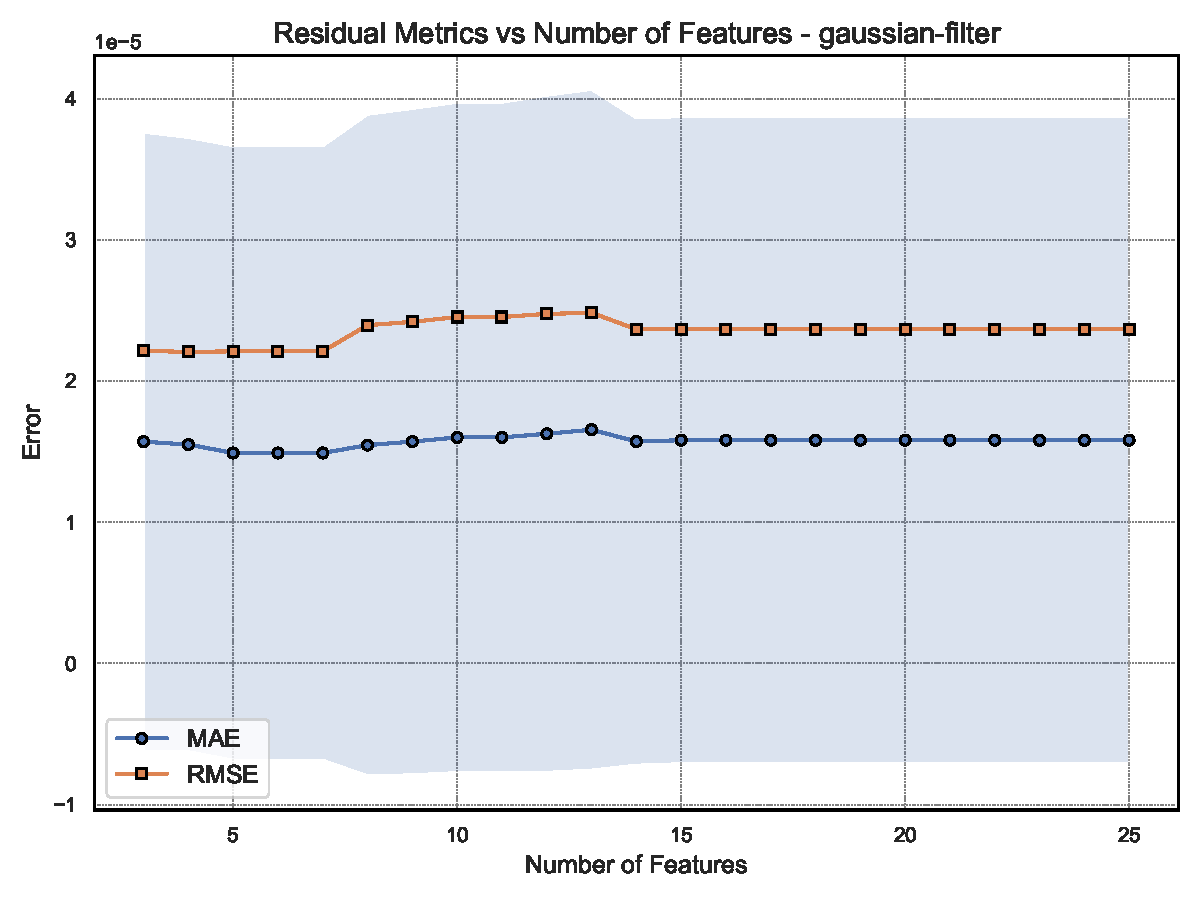
\includegraphics[width=\textwidth]{assets/images/05/residual_metrics_by_number_of_features_gaussian-filter}
        \caption{Gaussian Filter}
    \end{subfigure}
    \hfill
    \begin{subfigure}[t]{0.32\textwidth}
        \includegraphics[width=\textwidth]{assets/images/05/residual_metrics_by_number_of_features_gst3d}
        \caption{\ac{GST3D}}
    \end{subfigure}
    \caption{Residual metrics versus number of features, split by operator.
    Envelope and Gaussian Filter are especially insensitive to feature reductions.
    \ac{GST3D} shows slightly larger performance dips when discarding non-volume inputs.}
    \label{fig:residual_metrics_by_number_of_features_operator_subplots}
\end{figure*}

\subsection{Summary of Findings}
\label{subsec:feature-selection-summary}

Collectively, these results support the conclusion that volume alone explains most memory usage variance in the tested seismic operators.
Limited improvements arise from including additional geometric attributes, yet the gain is usually minor.
Volume consistently appears in the top rank when applying \emph{SelectKBest} or other scoring schemes.
This aligns with earlier evidence of near-linear volume scaling (Section~\ref{sec:pmc-results-memory-and-execution-time-profiling}).

Practitioners seeking a lightweight memory-usage estimator can therefore rely on volume as the central input feature.
The next section investigate further data reduction (Section~\ref{sec:pmc-results-data-reduction-studies}) to refine the broader performance picture.
% like we did on feature selection, we tried to remove the amount of samples while testing the models. What we did was basically remove the "mean". So, we looked at the volume, kept the extremas, and removed (uniformly) the "middle"
% charts assets/images/05/cross_data_reduction_rmse.pdf and residual_metrics_by_sample_size.pdf show that the performance decreases. We can see that the RMSE increases, and the other metrics also increase. This is expected, since we are removing samples
% chart assets/images/05/metrics_evolution_by_sample_size.pdf show this as an overview by comparing all metrics in a facet for all operators
% charts assets/images/05/residual_metrics_by_sample_size_envelope.pdf, assets/images/05/residual_metrics_by_sample_size_gaussian-filter.pdf, and assets/images/05/residual_metrics_by_sample_size_gst3d.pdf show that the error metrics increase both in variability, as well as size, when we reduce the number of samples. We can see that it kepts some sort of stable until ~30 samples, and then it starts to increase
% charts assets/images/05/metrics_evolution_by_sample_size_envelope.pdf, assets/images/05/metrics_evolution_by_sample_size_gaussian-filter.pdf, and assets/images/05/metrics_evolution_by_sample_size_gst3d.pdf show all the metrics in a facet for each operator, showing that the error metrics increase when we reduce the number of samples
% charts assets/images/05/score_by_sample_size_envelope.pdf, assets/images/05/score_by_sample_size_gaussian-filter.pdf, and assets/images/05/score_by_sample_size_gst3d.pdf show the score of the models when we reduce the number of samples. We can see that the score decreases as we reduce the number of samples. But we also see that until ~30 it decreases slightly
% as we can see, we have a sweet spot close to 30

\section{Data Reduction Studies}
\label{sec:pmc-results-data-reduction-studies}

\EB{Acho que seria bom usar um título mais específico. Algo como: "Training Set Size", "Training Set Reduction Studies", "Impact of training set size"...}

This section discusses how predictive accuracy changes when the training dataset is subsampled, thus reducing the total number of configurations.
The aim is to identify whether smaller subsets of shape–memory measurements can still produce reliable models.
Specifically, experiments removed “middle-range” samples of the volume dimension (or shape parameters more broadly), keeping the smallest and largest volumes, while uniformly discarding intermediate sizes.
Both Envelope and \ac{GST3D} used the best models identified (Gradient Boosting and Decision Tree, respectively), while Gaussian Filter used Linear Regression.

\EB{Esta seção é bem interessante e importante. No entanto, a decisão de usar volumes pequenos e grandes em vez de pequenos e médios me pareceu arbitrária. Em tese, seria melhor usar pequenos e médios, já que o custo de coletar estes dados é menor.}

\subsection{Subsampling Strategy and Motivation}
\label{subsec:data-reduction-strategy-and-motivation}

The data-reduction procedure systematically excludes shape configurations from the central volume interval, retaining the extremes that often yield the highest or lowest memory usage.
By gradually lowering the sample count (\(N\)), it is possible to observe how model performance deteriorates or remains stable.
Figures~\ref{fig:cross_data_reduction_and_residual}--\ref{fig:metrics_evolution_sample_size_operators} present the overall results.
Figure~\ref{fig:cross_data_reduction_and_residual}(a) plots the \ac{RMSE} as a function of sample size, while part~(b) shows how residual-based metrics evolve.
All three operators suffer performance degradation under severe reductions, but moderate cutbacks can still yield acceptable accuracy.

\begin{figure*}[htbp]
    \centering
    \begin{subfigure}[t]{0.49\textwidth}
        \includegraphics[width=\textwidth]{assets/images/05/cross_data_reduction_rmse}
        \caption{\ac{RMSE} across Envelope, \ac{GST3D}, and Gaussian Filter as sample size decreases.
            A smooth upward trend reflects the increasing difficulty of fitting with fewer examples.
            \EB{Por que escolheu o RMSE em vez do outro score?}
        }
    \end{subfigure}
    \hfill
    \begin{subfigure}[t]{0.49\textwidth}
        \includegraphics[width=\textwidth]{assets/images/05/residual_metrics_by_sample_size}
        \caption{Residual metrics also climb with smaller datasets.
        Minimal sets (\(<20\) samples) show large spikes, indicating insufficient coverage of intermediate volumes.}
    \end{subfigure}
    \caption{Data-reduction effects, viewed globally for all operators.
        Reducing the training set drives up errors and variability.
        \EB{Estes dois gráficos são bem parecidos. Faz sentido manter os dois. Talvez o da esquerda já seja suficiente.}
        \label{fig:cross_data_reduction_and_residual}
    }
\end{figure*}

\subsection{Operator-Wise Performance Trends}
\label{subsec:operator-wise-sample-size-analysis}

Figures~\ref{fig:residual_metrics_by_sample_size_operators}--\ref{fig:metrics_evolution_sample_size_operators} elaborate on each operator individually.
When sample sizes fall below roughly 30, \ac{RMSE}, \ac{MAE}, and residual variance begin to rise more sharply.
This pattern is consistent with the notion that “filling in” the middle range of volumes is essential for maintaining a robust regression fit.
However, moderately pruned datasets (e.g., 40–50 samples) still achieve respectable $R^2 > 0.98$ in most cases, as verified by the CSV results in Table~\ref{tab:data_reduction_summary}. \EB{Referência quebrada}

\begin{figure*}[htbp]
    \centering
    \begin{subfigure}[t]{0.32\textwidth}
        \includegraphics[width=\textwidth]{assets/images/05/residual_metrics_by_sample_size_envelope}
        \caption{Envelope}
    \end{subfigure}
    \hfill
    \begin{subfigure}[t]{0.32\textwidth}
        \includegraphics[width=\textwidth]{assets/images/05/residual_metrics_by_sample_size_gaussian-filter}
        \caption{Gaussian Filter}
    \end{subfigure}
    \hfill
    \begin{subfigure}[t]{0.32\textwidth}
        \includegraphics[width=\textwidth]{assets/images/05/residual_metrics_by_sample_size_gst3d}
        \caption{\ac{GST3D}}
    \end{subfigure}
    \caption{Residual-based metrics per operator as sample size diminishes.
    Error bars reflect increasing variability at smaller dataset sizes.}
    \label{fig:residual_metrics_by_sample_size_operators}
\end{figure*}

\begin{figure*}[htbp]
    \centering
    \begin{subfigure}[t]{0.32\textwidth}
        \includegraphics[width=\textwidth]{assets/images/05/metrics_evolution_by_sample_size_envelope}
        \caption{Envelope}
    \end{subfigure}
    \hfill
    \begin{subfigure}[t]{0.32\textwidth}
        \includegraphics[width=\textwidth]{assets/images/05/metrics_evolution_by_sample_size_gaussian-filter}
        \caption{Gaussian Filter}
    \end{subfigure}
    \hfill
    \begin{subfigure}[t]{0.32\textwidth}
        \includegraphics[width=\textwidth]{assets/images/05/metrics_evolution_by_sample_size_gst3d}
        \caption{\ac{GST3D}}
    \end{subfigure}
    \caption{All metrics tracked as sample sizes drop, plotted per operator.
        \ac{RMSE} and \ac{MAE} grow steadily, while $R^2$ and accuracy decline.}
    \label{fig:metrics_evolution_sample_size_operators}
\end{figure*}

\subsection{Score Comparisons and Sweet Spot Around 30 Samples}
\label{subsec:score-comparisons-and-sweet-spot}

Figures~\ref{fig:score_by_sample_size_operators}(a)–(c) plot the consolidated “score” metric described in Section~\ref{sec:pmc-results-model-performance-overview}.
All three operators see an inflection around 30–35 samples where model quality remains strong.
Below that threshold, the curves dip more significantly, reflecting the loss of mid-range volume coverage.
Above 40–50 samples, the gains saturate, and further additions of similar configurations do not yield major improvements.

\begin{figure*}[htbp]
    \centering
    \begin{subfigure}[t]{0.32\textwidth}
        \includegraphics[width=\textwidth]{assets/images/05/score_by_sample_size_envelope}
        \caption{Envelope}
    \end{subfigure}
    \hfill
    \begin{subfigure}[t]{0.32\textwidth}
        \includegraphics[width=\textwidth]{assets/images/05/score_by_sample_size_gaussian-filter}
        \caption{Gaussian Filter}
    \end{subfigure}
    \hfill
    \begin{subfigure}[t]{0.32\textwidth}
        \includegraphics[width=\textwidth]{assets/images/05/score_by_sample_size_gst3d}
        \caption{\ac{GST3D}}
    \end{subfigure}
    \caption{Model scores vs.\ sample size.
    Each operator shows a notable decline below \(\sim\)30 samples, marking a practical lower bound for training.}
    \label{fig:score_by_sample_size_operators}
\end{figure*}

Table~\ref{tab:data_reduction_summary} illustrates partial data from the CSV logs (see \texttt{envelope.csv}, \texttt{gaussian-filter.csv}, and \texttt{gst3d.csv}). 
\EB{Corrigir a Referência quebrada e a invasão de margem.}
It includes selected sample sizes and the resulting \ac{RMSE}, $R^2$, accuracy, and overall score.
Even moderate subsampling (34 or 42 samples, for instance) still achieves high $R^2$ for Envelope and Gaussian Filter.
\ac{GST3D} remains more sensitive, though a subset of 44 samples can deliver near-perfect accuracy.

\begin{table}[htbp]
    \centering
    \begin{tabular}{lccccc}
        \hline
        \textbf{Operator} & \textbf{\#Samples} & \textbf{\ac{RMSE}}    & \textbf{$R^2$} & \textbf{Accuracy} & \textbf{Score} \\
        \hline
        \multirow{3}{*}{\textbf{Envelope}}
        & 64                 & 0.0170                & 0.9959         & 0.8462            & 2.5789         \\
        & 34                 & 0.0217                & 0.9926         & 0.7143            & 2.3113         \\
        & 11                 & 0.2463                & 0.8805         & 0.3333            & 1.2155         \\
        \hline
        \multirow{3}{*}{\textbf{Gaussian Filter}}
        & 64                 & \(2.37\times10^{-5}\) & 0.9999999      & 1.0               & 2.9045         \\
        & 34                 & \(2.90\times10^{-5}\) & 0.9999998      & 1.0               & 2.9044         \\
        & 11                 & \(1.02\times10^{-4}\) & 0.9999997      & 1.0               & 2.9044         \\
        \hline
        \multirow{3}{*}{\textbf{\ac{GST3D}}}
        & 54                 & 0.2371                & 0.9691         & 0.7273            & 2.0478         \\
        & 29                 & 0.3689                & 0.9251         & 0.8333            & 2.0472         \\
        & 11                 & 1.1042                & 0.7684         & 0.0000            & -1.0768        \\
        \hline
    \end{tabular}
    \caption{Selected data-reduction results (largest, close to 30, smallest) for each operator.
    Subsets of around 30--40 samples retain robust accuracy, while very small sets
        (e.g., 11) cause steep performance declines, especially for \ac{GST3D}.}
    \label{tab:data_reduction_small_vs_medium_vs_large}
\end{table}

\subsection{Conclusions on Data Pruning}
\label{subsec:data-reduction-conclusions}

These experiments confirm that seismic-memory models require at least 30 samples to maintain stable performance, primarily to capture mid-scale volumes.
Envelope and Gaussian Filter remain accurate even with moderate data pruning, while \ac{GST3D} is somewhat more sensitive due to its heavier internal complexity.
Still, collecting 30–40 shape configurations seems sufficient for building robust predictive models without incurring excessive data-gathering overhead.
Subsequent sections integrate these findings with the feature-selection insights to propose minimal yet effective training strategies for real-world \ac{HPC} applications.